\documentclass[12pt]{report}

\usepackage[utf8]{inputenc}
\usepackage[T1]{fontenc}
\usepackage[a4paper,width=150mm,top=25mm,bottom=25mm]{geometry}
\usepackage{lmodern}
\usepackage{amsmath}
\usepackage{amsfonts}
\usepackage{amssymb}
\usepackage{relsize}
\usepackage{tikz}
\usepackage{tikz-cd}
\usepackage{mathtools}
\usepackage{wasysym}
\usepackage{float}
\usepackage{smartref}
\usepackage{amsthm}
\usepackage{setspace}
\usepackage{units}
\usepackage{textgreek}
\usepackage{hyperref}
\linespread{1.5}

\usepackage[linesnumbered,ruled,vlined]{algorithm2e}

\floatstyle{boxed}
\restylefloat{figure}

\usetikzlibrary{matrix}

\newcommand{\I}{\mathbb{I}}
\newcommand{\N}{\mathbb{N}}
\newcommand{\F}{\mathcal{F}}
\newcommand{\tF}{\thicktilde{\F}}
\newcommand{\Z}{\mathbb{Z}}
\newcommand{\RP}{\mathbb{RP}}
\newcommand{\R}{\mathbb{R}}
\newcommand{\RR}{\R^2}
\newcommand{\RRN}{\R^n}
\newcommand{\RNP}{\R_+^n}
\newcommand{\RNPP}{\R_{++}^n}
\newcommand{\C}{\mathbb{C}}
\newcommand{\CP}{\mathbb{CP}}
\newcommand{\D}{\mathbb{D}}
\newcommand{\DD}{\D^2}
\newcommand{\DN}{\D^n}
\newcommand{\HH}{\mathbb{H}}
\newcommand{\HN}{\mathbb{H}^n}
\newcommand{\dd}{\; \mathrm{d}}
\newcommand{\res}{\;\mathrm{res}}
\newcommand{\id}{\mathrm{id}}
\newcommand{\img}{\,\mathrm{im}\,}
\newcommand{\coker}{\,\mathrm{coker}\,}

\newcommand{\gm}{\mathfrak{m}}
\newcommand{\gp}{\mathfrak{p}}
\newcommand{\tensr}{\otimes_R}
\newcommand{\tens}{\otimes}


\newcommand{\ddz}{\;\mathrm{d}z}
\newcommand{\ddx}{\;\mathrm{d}x}
\newcommand{\ddy}{\;\mathrm{d}y}
\newcommand{\ddt}{\;\mathrm{d}t}
\newcommand{\pd}{\partial}
\newcommand{\pdx}{\partial_x}
\newcommand{\pdy}{\partial_y}

\newcommand{\dxdt}{\frac{dx}{dt}}
\newcommand{\dydt}{\frac{dy}{dt}}
\newcommand{\dydx}{\frac{dy}{dx}}

\newcommand{\Ddx}{\frac{d}{dx}}
\newcommand{\Ddt}{\frac{d}{dt}}
\newcommand{\Ddz}{\frac{d}{dz}}

\newcommand{\im}{\mathrm{Im}}
\newcommand{\real}{\mathrm{Re}}
\newcommand{\cl}{\mathrm{cl}}
\newcommand{\CCp}{\CC_p}

\newcommand{\nth}{^{\text{th}}}
\newcommand{\nst}{^{\text{st}}}
\newcommand{\nrd}{^{\text{rd}}}
\newcommand{\inv}{^{\,\text{-}1}}

\newcommand{\smin}{\text{-}}
\newcommand{\smh}{C^{\infty}}

\newcommand{\thicktilde}[1]{\mathbf{\tilde{\text{$#1$}}}}

\newcommand{\tps}{\thicktilde{\psi}}
\newcommand{\tph}{\thicktilde{\varphi}}
\newcommand{\tstph}{\thicktilde{\varphi}^*}
\newcommand{\tsig}{\thicktilde{\sigma}}

\newcommand{\sym}{\textrm{S}_n(\RR)}
%\newcommand{\gen}{\textrm{GL}_n(\RR)}
\newcommand{\gl}[2]{\textrm{GL}_{#1}(#2)}
\newcommand{\glp}[2]{\textrm{GL}_{#1}^+(#2)}
\newcommand{\gln}[2]{\textrm{GL}_{#1}^-(#2)}
\newcommand{\MN}{M^{n\times n}}
\newcommand{\tr}{\textrm{tr}}
\newcommand{\comp}{\,\mathsmaller{\circ}\,}
\newcommand{\into}{\hookrightarrow }
\newcommand{\onto}{\twoheadrightarrow }
\newcommand{\ident}[1]{\textrm{id}_{#1}}

\newcommand{\imp}{\Rightarrow}

\newcommand{\tet}{\Delta^3}
\newcommand{\ttet}{\blacktriangle^3}
\newcommand{\thrc}{\ocircle^3}
\newcommand{\tri}{\Delta^2}
\newcommand{\ttri}{\blacktriangle^2}
\newcommand{\twoc}{\ocircle^2}
\newcommand{\nplex}{\Delta^n}
\newcommand{\tnplex}{\blacktriangle^i}
\newcommand{\ncell}{\ocircle^2}


\theoremstyle{definition}

\newtheorem{theorem}{Theorem}[chapter]
\newtheorem{lem}[theorem]{Lemma}
\newtheorem{prop}[theorem]{Proposition}
\newtheorem{cor}[theorem]{Corollary}
\newtheorem{defn}[theorem]{Definition}
\newtheorem{rmk}[theorem]{Remark}
\newtheorem{ex}[theorem]{Example}
\numberwithin{theorem}{section}



\DeclarePairedDelimiter\ceil{\lceil}{\rceil}
\DeclarePairedDelimiter\floor{\lfloor}{\rfloor}

%\newcommand{\qed}{\nobreak \ifvmode \relax \else
%      \ifdim\lastskip<1.5em \hskip-\lastskip
%      \hskip1.5em plus0em minus0.5em \fi \nobreak
%      \vrule height0.75em width0.5em depth0.25em\fi}
      
\newcommand\restr[2]{\ensuremath{\left.#1\right|_{#2}}}

\makeatletter
\def\Biggn#1{\mathclose{\hbox{$\left#1\vbox to17.5\p@{}\right.\n@space$}}\mathopen{}}
\makeatother

\def\quotient#1#2{%
    \:\raise1ex\hbox{$#1$}\Biggn/\lower1ex\hbox{$#2$}%
}

\newcommand{\Sing}{\textrm{Sing}}
\newcommand{\sone}{S^1}
\newcommand{\stwo}{S^2}
\newcommand{\sthr}{S^3}
\newcommand{\glm}{\texttt{gl}}
\newcommand{\inter}[1]{\mathtt{int}(#1)}
\newcommand{\lk}[1]{\texttt{lk}(#1)}
\newcommand{\rk}[1]{\texttt{rank}(#1)}
\newcommand{\dimn}[1]{\texttt{dim}(#1)}

\author{Samuel Churchill}
\title{3--Manifolds Algorithmically Bound 4--Manifolds}

      
\begin{document}
\maketitle

\chapter*{Abstract}

\tableofcontents

\chapter{Introduction}



\chapter{Manifolds}
Our first task is to build the machinery necessary to describe manifolds.
We begin with a quick, formal definition, and build some basic properties in the first section.
In the next, we talk about a method of building and augmenting manifolds using handles.
We end by defining triangulations: a combinatorial description of a manifold that allows us to cleanly describe our algorithms.
This chapter is intended as a review of common tools in geometric topology, so in many places references or proof sketches will be given in lieu of full proof.

\section{Definitions}
At its simplest, most colloquial definition, an $n$--dimensional manifold is a space that locally looks like real $n$--dimensional space or half space $\HN$.
We use \emph{charts} and \emph{atlases} to make explicit what is meant by ``looks like.''

\begin{defn}[Coordinates]
	\label{def:coordinates}
	Let $\HN\subset\RRN$ denote the closed real half space under the subspace topology, defined as
	\[
		\HN=\{(x_1,\dots,x_{n})\in\RRN : x_n\geq 0\}.
	\]
	We use the notations $\inter{\HN}$ and $\pd \HN$ to denote the interior and boundary of $\HN$ as subsets of $\RRN$ which, when $n>0$, are
	\[
		\begin{array}{ccccc}
			\inter{\HN} & = & \{(x_1,\dots,x_{n})\in\RRN : x_n > 0\}, & &\\
			\pd \HN	& = & \{(x_1,\dots,x_{n})\in\RRN : x_n = 0\} & \approx & \R^{n-1}.
		\end{array}
	\]
	When $n=0$, $\HH^0 = \R^0 = \{0\}$, so $\inter{\HH^0}=\R^0$ and $\pd\HH^0=\emptyset$.

	Let $X$ be a second-countable Hausdorff space.
	The pair $(U,f)$ where $U$ is an open subset of $X$ and $f$ is a homeomorphism from $U$ onto an open set of either $\RRN$ or $\HN$ is called a \emph{chart} of $X$.
	The map $f$ is a \emph{coordinate system} on $U$ and its inverse $f\inv$ is a \emph{parameterization} of $U$.
	Writing $f$ as
	\[
		f(u) = (\xi_1(u),\dots,\xi_n(u)),
	\]
	the functions $\xi_i$ are \emph{coordinate functions}
\end{defn}

\begin{defn}[Atlas]
	\label{def:atlas}
	Let $\mathcal{A}=\{(U_\alpha,f_\alpha)\}$ be a collection of charts of the space $X$ parameterized by $\alpha\in A$ for some indexing set $A$.
	If $\bigcup_A U_\alpha$ contains $X$, then $\mathcal{A}$ is an \emph{atlas} for $X$.
	The homeomorphisms $f_\alpha\comp f_\beta\inv:f_\beta(U_\alpha\cap U_\beta)\to f_\alpha(U_\alpha\cap U_\beta)$ are \emph{transition maps} of $\mathcal{A}$.
	We say that $(U_\alpha,f_\alpha)$ and $(U_\beta,f_\beta)$ are \emph{smoothly compatible} if either $U_\alpha\cap U_\beta$ is empty or the transition maps $f_\alpha\comp f_\beta\inv$ and $f_\beta\comp f_\alpha\inv$ are smooth as maps $\RRN\to\RRN$, i.e.\ they have continuous partial derivatives of all orders.
	If every pair of charts in an atlas is smoothly compatible then that atlas is a \emph{smooth atlas}.
	Two smooth atlases are equivalent if their union is a smooth atlas.
\end{defn}

\begin{defn}[Manifolds]
	\label{def:manifold}
	Let $X$ be a second-countable Hausdorff topological space, and $\mathcal{A}$ an atlas for $X$.
	If $\mathcal{A}$ is a smooth atlas, then the pair $(X,\mathcal{A})$ is a \emph{smooth n--manifold},  \emph{n--manifold}, or just \emph{manifold}.
	We usually omit writing the atlas when talking about a manifold.
	If $\mathcal{A}$ is a maximal smooth atlas then we call it a \emph{smooth structure} on $X$.
	We will assume that a smooth manifold is always equipped with a smooth structure.
	If $X$ is an $n$--manifold and $Y\subset X$ satisfies the definition of an $m$--manifold under the subspace topology, then $Y$ is an $m$--dimensional \emph{submanifold} of $X$.
\end{defn}

\begin{defn}[Boundary, Interior]	
	\label{def:boundary}
	Let $X$ be a smooth $n$--manifold.
	A chart $(U,f)$ is called an \emph{interior chart} is $f(U)$ is an open subset of $\RRN$ and is a \emph{boundary chart} if $f(U)$ is an open subset of $\HN$ with $f(U)\cap\pd \HN\neq\emptyset$.
	Let $p\in X$.
	We say that $p$ is an \emph{interior point} if it is in the domain of an interior chart, and is a \emph{boundary point} if it is in the domain of a boundary chart $(U,f)$ so that $f(p)\in\pd\HN$.
	The set of all boundary points of $X$ is called the \emph{boundary of $X$} and is denoted by $\pd X$.
	Similarly, the set of all interior points of $X$ is called the \emph{interior} of $X$ and is denoted by $\inter{X}$.
	If $X$ is compact with empty boundary then $X$ is \emph{closed} as a manifold.
\end{defn}

\begin{prop}[Boundaries are Manifolds]
	\label{prop:boundariesaremanifolds}
	Let $X$ be an $(n+1)$--manifold.
	The boundary of $X$, $\pd X$, is an $n$--dimensional closed submanifold of $X$.
\end{prop}

% The following proof doesn't work
%
%\begin{proof}
%	Let $\pd X\subset X$ be a second-countable Hausdorff space under the subspace topology.
%	Let $\mathcal{A} = \{(U_\alpha, f_\alpha)\}$ be a smooth structure on $X$.
%	There is a smooth atlas $\mathcal{B}$ for $\pd X$ that can be described in term of $\mathcal{A}$.
%	For each $(U_\alpha,f_\alpha)$ in $\mathcal{A}$, there is a corresponding chart $(U_\beta,f_\beta)$ in $\mathcal{B}$ where $U_\beta = U_\alpha \cap \pd X$ and $f_\beta = \restr{f_\alpha}{U_\beta}$.
%	Each $f_\beta$ is a homeomorphism whose domain is a set $U_\beta$ that is open in $\pd X$.
%	Each point in $U_\beta$ is a boundary point and $f_\beta$ is a homeomorphism, so $f_\beta(U_\beta)$ is an open subset of $\pd \HH^{n+1} \approx\RRN$.
%	The union of $U_\alpha$'s contains $X$, so the union of $U_\beta$'s contains $\pd X$, so $(\pd X, \mathcal{B})$ is a smooth $n$--manifold.
%	Any chart $(U,f)$ of $\mathcal{B}$ has $f(U)$ an open subset of $\RRN$, so $(U,f)$ is an interior chart.
%	We conclude that $\pd(\pd X)$ is empty hence $\pd X$ is a closed manifold. 
%\end{proof}


Some important results that help build our theory use as a tool smooth maps between manifolds.
In particular, smooth maps allow us to declare a notion of equivalence between manifolds.

\begin{defn}[Smooth Map]
	\label{def:smoothmap}
	Let $(X,\{U_\alpha,f_\alpha\})$ and $(Y,\{V_\beta,g_\beta\})$ be smooth $n$-- and $k$--manifolds respectively and let $\varphi:X\to Y$ be a map between them.
	If, for any $\alpha$ and $\beta$, the composition $g_\beta\comp \varphi\comp f_\alpha\inv$ is smooth as a map $\RRN\to\R^k$, then we say $\varphi$ is \emph{smooth} as a map between manifolds.
	If $\varphi$ is smooth and a well-defined $\varphi\inv$ exists and is smooth, then $\varphi$ is called a \emph{diffeomorphism} between manifolds.
	We say that manifolds are \emph{diffeomorphic} if there exists a diffeomorphism between them.
\end{defn}

\begin{prop}
	\label{prop:diffeoequiv}
	Diffeomorphism is an equivalence relation on the space of smooth manifolds.
\end{prop}

Another important concept in the study of manifolds is that of the tangent space.
Manifolds are defined by their local homogeneity, and a tangent space is a precise description of that homogeneity near a point.

\begin{defn}[Tangent Space]
	\label{def:tangentspace}
	Let $X$ be an $n$--manifold, $p$ an interior point of $X$, $(U,f)$ a chart containing $p$ with $f(p)=\vec{0}$, $B_r^k$ the open ball of radius $r$ centred at $\vec{0}$ in $\R^k$, and $\gamma$ a map $$\gamma:B_r^k\to \inter{X}$$
	with $\gamma(0)=p$.
	We say that $\gamma$ is \emph{smooth} in a neighbourhood of $t$ in $B_r^k$ if $f\comp\gamma$ is smooth at $t$ as a map $\R^k\supset B_r^k\to\RRN$.
	When $k=1$ and $r$ is some small $\varepsilon$, $B_r^k$ is the interval $(-\varepsilon, \varepsilon)$.
	In this case, when $\gamma$ is smooth on the whole of the interval $(-\varepsilon, \varepsilon)$, such a $\gamma$ is called a \emph{curve} in $X$ through $p$.
	Note that this definition is independent of the chart used, as all of our transition maps are smooth.
	
	Let $C_p X$ be the space of smooth curves in $X$ through $p$ and $\gamma_1, \gamma_2$ elements of $C_p X$.
	We can define an equivalence relation $\sim$ on $C_p(X)$ by saying that $\gamma_1\sim\gamma_2$ if
	\[
		\Ddt(f\comp\gamma_1)(0) = \Ddt(f\comp\gamma_2)(0).
	\]
	An equivalence class of the curve $\gamma$ in $C_p X$ is a \emph{tangent vector} at $p$ and is written as $\gamma'(0)$.
	The space $C_p X/\sim$ is the \emph{tangent space} at $p$, denoted $T_p X$.	
\end{defn}

\begin{prop}
	\label{prop:tangentspacevectorspace}
	Let $X$ be an $n$--manifold and $p$ a point in $\inter{X}$.
	Then $T_p X$ is a vector space isomorphic to $\RRN$.
\end{prop}

\begin{proof}
	Let $(U,f)$ be a chart containing $p$ with $f(p)=\vec{0}$.
	It follows from our definition of tangent space that the map defined by
	\[
		\begin{array}{crcl}
			df : & T_p X & \to & \RRN \\
			& \gamma'(0) & \mapsto & \Ddt(f\comp \gamma)(0) .
		\end{array}
	\]
	is a bijection, so we also have a well defined inverse $(df)\inv$.
	We define operations on $T_p X$ so that $F$ is strengthened to a vector space isomorphism:
	\[
		\begin{array}{rcl}
			\gamma_1'(0)+\gamma_2'(0) & = & (df)\inv(df(\gamma_1'(0))+df(\gamma_2'(0))), \\
			t\gamma_1'(0) & = & (df)\inv(t\:df(\gamma_1'(0))).
		\end{array}
	\]
	The vector space structure of $T_p X$ is independent of the choice of chart.
	To see this, let $L_v$ be the parameterized straight line through $\vec{0}$ whose velocity is $v\in\RRN$.
	Precisely, $L_v(t)=tv.$
	For any chart $(U,f)$ with $f(p)=0$, the curve $f\inv\comp L_v$ is a curve through $p$ for which $df(f\inv\comp L_v)=v$.
	Because an equivalence class contains such a curve for any applicable chart, the association of a tangent vector with a vector in $\RRN$ does not depend on the chart used.
\end{proof}

In normal calculus, the derivative is a linearization of a function.
We use tangent spaces to define the derivative of a smooth map between manifolds because tangent spaces are used as pointwise linearizations of manifolds.

\begin{defn}[Differential, Pushforward]
	Let $\varphi:X\to Y$ be a smooth map between manifolds.
	Let $p\in X$ and $\varphi(p)=q\in Y$.
	The \emph{differential} of $\varphi$ at $p$ is a linear map defined as
	\[
		\begin{array}{crcl}
			d\varphi: & T_p X & \to & T_q Y\\
					  & \gamma'(0) & \mapsto & (\varphi\comp\gamma)'(0),
		\end{array}
	\]
	and the element $(\varphi\comp\gamma)'(0)$ of $T_q Y$ is the \emph{pushforward} of the tangent vector $\gamma'(0)$.
\end{defn}

We also classify smooth maps between manifolds.
This classification contributes to the idea of an \emph{embedded submanifold} and provides some of the groundwork for defining handles in the next chapter.

\begin{defn}[Submersion, Immersion, Embedding]
	Let $\varphi:X\to Y$ be a smooth map between manifolds.
	The \emph{rank} of $\varphi$ at the point $p\in X$ is the rank of the differential $d\varphi$.
	This is computed as the rank of the Jacobian matrix of $\varphi$ under a coordinate system or as the dimension of $\varphi(T_p X)\subset T_q Y$.
	If $\varphi$ has rank $k$ for every $p$ in $X$, then $\varphi$ is of \emph{constant rank} and we say $\rk\varphi=k$.
	
	If $d\varphi$ is injective at each point, then $\varphi$ is an \emph{immersion}.
	This is equivalent to $\rk{\varphi}=\dimn X$.
	If $d\varphi$ is surjective at each point, then $\varphi$ is a \emph{submersion}.
	This is equivalent to $\rk{\varphi}=\dimn Y$.
	If $\varphi$ is an injective immersion that is a homeomorphism onto its image $\varphi(X)\subset Y$ under the subspace topology, then it is a \emph{smooth embedding} or just \emph{embedding}.
\end{defn}



The main result of this work is applicable to orientable 3--manifolds, so we will review what is meant by a space being orientable.
Essentially, orientability is a guarantee that when you go for a walk your right and left sides haven't switched places by the time you get home.

\begin{defn}[Orientation]
	\label{def:orientation}
	Let $\RRN$ be $n$--dimensional real space, $\mathcal{B}(\RRN)$ the set of ordered bases for $\RRN$, and $\gl{n}{\R}$ the general linear group, i.e.\ the space of $n\times n$ invertible matrices with entries in $\R$.
	Let $b_1$ and $b_2$ be any two ordered bases from $\mathcal{B}(\RRN)$.
	It is a standard result of linear algebra that there is a unique element $A$ of $\gl{n}{\R}$ that transforms $b_1$ into $b_2$.
	If the determinant $\det A$ is positive, then $b_1$ and $b_2$ are \emph{positively oriented} with respect to each other.
	If $\det A$ is negative, then $b_1$ and $b_2$ are \emph{negatively oriented}.
	We can define an equivalence relation $\sim$ on $\mathcal{B}(\RRN)$ by saying that $b_1\sim b_2$ if they are positively oriented.
	An \emph{orientation} of $\RRN$ is a choice of one of the two equivalence classes of $\mathcal{B}(\RRN)$.
	This also allows us to classify linear transformations of $\gl{n}{\R}$ by their action on the quotient space $\mathcal{B}(\RRN)/\sim$ by saying they are \emph{orientation preserving} if they have positive determinant and \emph{orientation reversing} if they have negative determinant.
	
	Suppose we have fixed an orientation of $\RRN$.
	Let $X$ be an $n$--manifold.
	We say that an \emph{orientation} of $X$ is a consistent choice of orientation of the tangent space at every point of $X$.
	A consistent choice of orientation means that for every chart $(U,f)$ with $f:U\to\RRN$, the vector space isomorphism $df:T_p X\to \RRN$ is orientation preserving at every point in $U$. 
	If $X$ admits an orientation, then it is \emph{orientable}.
	If $X$ does not admit an orientation, then it is \emph{non-orientable}.
\end{defn}

A common tool in both the construction and description of a manifold is the \emph{bundle}.

\begin{defn}
	A fibre bundle is most concisely represented by the composition
	\[
		F\into E\overset{p}{\onto} B,
	\]
	where $B$ is called the \emph{base space}, $E$ the \emph{total space}, $F$ the \emph{fibre}, and $p$ the \emph{projection}.
	For the tuple $(F,E,B,p)$ to be a fibre bundle, we require that $p$ be continuous, that the subspaces $p\inv(x)$ are each homeomorphic to $F$, and that for every point $x\in X$ there exists a neighbourhood $U$ of $x$ and a homeomorphism
	\[
		\varphi: U\times F\to p\inv(U)
	\]
	so that $p\comp\varphi(y,f)=y$ for any pair $(y,f)$ in $U\times F$.
	
\end{defn}


\section{Handles}
The main tool used to construct 4--manifolds in later chapters is handle attachment.
We focus mainly on the definitions and results needed to meaningfully attach 1-- and 2--handles to a 4--manifold.

\begin{rmk}
	\label{rmk:corners}
	There is more than one way to define handle attachment, and we choose to do so in a way that feels more combinatorial in nature.
	The main concern with this approach is that the object resulting from handle attachment is a ``manifold with corners'' rather than a smooth manifold.
	There are arguments that the corners can be smoothed away in a canonical way such that a manifold obtained via handle attachment is smooth and unique up to diffeomorphism, but delving into such an argument at this point would be a distraction.
	A construction that does not require the smoothing of corners can be found in \cite{Kosi93}, but the machinery makes explicit handle attachment unnecessarily complicated.
\end{rmk}

There is a common tool in topology called the \emph{attaching map} that we use in this section and the next to build our machinery, so we take this opportunity to lay out the definition and notation.

\begin{defn}
  Let $X$ and $Y$ be topological spaces, $A\subset X$ a subspace, and $f:A\to Y$ a continuous map.
  We define a relation $\sim$ by putting $f(x)\sim x$ for every $x$ in $A$.
  Denote the quotient space $X\sqcup Y/\sim$ by $X\cup_f Y$.
  We call the map $f$ the \emph{attaching map}.  
  We say that $X$ is \emph{attached} or \emph{glued} to $Y$ over $A$.
  A space obtained through attachment is often called a \emph{adjunction space} or \emph{attachment space}.
\end{defn}

Throughout this section, we have $n=\lambda+\mu$, $M$ an $n$--manifold with boundary, and $H^\lambda=\D^\lambda\times\D^\mu$.
Attaching an $n$--dimensional $\lambda$--handle to $M$ is the process of joining $M$ to $H^\lambda$ along an embedding of $\pd\D^\lambda\times\D^\mu$ in $\pd M$. 

\begin{defn}[Handle]
	\label{def:handle}
	Let $\varphi:\pd\D^\lambda\times\D^\mu\to\pd M$ be an embedding, and consider it to be an attaching map between $M$ and $H^\lambda$.
	The space $M\cup_\varphi H^\lambda$ is a ``manifold with corners,'' and we smooth those corners immediately smooth in a canonical way as mentioned in Remark \ref{rmk:corners}.
	The attached space $H^\lambda$ is an \emph{$n$--dimensional $\lambda$--handle}, and $M\cup_\varphi H^\lambda$ is the result of an $n$--dimensional \emph{$\lambda$--handle attachment}.
\end{defn}

Note that the domain of $\varphi$ has the structure of a trivial $\mu$--disc bundle over $S^{\lambda-1}$ and, using the language of vector bundles, the image of $\varphi$ has the structure of a closed tubular neighbourhood of $f_0(S^{\lambda-1})=\varphi\comp z(S^{\lambda-1})$.
Our uniqueness theorems for tubular neighbourhoods tell us that the closed tubular neighbourhood
\[
	f:\D_{\pd M}f_0(S^{\lambda-1})\to\overline{\nu}_{\pd M}\,f_0(S^{\lambda-1})
\]
of $f_0(S^{\lambda-1})$ is unique up to ambient isotopy of the embedding $f_0$.
Thus, if we have an embedding $f_0:S^{\lambda-1}\to \pd M$ (i.e.\ a knot) with trivial disc bundle, then a handle attachment can be defined using $f_0$ and an explicit embedding 
\[
	f: S^{\lambda-1}\times\D^\mu\to \D_{\pd M}\,f_0(S^{\lambda-1})
\]
for a closed tubular neighbourhood $\overline{\nu}_{\pd M}\,f_0(S^{\lambda-1})$.

In other words, the characteristics of handle attachment that fully describe the smooth $n$--manifold $M\cup_\varphi H^\lambda$ up to diffeomorphism are:
\begin{enumerate}
	\item The isotopy class of an embedding $f_0:S^{\lambda-1}\to\pd M$ with trivial normal disc bundle, and 
	\item the isotopy class of an identification of $S^{\lambda-1}\times\D^\mu$ with $\overline{\nu}_{\pd M}\,f_0(S^{\lambda-1})$.
\end{enumerate}

There is some specific language that is useful to the description of handle attachment.

\begin{defn}
	Let $M\cup_\varphi H^\lambda$ be an $n$--manifold with a $\lambda$--handle attached.
	The embedding $f_0:S^{\lambda-1}\to\pd M$ is called the \emph{attaching map}, its image $f_0(S^{\lambda-1})$ is the \emph{attaching sphere}, and its tubular neighbourhood is the \emph{attaching neighbourhood}.
	The embedding $f: S^{\lambda-1}\times \D^\mu\to \overline{\nu}_{\pd M}\,f_0(S^{\lambda-1})$ is called a \emph{normal framing} or just \emph{framing}.
	Inside of the $\lambda$--handle $H^\lambda=\D^\lambda\times\D^\mu$, the disc $\D^\lambda\times\{\vec{0}\}$ is the \emph{core}, and the disc $\{\vec{0}\}\times\D^\mu$ is the \emph{cocore}.
	The boundary circle $\{\vec{0}\}\times S^{\mu-1}$ of the cocore is the \emph{belt sphere}.
	The integer $\lambda$ is the \emph{index} of the handle.
\end{defn}

It is desirable to describe a manifold entirely via handle attachments.
For this we define the general notion of a decomposition.

\begin{defn}
	\label{def:morsehandle}
	Let $W$ be a compact $n$--manifold.
	The boundary $\pd W$ will be taken to be a disjoint pair $M_0\sqcup M_1$, neither of which is necessarily nonempty.
	Describe $W$ as a chain of inclusions
	\[
	M_0 \times\I = W_0 \subset W_1 \subset W_2 \subset \cdots \subset W_{k-1} \subset W_k = W
	\]
	where $W_i$ is obtained from $W_{i-1}$ by attaching a handle and $M_0$ is identified with $M_0\times \{0\}$.
	This is called a \emph{handle decomposition} of the pair $(W,M_0)$.
\end{defn}

\begin{defn}
	A manifold $M$ with handle decomposition that consists of exactly one of 0--handle and $g$ 1--handles is called a \emph{handlebody} of \emph{genus} $g$.
	Let $V$ be a handlebody of genus $g$.
	A simple closed curve in $\pd V$ is called \emph{essential} if it is not homotopic to a point.
	A simple closed curve $J$, essential in $\pd V$, that bounds a 2--disc in $V$ is called a \emph{meridian}.
	The properly embedded disc in $V$ that has boundary $J$ is called a \emph{meridinal disc}.
	
	The special case of the oriented genus 1 handlebody is called a \emph{solid torus}.
	More generally, any space that is homeomorphic to $S^1\times\DD$ is called a \emph{solid torus}.
	A simple closed curve $J$ in the boundary of a solid torus that intersects a meridian at a single point is called a \emph{longitude}.
	Note that a longitude is essential in a solid torus and that there are infinitely many isotopy classes of longitudes, whereas there's exactly one isotopy class of meridians.
\end{defn}

An essential role of the handlebody is in the definition of a Heegaard splitting of a closed, orientable 3--manifold.

\begin{defn}	
	Let $U$ and $V$ be 3--dimensional handlebodies of genus $g$ and let $f:\pd U\to \pd V$ be an orientation reversing diffeomorphism.
	The adjunction $M=U\cup_f V$ is a \emph{Heegaard splitting} of $M$, the shared boundary $H = \pd U = \pd V$ is the \emph{Heegaard surface} of the splitting, and the shared genus of $U$ and $V$ is the \emph{genus} of the splitting as well.
	We also denote a Heegaard splitting by the pair $(M,H)$.
	
	We use the notion of equivalence between splittings from \cite{SchlWald}.
	A pair of splittings $(M,H)$ and $(M,H')$ are \emph{equivalent} if there is a homeomorphism $h:M\to M$ such that $h$ is isotopic to $\ident{M}$ and $\restr{h}{H}$ is an orientation preserving homeomorphism $H\to H'$.
\end{defn}

\begin{figure}
		\centering
		\caption{Genus 1 Heegaard splitting of $S^3$}
		
\includegraphics[height=3cm]{figures/dummy.jpg}
		\label{fig:genus1split}
\end{figure}

\begin{ex}
	The 3--sphere $S^3$ has a number of standard Heegaard splittings.
	The first is the genus 0 splitting, usually realized by considering $S^3$ as the set of unit vectors in $\R^4$.
	Take the Heegaard surface to be the intersection of $S^3$ with the $xyz$--hyperplane in $\R^4$.
	This yields a copy of $S^2$ that separates $S^3$ into two connected components.
	This splitting is written $(S^3,S^2)$
	
	The second is the genus 1 splitting, which is visualized using the realization of $S^3$ as the one--point compactification of $\R^3$.
	Take solid tori $U$ and $V$ and identify $\pd U$ with $\pd V$ by the homeomorphism that swaps a meridian with a longitude.
	The adjunction that results is $S^3$, and the pair of solid tori are displayed in Figure \ref{fig:genus1split}.
	This splitting is written $(S^3,T^2)$.
	Note that this description of $S^3$ may also be obtained by examining the boundary of a 4--dimensional 2--handle $\pd (\DD\times\DD)$.
\end{ex}

The standard genus 1 splitting is used in conjunction with the connect sum operation in the following essential theorems.

\begin{defn}
	Let $M$ and $X$ be closed, oriented $n$--manifolds.
	The manifold obtained by identifying the boundary $(n-1)$--spheres of $M\setminus\B^3$ and $X\setminus\B^3$ in an orientation reversing way is called the \emph{connected sum} of $M$ and $X$ and is denoted $M\# X$.
\end{defn}

\begin{theorem}
	Connected sum is a well defined operation up to homeomorphism on the space of closed, oriented $n$--manifolds with identity element $S^n$.
\end{theorem}
	
\begin{defn}
	Let $(M,H)=U\cup_f V$ be a Heegaard splitting of $M$.
	The connected sum $(M,H)\#(S^3,T^2)$ is called an \emph{elementary stabilization} of $M$, and itself is a splitting $(M,H\#T^2)$.
	A Heegaard splitting $(M,H)$ is called a \emph{stabilization} of another splitting $(M,H')$ if it obtained from $(M,H')$ via a finite number of elementary stabilizations.
\end{defn}

Consider the meridians of the solid tori in the standard genus 1 splitting of $S^3$.
They each bound a disc in their respective handlebody, and they intersect in exactly one point.
We would expect to be able to find such curves in any 3--manifold obtained as a stabilization.
	
\begin{defn}	
	Let $(M,H)=U\cup_f V$ be a Heegaard splitting of genus $g$ and $\alpha$, $\beta$ a pair of simple, closed, essential curves in $H$.
	Let $\alpha$ be a meridian of $U$ and $\beta$ be a meridian of $V$ with associated meridinal discs $D_\alpha$, $D_\beta$.
	If $\alpha$ and $\beta$ intersect exactly once, then the pair $(\alpha,\beta)$ is a \emph{meridinal pair} or \emph{destabilizing pair} of the splitting.
\end{defn}

To see why $(\alpha,\beta)$ would be called a destabilizing pair, remove a tubular neighbourhood of $D_\alpha$ from $U$ and add it to $V$ as a 2--handle along a tubular neighbourhood of $\alpha$ in $H$.
In the proof of Waldhausen's Theorem it is shown that these altered spaces $U'$ and $V'$ are handlebodies of genus $g-1$ with $H'= \pd U' = \pd V'$, and $(M,H)$ is a stabilization $(M,H')\#(S^3,T^2)$.

\begin{theorem}[Waldhausen's theorem, \cite{SchlWald}]
	If $(S^3,H)$ and $(S^3,H')$ are Heegaard splittings of the same genus, then they are equivalent.
\end{theorem}

In the proof of Waldhausen's theorem, destabilizing pairs are identified and reduced.
We don't need the full power of Waldhausen's theorem, just a weaker version to use in Chapter \ref{cha:cobordisms}.

\begin{theorem}
	\label{thm:lilwald}
	Let $M$ be a closed, orientable 3--manifold with a Heegaard splitting $(M,H)$ of genus $g$.
	If there is a collection of $g$ disjoint destabilizing pairs in $H$, then $M$ is homeomorphic to $S^3$.
\end{theorem}

Heegaard splittings are a specific application of a specific type of handle decomposition.
General decompositions do not arise in this way.
They usually occur naturally by studying Morse functions as discussed in Chapter \ref{cha:cobordisms}.
More structure can be demanded out of a decomposition with handles of varying indices by isotoping attaching maps.

\begin{prop}[Proposition 4.2.7 of \cite{GompStip}]
	\label{prop:incrindex}
	Any handle decomposition of the compact pair $(W,M_0)$ can be modified so that handles are attached in order of increasing index.
	Handles of the same index can be attached in any order.	
\end{prop}

Because a $\lambda$--handle is also a $\mu$--handle of the same dimension, any handle decomposition actually defines a pair of dual decompositions.

\begin{defn}
	Let $W$ be a compact manifold with $\pd W = M_0 \sqcup M_1$ and handle decomposition
	\[
	M_0\times\I = W_0 \subset W_1 \subset W_2 \subset \cdots \subset W_{k-1} \subset W_k = W.
	\]
	By attaching a copy of $M_1 \times\I$ to $M_1$ and removing the collar $M_0\times\I$, we obtain a handle decomposition of the pair $(W,M_1)$.
	Each $\lambda$--handle in the decomposition of $(W,M_0)$ gives us a $\mu$--handle in the decomposition of $(W,M_1)$ that can be seen by reversing the roles of the core and cocore within the handle.
	The decomposition obtained is called the \emph{dual handle decomposition} of the pair $(W,M_1)$.
\end{defn}

Notice that if the handles of a decomposition are attached in order of increasing index, then the handles of the dual decomposition are as well.

There are two special cases of handle attachment.
The first is 1--handle attachment, which reduces to investigating the orientations of the attaching maps.
The second is 4--dimensional 2--handle attachment, which draws on concepts central to knot theory.

\begin{rmk}
	\label{rmk:1handle}
	Let $M$ be orientable and path--connected with $\pd M$ compact, connected, and nonempty.
	The attaching sphere of a 1--handle is $S^0=\pd \D^1$, which is a pair of points.
	There is a unique isotopy class of embeddings $f_0:S^0\to\pd M$.
	This means that $M\cup_\varphi H^1$ is determined entirely by the framing $f$.
	The normal disc bundle of $f_0(S^0)$ is a bundle over $S^0$, so it is vacuously trivial.
	Using the vector bundle structure of the tubular neighbourhood, we write an embedding of $S^0\times\D^{n-1}\to S^0\times\D^{n-1}$ as a pair of length--preserving linear transformations $\R^{n-1}\to\R^{n-1}$, i.e.\ elements of the orthogonal group $\orth{n-1}{\R}$, each restricted to act on one of the connected components of $S^0\times\D^{n-1}$.
	The determinant of an element of $\orth{n-1}{\R}$ is either $1$ or -$1$, and $\orth{n-1}{\R}$ has two path--connected components corresponding to these two cases.
	Every element of $\orth{n-1}{\R}$ is an embedding $\R^{n-1}\to\R^{n-1}$, so any path in $\orth{n-1}{\R}$ is an isotopy of its endpoints.
	It is then easy to see that are four isotopy classes of our trivialization, and those fall into two types.
	Either both transformations are are orientation preserving (reversing), or one is orientation preserving (reversing) and the other is orientation reversing (preserving).
	Under the first type of automorphism, $M\cup_\varphi H^1$ is a non-orientable manifold.
	Under the second, $M\cup_\varphi H^1$ is orientable.
\end{rmk}

Let $W$ be a 4--manifold with orientable boundary $M$.
To attach a 2--handle to $W$, we need an embedding $f_0:S^1\to M$ and a framing $S^1\times\D^2\to\overline{\nu}_{\pd M}f_0(S^1)$.
Recall that the space $S^1\times D^2$ is what we call a solid torus.
Once an embedding $f_0:S^1\to M$ is chosen, $W\cup_\varphi H^2$ is determined by the framing $f:S^1\times \D^2\to \overline{\nu}_{\pd M}\,f(S^1)$.
To investigate possible framings, we consider the \emph{mapping class group} of the solid torus.
The mapping class group of a space $X$ is the group of isotopy classes of automorphisms $X$, and it is denoted $mpg(X)$.
For $V$ a solid torus, $mpg(V)$ is very closely linked to the mapping class group of the torus $T^2 = S^1\times S^1=\pd V$, which is the special linear group $\textrm{SL}_2(\Z)$, the group of $2\times 2$ matrices with integer entries and determinant $\pm 1$.
\begin{lem}
	Let $V$ be a solid torus and let $f$ be an automorphism of the torus $\pd V$.
	Then $f$ extends to an automorphism of $V$ if and only if $f$ maps a meridian to a meridian.	
\end{lem}

\begin{lem}
	A pair of automorphisms $f,g$ of $V$ that agree on $\pd V$ and map a meridian to a meridian are isotopic.	
\end{lem}

\begin{theorem}
	\label{thm:mpgV}
	The mapping class group of a solid torus $V$ is the subgroup of the mapping class group of $\pd V$ containing automorphisms that map meridians to meridians.
	This subgroup is isomorphic to $\Z$.	
\end{theorem}

\begin{proof}
	In \cite{Rolf76}, it is shown that the mapping class group of $T^2$ is $\textrm{SL}_2(\Z)$ by generating the group from a pair of basic automorphisms of $T^2$ called \emph{twists}, and the swapping map $(z,w)\to(w,z)$.
	The twists are defined as:
	\[
	\begin{array}{ccccc}
	h_L(e^{i\theta},e^{i\phi}) & = & (e^{i(\theta+\phi)},e^{i\phi}) & & \textrm{``longitudinal twist''} \\
	
	h_M(e^{i\theta},e^{i\phi}) & = & (e^{i\theta},e^{i(\theta+\phi)}) & & \textrm{``meridinal twist''}	
	\end{array}
	\]
	Fix the meridinal and longitudinal directions of the boundary of a solid torus $V$ to coincide with the meridinal and longitudinal directions of $V$.
	This would mean that if we are writing $V=S^1\times D^2$, $\{1\}\times S^1$ is a meridian and $S^1\times\{1\}$ is a longitude.
	Notice that the meridinal twist maps a meridian to a meridian, so it extends to an automorphism of $V$.
	Also, neither the longitudinal twist nor the swap map a meridian to a meridian, so neither extend to an automorphism of $V$.
	
	Let $F$ be an automorphism of $V$ with restriction $f$ to $\pd V$.
	Because $f$ is an automorphism of $\pd V$, it can be written as the product of twists and swaps.
	Because $f$ preserves meridians, it can be written entirely as a power of the meridinal twist.
	In the other direction, any automorphism that is the power of a meridinal twist clearly preserves meridians.
	Because these automorphisms are written as powers of $h_M$, there is a clear isomorphism from this subgroup to $\Z$.
\end{proof}

\begin{rmk}
	\label{rmk:2handle}
	The content of these results means that the attachment of a 2--handle to a 4--manifold can be described by an embedding $f_0:S^1\to M$ and an integer $k$ called the \emph{framing coefficient} that determines the framing automorphism as long as we know what a framing coefficient of $0$ means.
	To see this, first notice that $h_M$ can be extended to
	\[
	\begin{array}{cccc}
		H_M: & S^1\times\DD & \to & S^1\times\DD \\
		& (e^{i\theta}, re^{i\phi}) & \mapsto & (e^{i\theta},re^{i(\phi+\theta)})	
	\end{array}
	\]
	which represents a generator of $mpg(S^1\times\DD)$.
	Because $\nu_{\pd M}\,f(S^1)$ is a solid torus, a one-to-one correspondence
	$\psi$ between $mpg(S^1\times\R^2)$ and the isotopy classes of maps $S^1\times\DD\to\nu_{\pd M}\,f(S^1)$ is determined entirely by $\psi(\id)$.
	The image of $\psi(\id)$ is called the class of \emph{preferred framings}.
	Sometimes, there is a canonical class of preferred framings.
	One important case is when $M$ is $S^3$.
	
	Let $f_0:S^1\to S^3$ be an embedding.
	Let $V$ be a solid torus that is a closed tubular neighbourhood of the knot $f_0(S^1)$ in $S^3$.
	Then there is exactly one isotopy class $[J]$ of longitudes of $V$, unique up to ambient isotopy of $f_0$, such that any curve in $[J]$ bounds a disc in $S^3\setminus V$.
	Moreover, for any representative $J$ of $[J]$ there is a framing $f_J:S^1\times\DD\to V$ such that $f_J(S^1\times\{\vec{1}\})=J$, and the isotopy class of $[f_J]$ is in one--to--one correspondence with $[J]$.
	Our canonical choice for $\psi(\id)$ is $[f_J]$, and this generates the rest of the map, i.e.\ $\psi([H_M^k])=[f_J\comp H_M^k]$.
	The isotopy class of a framing $f:S^1\times\DD\to\overline{\nu}_{S^3}f_0(S^1)$ can then be classified entirely by an integer $k$ that describes the number of meridinal twists it takes to get to $f$ from the preferred one.
	We call $k$ the \emph{framing coefficient} for $f$.
\end{rmk}



\section{Triangulations}
A \emph{CW--complex} is a combinatorial description of a manifold originally developed as a tool for homotopy theory.
Specific types of CW--complexes called \emph{triangulations}


A simplicial manifold is a special description of a piecewise--linear structure on a manifold.
We describe it as being built from a patchwork of pieces carved from a finite dimensional Euclidean space which we call simplices.

Let $E=\{e_0,\dots,e_n\}$ be a set of $n+1$ points in some $n$--dimensional affine space $F$ such that
\[
  e_i\neq \sum_{j\neq i}t_j e_j
\]
for each $i$ and any collection of nonnegative real $t_j$ with $\sum t_j=1$.
The \emph{standard} $n$--\emph{simplex} $\sigma$ is defined as
\[
  \sigma = \{p\in F : p = \sum_{i=1}^n t_i e_i,\text{ } e_i\in E,\text{ } t_i\geq 0\text{ for each }i, \text{ and }\sum_{i=1}^n t_i=1\}.
\]
The above construction is called taking the \emph{convex hull} over $E$.

Let $E'$ be a $k+1$ element subset of $E$.
The convex hull over $E'$ is called a \emph{facet} or \emph{$k$--facet} of $\sigma$ and is itself a $k$--simplex.
A zero--dimensional facet is a \emph{vertex}, one--dimensional an \emph{edge}, two--dimensional a \emph{triangle}, three--dimensional a \emph{tetrahedron} and four--dimensional a \emph{pentachoron}.
These names are also applied to the 0--, 1--, 2--, 3--, and 4--simplices.
A facet with dimension $n-1$ is called a \emph{face} of the simplex that contains it.
We number the vertices of the $n$--simplex with the numbers $0,\dots,n$.
Every face of $\sigma$ contains all but one vertex of $\sigma$, and this gives a numbering to the faces of $\sigma$.
The $i^{th}$ face of $\sigma$ is found via the \emph{face map} $F^i(\sigma)$.
Removing all of the proper faces of a simplex leaves us with the \emph{interior} of $\sigma$.

Fix $n>0$ and let $\sigma$, $\tau$ be $n$--simplices.
A linear map $F^i(\sigma)\to F^j(\tau)$ defined by mapping the vertices of $F^i(\sigma)$ to the vertices of $F^j(\tau)$ and then extending linearly over the facets of $F^i(\sigma)$ is called a \emph{gluing map}.

Let $g:F^i(\sigma)\to F^j(\tau)$ be a gluing map and define the relation $\sim_g$ by $g(x)\sim_g x$ for every $x$ in $F^i(\sigma)$.
The quotient space $\sigma\sqcup\tau/\sim_g$ is called the \emph{gluing complex} of $\sigma\sqcup\tau$ over $g$.
This definition can be extended to larger collections of simplices.
Let $A=\bigsqcup_i\sigma_i$ be a collection of $n$--simplices and $G$ a collection of gluing maps between the faces of $A$ such that any face of $A$ appears as the domain or range of at most one gluing map.
We once again define a relation $\sim_G$ by $g(x)\sim_G x$ for every $x$ in the domain of $g$ and every $g\in G$. 
The quotient space $A/\sim_G$ is then the \emph{gluing complex} of $A$ over $G$.

Put $n=k+m$ and let $\sigma$ be an $m$--simplex in an $n$--gluing complex $C$ and consider an $n$--simplex $\tau$ containing $\sigma$.
There is a $k$--facet $\tau_k$ that is ``opposite'' $\sigma$ in the sense that $\sigma\cap\tau_k=\emptyset$ and $\tau$ is the convex hull of $\sigma\cup\tau_k$.
The subset of $C$ built as the union of all $\tau_k$ corresponding to a $\tau$ containing $\sigma$ is the \emph{link} of $\sigma$ and is denoted $\lk{\sigma}$.

Let $C$ be a gluing complex.



Let $C$ be a collection of simplices and gluing maps between the faces of the simplices.

\{Figure: 3-simplex (tetrahedron)\}

A \emph{simplicial complex} is a locally finite collection $\Sigma$ of simplices embedded in some affine space satisfying two conditions.
First, any facet of a simplex in $\Sigma$ is also in $\Sigma$.
Second, the intersection of two simplices in $\Sigma$ is either empty or a facet of both.

An $n$--\emph{dimensional gluing complex} is a space obtained from a finite set of $n$--simplices and a collection of maps between faces $\{F^i(\sigma)\to F^j(\tau)\}$ called \emph{gluings}.
We demand that any face appears in exactly one of the gluings and that each gluing is an affine linear map that dictates how the faces $F^i(\sigma)$ and $F^j(\tau)$ are identified.
A gluing $F^i(\sigma)\to F^j(\tau)$ is defined completely by a bijection of the vertices of $F^i(\sigma)$ to the vertices of $F^j(\tau)$ and extended linearly in order of ascending dimension over all facets of the faces.
The quotient space of the union of our simplices relative to the equivalence relation defined by the gluings is the \emph{gluing conplex}.
An $n$--dimensional gluing complex can be seen as a simplicial complex by embedding it in some high--dimensional Euclidean space.
Denote an $n$--gluing complex by $T$ and define the \emph{$k$--skeleton} of $T$ to be the union of all facets of $T$ of dimension at most $k$ with $0\leq k\leq n$.
Denote the $k$--skeleton of $T$ by $T^k$, and note that $T^n=T$.




Recall from Definition \ref{def:manifold} that an $n$--dimensional piecewise--linear manifold $M$ is a manifold whose atlas of $M$ has piecewise linear transition maps.
If a gluing satisfies this property, we call it a \emph{simplicial manifold}.
To build an atlas for an $n$--gluing $T$, a point $p$ in $T\setminus T^{n-1}$ has an obvious chart $(\inter{\sigma},f)$ where $\sigma$ is the $n$--simplex whose interior contains $p$ and $f$ is the trivial linear map from $\inter{\sigma}$ to the interior of the standard $n$--simplex, an open subset of $\RRN$.
Because a chart for every point interior to an $n$--simplex exists and because no face of this complex is unglued, we may iteratively define piecewise--linear homeomorphisms for points in $T\setminus T^{k}$ as $k$ descends to zero.
This leaves the task of defining charts for the vertices of $T$.
An important notion in constructing these charts is the \emph{link} of a simplex.

\begin{defn}
\end{defn}

If the link of a vertex $v$ in $T$ has $\lk{v}=S^{n-1}$, then the cone on that link is a neighbourhood of $v$ in the gluing and is piecewise-linearly homeomorphic to the $n$--disc.
Because the rest of the atlas is immediate from our definition of gluing, the condition that vertex links are spheres is necessary and sufficient to say that a gluing is a simplicial manifold.

Until now, our definitions only allow for closed simplicial manifolds.
If we allow our $n$--dimensional gluing to have unpaired faces, then we impose the additional restriction that the links of unglued vertices are $(n-1)$--dimensional discs with boundary $(n-2)$--spheres triangulated by facets entirely from unglued faces.
If this additional condition is met, then the unglued faces form an $(n-1)$--dimensional simplicial manifold in their own right.

We also consider a similar and more general construction of a piecewise--linear structure on a manifold called a cell decomposition.
Their main use in this work is as a combinatorial structure dual to the triangulation.

\begin{defn}
  A space homeomorphic to $B^n$ is called an \emph{$n$--cell}.
\end{defn}





%A theorem of Whitehead \{CITE: Whitehead 1940\} tells us that every smooth manifold has a canonical piecewise--linear structure hence a structure as a simplicial manifold.
%It is also true that every simplicial manifold of dimension $\leq 6$ has an essentially unique smoothing up to diffeomorphism \{CITE:Milnor, topology 46 years later\}



%\section{Simple--Homotopy Theory}
%\begin{defn}
\emph{homotopy}
\end{defn}

\begin{defn}
\emph{homotopy equivalence}
\end{defn}

\begin{defn}
\emph{strong deformation retraction}
\end{defn}

\begin{defn}
\emph{mapping cylinder}
\end{defn}

\begin{defn}
\end{defn}



\chapter{Cobordism}
\label{cha:cobordisms}

We now delve into some arguments for smooth manifolds.
Once the general idea is in place, the following chapters make explicit the corresponding construction for triangulations of manifolds.
The problems of this chapter lie in the realm of cobordism.
\begin{defn}
  \label{def:cobordism}
  Let $W$ be a manifold with boundary $\pd W=M_1\cup M_2$.
  We say that $M_1$ and $M_2$ are \emph{cobordant} and $W$ is a \emph{cobordism} of the pair $(M_1,M_2)$.
\end{defn}
As discussed in the introduction, there are many ways to prove that a closed, oriented 3--manifold is cobordant to $\emptyset$.
Our goal is to take a 3--manifold triangulation $M$ and produce an explicit triangulated cobordism $W$ of the pair $(M,\emptyset)$.

\section{Morse Theory}
\label{sec:morsetheory}

Our primary use of Morse theory is to define a pair of related constructions.
The first is the \emph{handle decomposition} of a manifold, which comes with a dual decomposition.
The second is the \emph{Stein complex} of a Morse function on a manifold.
The main results from this chapter connect a Stein complex with a handle decomposition, and this construction is extended to triangulations in the remaining chapters.

\begin{defn}
  A generic smooth function $f:M\to\R$ where $M$ is an $n$--manifold is called a \emph{Morse function}.
  For a critical point $p\in M$ of $f$, the \emph{index} of $p$ is the dimension of the largest subspace of $T_p M$ such that $d^2f_p$ is negative definite.
  Less formally, this corresponds to the number of independent directions in $M$ along which $f$ decreases.
  We denote by $M^a$ the subspace $f\inv(-\infty,a\,]$ where $f$ is a fixed Morse function on $M$.
\end{defn}

A key question of Morse theory regards how the topology of $M^a$ changes as $a$ passes the critical values of $f$.
This question is answered by the following two theorems.

\begin{theorem}
  \label{thm:morseretract}
  Let $f:M\to\R$ be a Morse function with no critical values in $(a,b\,]$, $a<b$.
  If $f\inv[\,a,b\,]$ is compact, then $M^a$ and $M^b$ are diffeomorphic, and $M^b$ deformation retracts onto $M^a$.
\end{theorem}

\begin{theorem}
  \label{thm:morsehandle}
  Let $f:M\to\R$ be a Morse function.
  Let $p$ be a critical point of $f$ of index $\lambda$ with associated critical value $f(p)=q$.
  If $f\inv[\,q-\varepsilon, q+\varepsilon\,]$ is compact and contains no critical points other than $p$, then $M^{q+\varepsilon}$ is diffeomorphic to $M^{q-\varepsilon}\cup_\varphi H^\lambda$ for some attaching map $\varphi:S^{\lambda-1}\times\D^\mu\to \pd(M^{q-\varepsilon})$.
\end{theorem}

\begin{defn}
  Let $f:M\to\R$ be a Morse function on a closed $n$--manifold $M$ with critical points $\{p_1,\dots,p_k\}$ of indices $\{\lambda_1,\dots,\lambda_k\}$ and a set $\{t_0,\dots,t_k\}$ of numbers in $\R$ such that
  \[
	0\leq t_0 < f(p_1) < t_1 < f(p_2) < \cdots < t_{k-1} < f(p_k) < t_k \leq 1,
  \]
  and
  \[
	  \lambda_1 \geq \lambda_2 \geq \cdots \geq \lambda_k.
  \]
  The previous theorems guarantee that, for each $i\geq 1$, $f\inv[\,t_{i-1},t_i\,]$ is diffeomorphic to $(f\inv(t_{i-1})\times\I)\cup H^{\lambda_i}$, giving us a realization of $M$ as
  \[
	  \emptyset = M_0 \subset M_1 \subset M_2 \subset \cdots \subset M_{k-1} \subset M_k = M
  \]
  where $M_i$ is obtained from $M_{i-1}$ by attaching a $\lambda_i$--handle.
  Such a realization is called a \emph{handle decomposition} of $M$.
\end{defn}

A Morse function $f$ satisfying the requirements to define a handle decomposition actually defines two handle decompositions --- one from $f$ and one from $1-f$.
The handle decompositions from $f$ and $1-f$ are dual in the sense that every $\lambda$--handle attached in the making of the decomposition from $f$ has a corresponding $\mu$--handle in the decomposition from $1-f$.
This handle is realized by reversing the roles of the core and co--core in a given $\lambda$--handle $H^\lambda$ to obtain a $\mu$--handle $H^\mu$.

Similar results can be found for manifolds with boundary.
Let $W$ be an $n$--manifold with boundary $\pd W = M_0\sqcup M_1$, where both $M_0$ and $M_1$ are compact.
The Morse functions on $W$ that extend Theorems \ref{thm:morseretract} and \ref{thm:morsehandle} are those that fix $f(M_0)=0$, $f(M_1)=1$.
Now, the handle decomposition of $W$ is built on top of the component $M_1\times\{1\}$ of $M_0\times\I$, with $M_0\times\{0\}$ corresponding to the boundary component $M_0$ in the finished product.

\begin{defn}
  \label{def:morse2function}
  A generic smooth function $f:M\to\RR$ where $M$ is an $n$--manifold is called a \emph{Morse 2--function}.
\end{defn}

\begin{defn}
  \label{def:steinfactorization}
\end{defn}

\begin{defn}
  \label{def:steincomplex}
\end{defn}


\section{2--Manifolds Bound 3--Manifolds}
\label{sec:2bound3}

We now have the necessary framework to demonstrate that a closed, oriented 2--manifold bounds a 3--manifold through an explicit construction.
This is useful as a jumping off point for the case one dimension higher, that of 3--manifolds bounding 4--manifolds, which draws on the same framework and methods.

\begin{theorem}
	\label{thm:2bound3}
	Let $\Sigma$ be a closed orientable surface and $f:\Sigma\to[\,0,1\,]$ a proper Morse function with distinct critical values.
	Then there exists a cobordism of the pair $(\Sigma,\emptyset)$ with an explicit handle decomposition described fully by a Stein complex of $f$.
\end{theorem}

\begin{figure}
	\caption{A typical Morse function $T^2\# T^2\to\R$, its Stein factorization, and corresponding dual handle decomposition.}
	\centering
	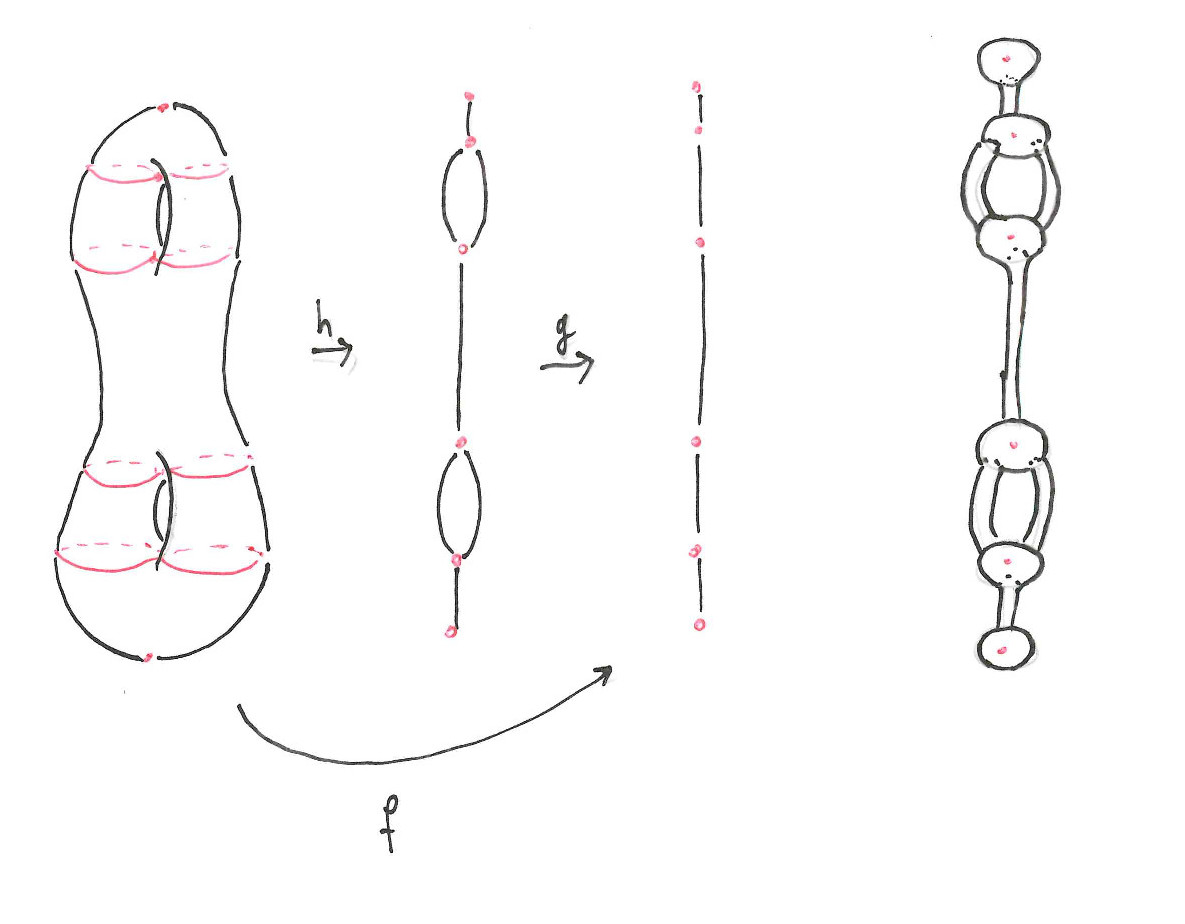
\includegraphics[height=4in]{figures/typicalmorse.jpg}
	\label{fig:typicalmorse}
\end{figure}

\begin{proof}
	Figure \ref{fig:typicalmorse} depicts a typical Morse function acting on the closed oriented surface of genus 2, and samples some of the notation we will define initially.
	We begin by examining the preimages of points $x\in\R$.
	Denote the space $f\inv(x)$ by $\Sigma_x$, a small interval around $x$ by $\varepsilon(x)=(x-\varepsilon,x+\varepsilon)$, and the neighbourhood in $\Sigma$ around $\Sigma_x$ by $f\inv(\varepsilon(x))=\varepsilon(\Sigma_x)$.
	The spaces $\Sigma_x$ and $\varepsilon(\Sigma_x)$ may not be connected, so we index the connected components by superscript.
	Let $p$ be a critical point of $f$ with critical value $f(p)=x$.
	By our assumption that critical values are distinct, $p$ is the only critical point of $f$ in $\Sigma_x$.
	The connected component of $\Sigma_x$ containing $p$ is called the \emph{singular fiber} at $p$ and is denoted $\Sigma_x^p$.
	The connected component of $\varepsilon(\Sigma_x)$ containing $p$ is called the \emph{critical neighbourhood} at $p$ and is denoted $\varepsilon^p(\Sigma_x)$.
	By the regular value theorem, any regular value pulls back through $f\inv$ to a disjoint collection of circles in $\Sigma$ called \emph{regular fibers}.
	Likewise, a neighbourhood $\varepsilon(x)$ that contains no critical values of $f$ pulls back to a disjoint collection of annuli in $\Sigma$.
	The restriction of $f$ to the components of $\Sigma_x$ that do not contain a critical point has $x$ as a regular value, so the remaining connected components of $\Sigma_x$ are all copies of $S^1$ that we index by $\Sigma_x^i$ for $i=1,\dots,k$, and their associated neighbourhoods are the annuli $\varepsilon^i(\Sigma_x)$.
	When referring to an arbitrary connected subspace of $\Sigma_x$ that could be the singular fiber $\Sigma_x^p$ or a regular fiber $\Sigma_x^i$, we will use the notation $\Sigma_x^*$.
	
	The shape of a singular fiber $\Sigma_x^p$ is determined by the index of $p$.
	Because $f$ is a Morse function whose domain is a surface, its critical points are easily classified by the Morse lemma (Lemma \ref{lem:morselemma}).
	Locally in $\Sigma$, a critical point of index 0 is a minimum, of index 1 a saddle, and of index 2 a maximum of $f$.
	
	Let $x$ be a critical value for the critical point $p$ and take $\varepsilon$ to be small enough that $\varepsilon(x)$ contains no critical values other than $x$.
	When $p$ is of index 0 or 2, we can immediately deduce that $\varepsilon^p(\Sigma_x)$ is diffeomorphic to a disc.
	When $p$ is of index 1, the Morse lemma tells us that $\Sigma$ looks like a standard saddle near $p$.
	The intersection of $\Sigma_x^p$ with this saddle is a cross whose centre is $p$.
	For $y\in\varepsilon(x)$, $y$ is a regular value whose preimage is a disjoint union of circles.
	The circles above and below the saddle singularity are the result of smoothing out the cross into a pair of oriented arcs, done in two possible ways.
	The orientations of these circles orient the cross, which has two incoming arms and two outgoing arms which appear in alternating order.
	A Morse function has distinct singular fibers, so the cross we know about in $\Sigma_x^p$ must have its arms connected in $\Sigma_x^p$ through nonsingular orientation--preserving arcs.
	We can then see that $\Sigma_x^p$ is a figure 8, and $\varepsilon^p(\Sigma_x)$ is a pair of pants in $\Sigma$.
	

	\begin{figure}
		\centering
		\caption{Smoothing a cross into a saddle}
		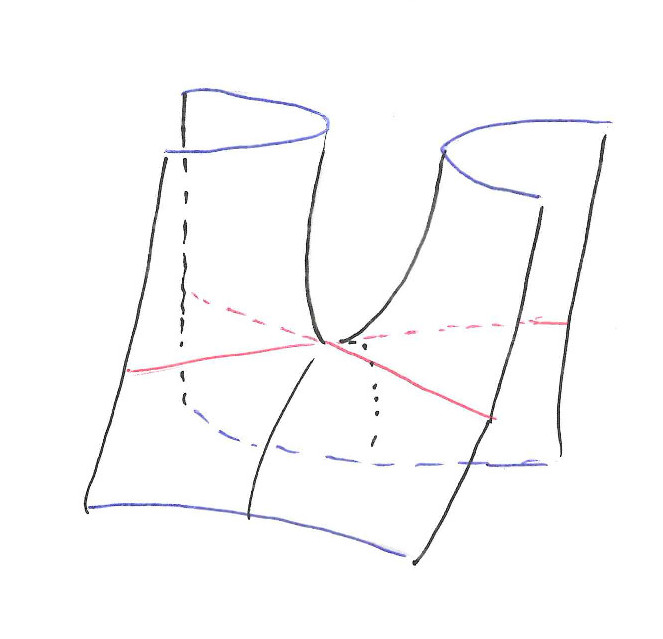
\includegraphics[height=3in]{figures/smoothcross.jpg}
		\label{fig:smoothcross}
	\end{figure}
	
	This analysis is sufficient to form a handle decomposition for a cobordism of $(\Sigma,\emptyset)$.
	We begin with the 3--manifold $\Sigma\times\I$ with boundary components $\Sigma_0=\Sigma\times\{0\}$ and $\Sigma_1=\Sigma\times\{1\}$, and let $f:\Sigma_0\to\I$ be a Morse function with distinct critical values $x_i$.
	The general idea is that we attach handles to $\Sigma_0$, altering that boundary component until it is empty.
	The $x_i$ partition $\I$ into open intervals containing only regular values.
	We take the associated regular annuli to be attaching regions for 3--dimensional 2--handles, and then fill in what remains with 3--dimensional 3--handles.
	
	For an interval $(x_i,x_{i+1})$, consider the subinterval $\varepsilon(t_i)$ where $x_i<t_i<x_{i+1}$ and $\varepsilon$ is small enough that $\varepsilon(t_i)$ contains neither $x_i$ nor $x_{i+1}$.
	Take the associated regular annuli $\varepsilon(\Sigma_{t_i})$ to be the attaching regions for 3--dimensional 2--handles.
	The boundary component that was once $\Sigma_0$ is now the result of removing the interiors of the annuli $\varepsilon(\Sigma_{t_i})$ from $\Sigma_0$ for each $t_i$, and then introducting discs parallel to the cores of the attached 2--handles.
	These discs are seen as $\DD\times\{0\}$ and $\DD\times\{1\}$ inside of a 2--handle $\DD\times\D^1$.
	The boundary circles of the discs are $\Sigma_{t_i-\varepsilon}$ and $\Sigma_{t_i+\varepsilon}$ for each $i$.
	
	There are now intervals about each critical point that we know, from our analysis above, pull back to discs, annuli, and pairs of pants.
	Each of these subsurfaces have circle boundaries that correspond to the regular fibers $\Sigma_{t_i-\varepsilon}$ and $\Sigma_{t_i+\varepsilon}$ which were capped with discs in the previous step.
	The altered boundary described before is therefore a collection of copies of $S^2$, which we take to be the attaching regions of 3--dimensional 3--handles.
	
	With these handles attached, we obtain $(\Sigma\times\I)\cup\{\textrm{2--handles}\}\cup\{\textrm{3--handles}\}$, which is a 3--manifold with exactly one boundary component of $\Sigma_1$, i.e. a cobordism of the pair $(\Sigma,\emptyset)$.
	
	The corresponding dual handle decomposition is realized by turning the process upside down.
	Where we previously had 3--handle attachments with cores $\D^3\times\{\vec{0}\}$ and cocores $\{\vec{0}\}\times\{\vec{0}\}$, we now have 0--handles with cores $\{\vec{0}\}\times\{\vec{0}\}$ and cocores $\D^3\times\{\vec{0}\}$.
	In other words, the dual construction begins by taking the disjoint union of a collection of 3--discs that correspond to the space obtained by capping the boundary circles of the components $\varepsilon(\Sigma_{x_i})$ with 2--discs and then filling the spheres with 3--balls.
	Where we previously had 2--handle attachments with cores $\DD\times\{\vec{0}\}$ and cocores $\{\vec{0}\}\times\D^1$, we now have 1--handle attachments with cores $\{\vec{0}\}\times\D^1$ and cocores $\DD\times\{\vec{0}\}$.
	In other words, we connect the 0--handles together using 1--handles.
	The old belt 0--spheres of the 2--handles in the previous construction correspond here to new attaching 0--spheres, and the attaching maps are chosen to preserve orientability cf.\ Remark~\ref{rmk:1handle}.
	The new attaching 0--spheres bound the new cores, the old core 2--discs are now cocores.
	This construction yields a 3--manifold whose boundary is exactly $\Sigma$, and is indeed another cobordism of the pair $(\Sigma,\emptyset)$.
	
	A Stein factorization $f=g\comp h$ is simple to describe.
	Define the equivalence relation $\sim$ on the points in $\Sigma$ by putting $p\sim q$ if and only if $f(p)=f(q)=x$ and $p$ and $q$ are in the same subspace $\Sigma_x^*$.
	Then $h$ is the quotient map $\Sigma\to \Sigma/\!\!\sim$ where the points of $\Sigma/\!\!\sim$ are the subspaces $\Sigma_x^*$, and $g$ is the map $\Sigma/\!\!\sim\, \to\R$ defined by $g(\Sigma_x^*)=x$.

	The Stein complex $S=\Sigma/\!\!\sim$ can be viewed as a graph $G$.
	A critical value $x=f(p)$ has an associated singular fiber $\Sigma_x^p$ in $S$, and possibly some copies of $S^1$ given by $\Sigma_x^i$.
	We take the associated points $h(\Sigma_x)$ in $S$ for each critical value to be the vertex set $v(G)$.
	For a pair of adjacent critical values $x_{j}$, $x_{j+1}$, an appropriate choice of $\varepsilon$ and $x\in(x_{j},x_{j+1})$ yields a collection of regular annuli $\varepsilon(\Sigma_x)$ in $\Sigma$ that has boundary inside of $\Sigma_{x_{j}}\cup\Sigma_{x_{j+1}}$.
	In $S$, we find $h(\varepsilon(\Sigma_x))$ to consist of 1--dimensional strands that connect components of $\Sigma_{x_{j}}$ and $\Sigma_{x_{j+1}}$.
	The set of pairs $(v,w)$ of connected subspaces with $v\in\Sigma_{x_{j}}$ and $w\in\Sigma_{x_{j+1}}$ such that $v$ and $w$ are connected by a strand in $S$ forms the edge set $e(G)$.
	
	At this point, $G$ corresponds exactly to the dual handle decomposition given earlier.
	For each vertex of $G$ we get a 0--handle.
	For each edge, a 1--handle.
	We attach 1--handles with only one demand: that the resulting space continues to be orientable.
\end{proof}

The Stein complex obtained in the proof of Theorem~\ref{thm:2bound3} may have superfluous vertices.
In particular, a vertex $v$ of $G$ that is adjacent to exactly two verticex $u$ and $w$ via the edges $(u,v)$ and $(v,w)$ may be replaced, along with its adjacent edges, by a single edge $(u,w)$.
To see that the handle decomposition described by this Stein complex graph is equivalent, examine the attaching region of the 1--handle corresponding to $(u,v)$ as it sits inside the boundary of the 0--handle corresponding to $v$.
This region may be isotoped over the 1--handle corresponding to $(v,w)$, where it ends up in the boundary of the 0--handle corresponding to $w$.
We are left with a 0--handle $v$ and 1--handle $(v,w)$ that are contractible into $w$.

\section{3--Manifolds Bound 4--Manifolds}
\label{sec:3bound4}

To extend the results of the previous section to the case of 3--manifolds bounding 4--manifolds, we consider generic proper smooth maps from closed orientable 3--manifolds into the 2--ball $B^2$.
Such a map is Morse--like in the sense that its singular set is well behaved, it can be studied via the same techniques as in Section \ref{sec:2bound3}, and we may recover a Stein factorization and Stein complex that define a handle decomposition for a bounding 4--manifold.

\begin{theorem}
	\label{thm:3bound4}
	Let $M$ be a closed orientable 3--manifold.
	Then a proper generic smooth map $f:M\to \BB$ determines a handle decomposition for a cobordism of the pair $(M,\emptyset)$.
\end{theorem}

\begin{proof}
	By Sard's theorem, the image of the singular set $f(s_f)$ in $\BB$ has Lebesgue measure 0.
	By genericity, and because the maps constructed in Chapter \ref{cha:alg1} satisfy this requirement, we take $s_f$ to consist of a set of arcs in the plane that intersect each other only pairwise and transversally, in such a way that $\BB\setminus s_f$ consists of a collection of regions $R_i$ homeomorphic to copies of $\BB$ along with a single annular region $R_\infty$ that does not intersect $f(M)$, and in such a way that $f(s_f)$ has a natural structure as a simple undirected 4--valent planar graph.
	We classify the critical values of $f$ as codimension 1 inside of arcs away from crossings, and codimension 2 at arc crossings.
	This classification makes the simple undirected planar graph structure of $f(s_f)$ explicit.
	The vertex set is given by the set of codimension 2 critical values and the edge set is the collection of codimension 1 critical values.
	
	We obtain a 4--manifold with boundary $M$ by attaching 2--handles corresponding to the regular regions $R_i$, 3--handles corresponding to codimension 1 singularities, and 4--handles corresponding to codimension 2 singularities.
	
	We will first focus on a region $R$ in $\BB$ that is not $R_\infty$.
	Begin by ``shrinking'' $R$ away from $f(s_f)$ into a space $\D$ that is homeomorphic to $\DD$
	Every point of $\D$ has preimage a disjoint collection of circles by the regular value theorem, so we centre our analysis on an arbitrary regular value $x$ and its regular fibers, where $M_{x,k}$ denotes the $k\nth$ regular fiber mapped over $x$ by $f$.
	An appropriate closed tubular neighbourhood of $M_{x,k}$ will consist entirely of regular fibers that map into $\D$ and has the structure of a closed 2--disc bundle over the circle, hence is a solid torus.
	The neighbourhood can be extended to enclose the entirety of $f\inv(\D)$.
	
	In summary, an arbitrary point $x_i$ is chosen from a closed 2--disc $D_i$ which itself is taken as a shrinking of an open region $R_i$.
	For each $k$, the $k\nth$ regular fiber $M_{i,k}$ over $x_i$ is taken as the zero section of a 2--disc bundle that maps over $D_i$.
	Such a bundle is an open solid torus, and the $k\nth$ bundle is denoted $V_{i,k}$.
	Of particular importance in $V_{i,k}$ are the zero section and a certain isotopy class of longitudes.
	The zero section $z(V_{i,k})$ is a regular fiber that maps over a point interior to $\D_i$, and the longitudinal isotopy class is the one that contains regular fibers that map to single boundary points of $D_i$.
	This pair determines an attaching map for 4--dimensional 2--handle attached over $V_{i,k}$.
	
	\begin{figure}
		\centering
		\captionsetup{justification=centering}
		\caption{Closed sleeve around an arc of codimension 1 critical values and the two neighbouring codimension 2 critical values}
		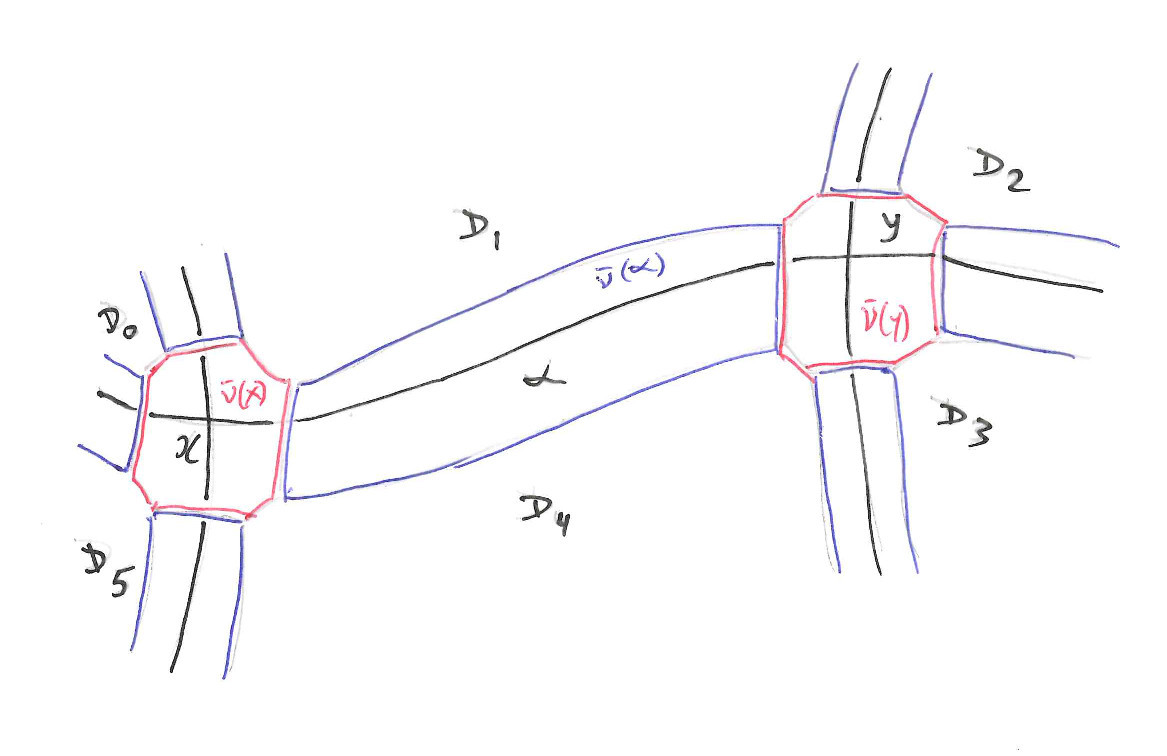
\includegraphics[height=4in]{figures/critsleeve.jpg}
		\label{fig:critsleeve}
	\end{figure}
	
	Consider an arc $\alpha$ of codimension 1 critical values that separates a pair of regions $R_i$ and $R_j$ where either $i$ or $j$ may be $\infty$.
	As when we considered regions, $\alpha$ has been shrunk away from the codimension 2 critical values it connects.
	Let $\nbhd{\alpha}$ be a closed ``sleeve'' around $\alpha$ whose boundary intersects the boundaries of $D_i$ and $D_j$ as in Figure \ref{fig:critsleeve}.
	The restriction of $f$ to the preimage of a linear transversal to $\alpha$ that connects $D_i$ and $D_j$ is, itself, a Morse function.
	The intersection with $\alpha$ is a critical point of this restriction, and the same techniques from the proof of Theorem \ref{thm:2bound3} may be applied to $f\inv(\nbhd{\alpha})$.
	A strand of singular fibers over $\alpha$ consists of an interval in the case of an extremum for the associated Morse function or an interval crossed with the figure 8 when the associated Morse function yields a saddle singularity.
	The critical neighbourhood $f\inv(\nbhd{\alpha})$ contains a connected component that is either $\DD\times\I$ when we have cross sectional extremum, or $P\times\I$, where $P$ is the pair of pants surface, i.e.\ the 2--sphere with three interior 2--balls removed, when the cross section yields a saddle.
	All remaining connected components are intervals crossed with regular annuli.
	We use $A=S^1\times\D^1$, alternatively the 2--sphere with two interior 2--balls removed, to denote an annulus, and find $A\times\I$ to be the form of all remaining connected components.
	
	Whenever one of the regions that $\alpha$ separates is $R_\infty$, the cross section necessarily gives us an extremum, and the critical neighbourhood over $\nbhd{\alpha}$ is $\DD\times\I$.
	We call $\alpha$ a \emph{definite fold} when the critical neighbourhood is $\DD\times\I$, and an \emph{indefinite fold} when the critical neighbourhood is $P\times\I$.
	
	Let $x$ be a codimension 2 critical value and $\nbhd{x}$ the closed neighbourhoods whose boundary agrees with the shrunken regions and arc sleeves it is near as in Figure \ref{fig:critsleeve}.
	The possible singular fibers over $x$ are cataloged in \cite{Saeki}, and Figure \ref{fig:saekising} displays them.
	The singular fibers over $x$ may be disconnected.
	When that is the case, the fibers have the form seen in our codimension 1 analysis.
	Otherwise, the singular fiber has the shape of a 4--valent directed graph.
	The regular fibers are still copies of $S^1$.
	In each case $f\inv(\nbhd{x})$ is a 3--dimensional thickening of the corresponding fibers, hence is a disjoint collection of handlebodies of genus 0,1,2, or 3.
	The neighbourhood of a regular fiber is still a solid torus, so all but at most two of the connected components of $f\inv(\nbhd{x})$ will be genus 1 handlebodies.
	
	\begin{figure}
		\centering
		\captionsetup{justification=centering}
		\caption{Possible singular fibers of a proper generic smooth map from an orientable 3--manifold to a surface}
		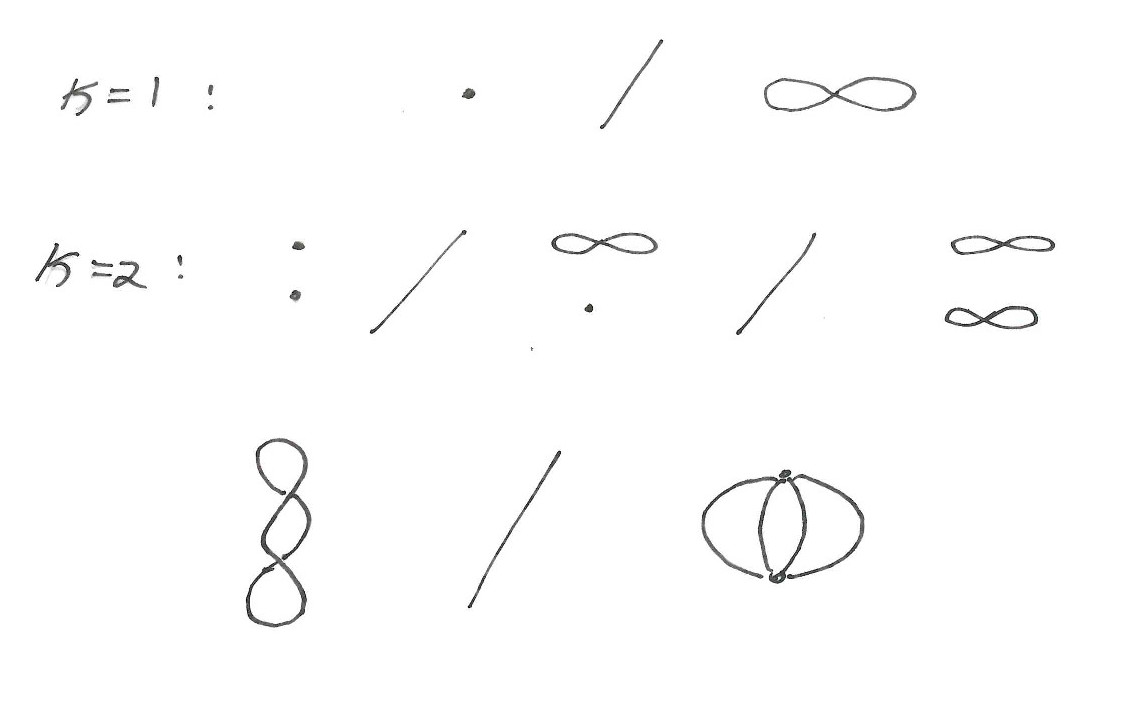
\includegraphics[height=3in]{figures/saekising.jpg}
		\label{fig:saekising}
	\end{figure}
	
	We may now begin describing a handle decomposition for a cobordism $W$ of the pair $(M,\emptyset)$.
	Begin with $M\times\I$, whose boundary is $M_0\sqcup M_1$ with $M_0=M\times\{0\}$ and $M_1 = M\times\{1\}$, and a proper generic smooth map $f:M_0\to\BB$.

	For each $i<\infty$ indexing the connected regions of $\BB\setminus f(s_f)$, we index over $k$ the connected components of $f\inv(R_i)$.
	Consider $D_i\subset R_i$, a 2--disc of regular values, and $V_{i,k}$, the $k\nth$ regular solid torus that maps over $D_i$.
	The solid torus $V_{i,k}$ has a trivial disc bundle structure over the regular fiber $M_{i,k}=z(V_{i,k})$, and $f(M_{i,k})=x$ in the interior of $\D_i$.
	Because we consider a single solid torus for the rest of this argument, we abbreviate $V_{i,k}$ to $V$, $M_{i,k}$ to $z(V)$ and $\D_i$ to $\D$.

	Let's remember what we're doing here --- we're attaching handles in such a way that, once all handles have been attached, the boundary component $M_0$ of $M\times\I$ has been filled in.
	In this step we attach 2--handles over $V$.
	Our goal is to do so in such a way that we remove the ``bad'' solid torus $V$ and replace it with a solid torus that is ``nice,'' where ``nice'' means that the newly introduced solid torus can be filled in by attaching 3-- and 4--handles.
	This happens by deleting $V$ and gluing 2--discs to the longitudes in $\pd V$ that are regular fibers of points in the boundary of $D$.
	To attach a 2--handle over $V$, we need
	\begin{enumerate}
		\item The isotopy class of an embedding $g:S^1\to M_0$, and
		\item the isotopy class of an identification $G:S^1\times\DD\to\nbhd{g(S^1)}$.
	\end{enumerate}
	The embedding $S^1\to M_0$ is easy enough to define as we will just be identifying $S^1$ with $z(V)$.
	This $S^1$ lives as the attaching sphere $S^1\times\{0\}$ inside of the 2--handle $\DD\times\DD$ that we plan to attach.
	Taking $\pd (\DD\times\DD)=(S^1\times\DD)\cup(\DD\times S^1)$ to be the genus 1 Heegard splitting of $S^3$, we will be defining a map $G:V\to S^1\times\DD$, where $S^1\times\DD$ is the first torus component.
	We call the other torus $V^*$.
	In order to satisfy our desired criteria, we need to have $G$ be in the isotopy class of a map that takes a regular fiber $J$ over a point in the boundary of $\D$ to $S^1\times\{1\}$.
	When this is true, we may form the adjunction $(M\times\I)\cup_{G\inv}(\DD\times\DD)$ and $J$ bounds a disc in $V^*$.
	Every fiber in the interior of $V$ now bounds a disc, and the new boundary is exactly $V^*$, whose meridians are the fibers that project over the boundary of $\D$.
	This is the property we wanted --- we've replaced the ``bad'' solid torus $V$ with the ``nice'' solid torus $V^*$.
	
	\begin{figure}
		\centering
		\captionsetup{justification=centering}
		\caption{The solid tori $V$ and $V^*$ with boundary curves $J$, $K$, and $L$.}
		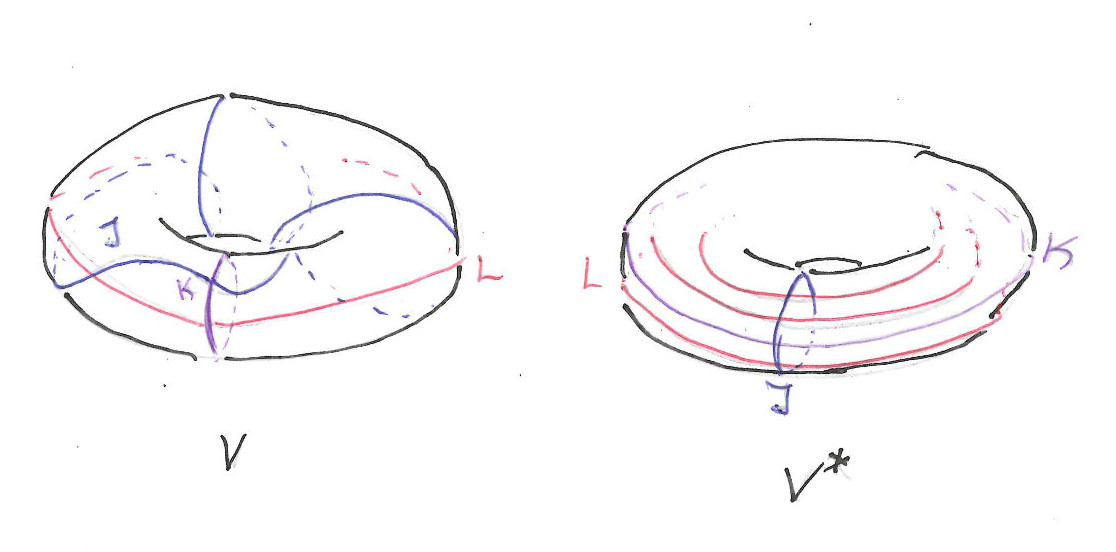
\includegraphics[width=6in]{figures/VV.jpg}
		\label{fig:VV*}
	\end{figure}
	
	A class $[G]$ satisfying the above is unique and it exists.
	To see why, let $\varphi:V\to S^1\times\DD$ be any trivialization of $V$, take $K=\varphi\inv(\{1\}\times S^1)$ to represent the meridinal isotopy class of $V$, and take $L$ be the longitude in $\pd V$ defined by $L=\varphi\inv(S^1\times\{1\})$.
	Let $J=f\inv(q)$ in $\pd V$ represent the isotopy class of regular fibers over boundary points of $\D$, where $q$ is an arbitrary point in the boundary of $D$.	
	Figure \ref{fig:VV*} shows the curves $J$, $K$, and $L$ with orientations sitting on $\varphi(V)$.
	Thinking of $S^1\times\DD$ as a subset of $\C^2$ gives it a natural orientation, which we have pulled back through $\varphi$ onto $K$ and $L$.
	We give $J$ a compatible orientation so that its intersections with $K$ and $L$ can be counted.
	Put $\kappa$ to be the oriented intersection number of $J$ and $L$.
	Then $\varphi(J)\in \pd\varphi(V)$ is in the isotopy class of $h_M^{\kappa}(\varphi(L))$, where $h_M$ is the meridinal twist defined in Theorem \ref{thm:mpgV}.
	Take $G=H_M^{-\kappa}\comp\varphi$, where $H_M$ is the extension of $h_M$ to the solid torus defined in Remark \ref{rmk:2handle}.
	In the boundary of $G(V)$, $G(J)$ is in the isotopy class of $S^1\times\{1\}$, $G(K)$ is in the isotopy class of $\{1\}\times S^1$, and $G(L)=h_M^\kappa(S^1\times\{1\})$.
	Existence of $G$ is shown, and uniqueness up to isotopy comes from the same uniqueness in trivializations of $V$ and of $H_M$.
		
	With 2--handles attached, we move onto the preimages of arc sleeves.
	Let $\nbhd{\alpha}$ be an arc sleeve, and consider the connected components of $f\inv(\nbhd{\alpha})$.
	Figure \ref{fig:arcsleevepre} displays the possible connected components of arc sleeve preimages, each of which has the form of a surface crossed with the interval.
	The boundary circles of these surfaces at a cross section $\Sigma\times\{t\}$ project through $f$ over the boundaries of shrunken regions, so they are filled with discs that sit inside of attached 2--handles from the previous step.
	In each case, we obtain a copy of $S^2\times\D^1$ over which we attach a 3--handle.
	The further modification to $M_0$ that takes place when we attach 3--handles can be thought of as the deletion of a copy of $S^2\times D^1$ followed by gluing 3--discs over the newly created 2--sphere boundary components.
	
	\begin{figure}
		\centering
		\captionsetup{justification=centering}
		\caption{Possible connected components of arc sleeve preimages}
		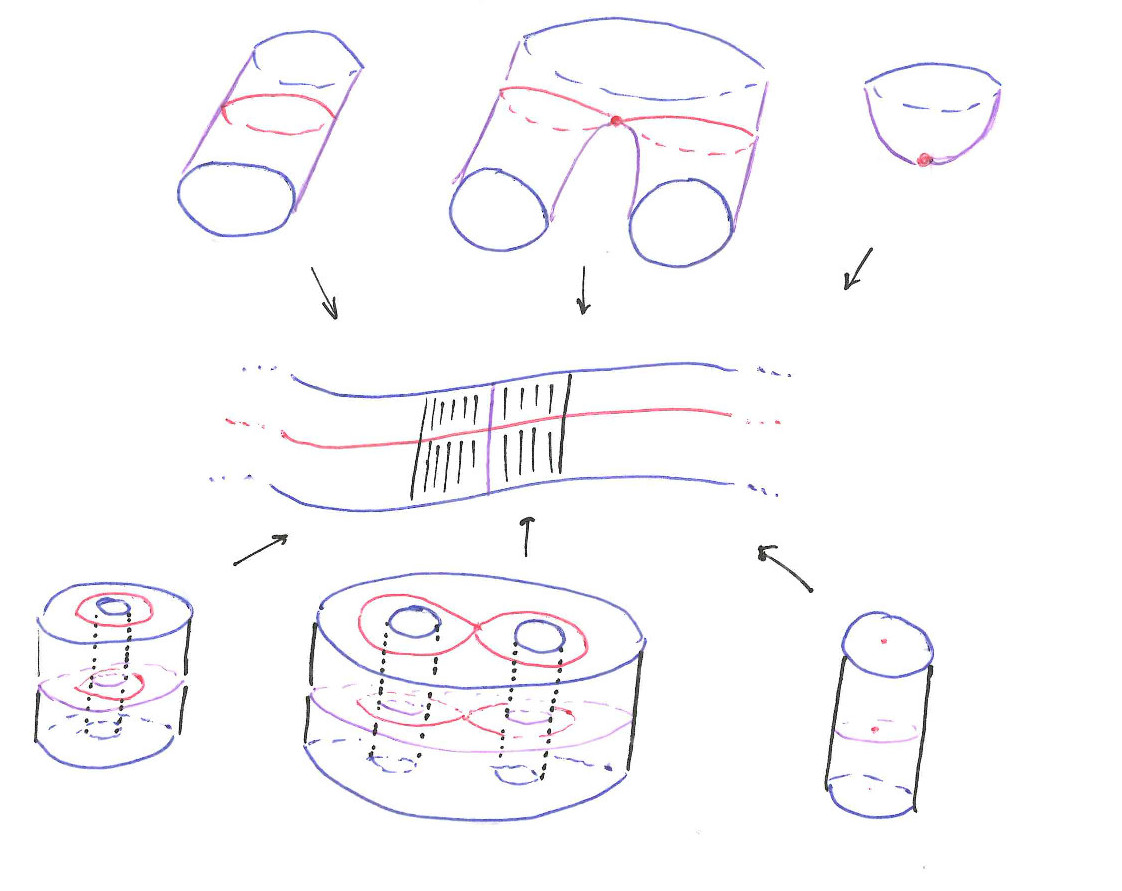
\includegraphics[height=4in]{figures/arcsleevepre.jpg}
		\label{fig:arcsleevepre}
	\end{figure}
	
	Finally, let $x$ be a codimension 2 critical value and let $\nbhd{x}$ be its sleeve.
	We find $x$ at the crossing of a pair of strands of codimension 1 critical values, and those strands are classified as definite or indefinite folds.
	The analysis of the codimension 2 critical value is then broken down into five cases.
	In four cases, we are able to extend the codimension 1 situation.
	This happens when the singular fiber is disconnected, called an \emph{uninteractive} singular fiber, or when one of crossing folds is definite.
	When both folds are indefinite and the singular fiber is connected, then the singular fiber is called \emph{interactive} and we defer to the analysis in \cite{CostThur08}.
	
	First we look at the connected components of $f\inv(\nbhd{x})$ that do not contain a singular fiber over $x$.
	These connected components are made from regular fibers, i.e.\ circles, that project over $\nbhd{x}$, i.e. a 2--disc.
	As in the case of regions of regular values, they are solid tori $V_{x,k}$, using the same naming convention that has been established for solid tori that map over the regions $D_i$.
	Seeing $V_{x,k}$ as a 2--disc bundle over $f\inv(x)$, we can find an isotopy class of longitudes that project over single points in the boundary $\pd\nbhd{x}$.
	These longitudes bound discs introduced during 2-- and 3--handle attachment.
	The union of all such discs yields a solid torus $V_{x,k}^*$ in the boundary.
	The boundary component consisting of $V_{x,k}$ and $V_{x,k}^*$ is described by the Heegaard splitting $V_{x,k}\cup_\varphi V_{x,k}^*$ where $\varphi$ takes a longitude of $V_{x,k}$ to a meridian of $V_{x,k}^*$.
	This is the standard genus 1 Heegaard splitting of $S^3$, so we have a copy of $S^3\times\D^0$ over which we may attach a 4--handle.

	The component that comes from an uninteractive definite fold is of the form $\DD\times\I$ as in the case of codimension 1 critical values.
	The 2--sphere boundary of this shape is filled with 2--discs from our 2-- and 3--handles, so this shape is the adjunction of a pair of 3--discs glued over their boundary.
	This is the genus 0 Heegaard splitting of $S^3$, so we have a copy of $S^3\times\D^0$ over which we may attach a 4--handle.
		
	\begin{figure}
		\centering
		\caption{Destabilizing pairs for the pair of pants}
		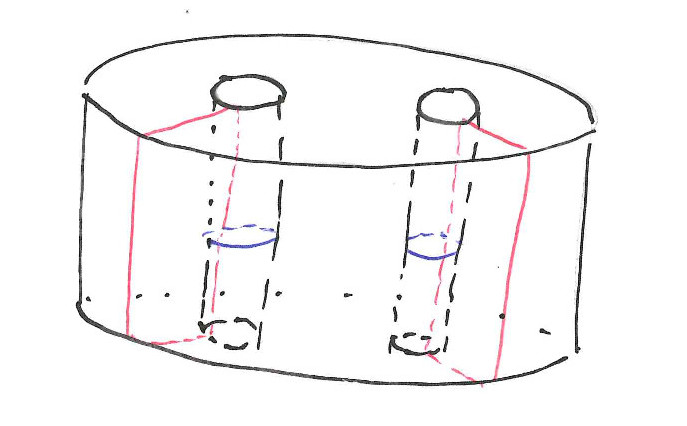
\includegraphics[height=3in]{figures/destabpants.jpg}
		\label{fig:destabpants}
	\end{figure}
		
	An uninteractive singular fiber that comes from an indefinite fold is the figure 8, and the preimage $f\inv(\nbhd{x})$ is a closed tubular neighbourhood of the figure 8 graph, which is homeomorphic to the pair of pants crossed with an interval.
	Here, we find a Heegaard splitting of genus 2 with two destabilizing pairs, showing that the splitting is a splitting of $S^3$, and we can attach a 4--handle to it by Theorem \ref{thm:lilwald}.
	An appropriate choice of meridians in $f\inv(\nbhd{x})$ would be a pair of curves that run from cuff to waist along the inside of each of the legs in the pair of pants, crest the waist, then down the outside of the legs back to the cuff.
	Meridians for the solid filled by our 2-- and 3--handles would run around the cuffs of each leg.
	Figure \ref{fig:destabpants} illustrates the idea.
	
	When an indefinite and definite fold interact, we get the same shapes found in the case of an uninteractive definite fold.
	From a 1--dimensional Morse function viewpoint, we witness a homotopy of a pair of peaks separated by a saddle come together into a single peak, eliminating the saddle.
		
	This leaves us with the case of interacting indefinite folds.
	The full analysis is covered in Section 4.4 of \cite{CostThur08}.
	They show that filling in $f\inv(\pd\,\nbhd{x})$ with 2--discs and gluing the two genus 3 handlebodies together over $f\inv(\pd\,\nbhd{x})$ results in a Heegard splitting of $S^3$ by explicitly finding 3 destabilizing pairs.
	We attach 4--handles over these 3--spheres.
	Attaching a 4--handle over a 3--sphere fills in the 3--sphere with a 4--disc, so these final modifications completely eliminate what is left of $M_0$.
	We are left with a handle decomposition for a cobordism of the pair $(M,\emptyset)$ built on top of $M_0$ in $M\times\I$.
\end{proof}

Let $f:M:\to\BB$ be a proper generic smooth function and $W$ a the cobordism of the pair $(M,\emptyset)$, both as per the construction in Theorem \ref{thm:3bound4}. 
Because the handle decomposition produced for $W$ consists of handles of index 2,3, and 4, the associated dual decomposition contains handles of degree 0,1, and 2.
Our goal is to obtain a combinatorial description of this decomposition, and we find this through the Stein complex.

Recall that the Stein complex for a Morse function on a surface was given by a 1--complex.
In the case of a proper generic smooth map $M\to\BB$, the Stein complex is given by a 2--complex $S$.
The vertices of $S$ correspond to 0--handles, the edges to 1--handles and the 2--cells to 2--handles.

We define the Stein factorization and complex of $f$ as usual.
Let $\sim$ be an equivalence relation on $M$ defined by $p\sim q$ if and only if $f(p)=f(q)=x$ and $p$, $q$ are in the same connected component of $f\inv(x)$.
Then $f=g\comp h$ where $h$ is the quotient map $M\to M/\!\!\sim$ and $g$ takes a point in $f\inv(x)$ to $x$.

\begin{theorem}
	\label{thm:stein2complex}
	Let $f$, $M$, $S$, and $W$ be as we defined above.
	Then $S$ is a 2--dimensional CW--complex that embeds flatly in $W$.
\end{theorem}

\begin{proof}
	There are only a few locations where $S$ could fail to be a CW--complex, and those are found over the critical values of $f$.
	We construct $S$ as we would any other CW--complex, by iteratively attaching cells of increasing dimension, and define a map $\varphi:S\into W$ that is almost a flat embedding in a similar fashion.
	Let $S$ be empty and begin by adding 0--cells to $S$.
	
	For a codimension 2 singular value $x$ of $f$, the fibers of over $x$ were discussed in Theorem \ref{thm:3bound4}.
	The Stein factorization $f=g\comp h$ has $h$ crush each fiber to a point, which we take as a new 0--cell in $S$.
	Let $\nbhd{x}$ be a sleeve of $x$ as in Theorem \ref{thm:3bound4}.
	In the construction of $W$, we attached 4--handles over 3--spheres with Heegaard decompositions over $f\inv(\nbhd{x})$.
	The cocore of a 4--handle is a single point, so we associate the 0--cells of $S$ with the cocores of 4--handles in $W$.
	Let $x_i$ be a fiber over $x$, let $H_i^4\subset W$ be the 4--handle associated to $x_i$, let $c_i\in H_i^4$ be the cocore of $H_i^4$, and let $v_i$ be the vertex of $S$ associated to $x_i$.
	Define $\varphi(v_i)=c_i$.
	
	We can now add edges to $S$.
	Let $\alpha$ be an open strand of codimension 1 critical points of $f$ with $\pd\overline\alpha=\{x,y\}$, a pair of codimension 2 critical points of $f$.
	Pulling back $\alpha$ to $M$ yields an open interval crossed with the fibers over any point of $\alpha$ and pulling back $\overline\alpha$ connects the fibers over $x$ and $y$.
	For a fiber $\alpha_i$ over $\alpha$ with endpoints $\alpha_i^x$ sitting inside of a fiber over $x$ and $\alpha_i^y$ sitting in a fiber over $y$, we add an edge attached over the vertices $v_i^x$ and $v_i^y$ associated to the fibers over $x$ and $y$.
	This corresponds to the action of $h$ on $\alpha_i$, which crushes the interval of fibers to an interval.
	
	Let $\nbhd{\alpha}$ be a sleeve of $\alpha$ as in Theorem \ref{thm:3bound4}.
	To construct $W$ we attached 3--handles over copies of $S^2\times\D^1$, those $S^2\times\D^1$ contained copies of $\Sigma\times\D^1$ with $\Sigma$ the 2--sphere with one, two, or three open 2--balls removed, and those $\Sigma\times\D^1$ projected over $\nbhd{\alpha}$.
	The cocore of a 3--handle is a copy of $\D^1$, which corresponds to an edge in $S$.
	Let $\alpha_i$ be a fiber over $\alpha$, $H_i^3$ the 3--handle associated with $\alpha_i$, $c_i$ the interval cocore of $H_i^3$, and $e_i$ the edge of $S$ corresponding to $\alpha_i$ with $\pd e_i=\{u,v\}$.
	Because $e_i$ is a 1--cell, it is homeomorphic to an interval $[\,0,1\,]$, so we take a slightly smaller closed subinterval $e_i'$ in $e_i$ (just as we can take $[\,\varepsilon,1-\varepsilon\,]$ inside of $[\,0,1\,]$) and define $\varphi(e_i')=c_i$.
	The endpoints of $c_i$ are the belt sphere of $H_i^3$, and they intersect the 4--handles $H_u^4$ and $H_v^4$ corresponding to $u$ and $v$.
	The intersection points are in the boundary 3--spheres of these 4--handles, so there are straight lines inside of the 4--handle that connect the cocore to these boundary points.
	Define $\varphi$ on $e_i\setminus e_i'$ to be those straight line segments in the appropriate continuous way.
	
	And finally, the 2--cells.
	Let $R$ be an open ball of regular values in the plane, and let $D$ be the 2--disc inside of $R$ that pulls back through $f$ to a disjoint collection of solid tori over which we attached 2--handles in our construction of $W$.
	Let $H$ be the 2--handle attached over a solid torus $V$ projecting over $D$.
	The boundary of $H^2$ is a 3--sphere with genus 1 Heegaard splitting consisting of $V$ and a dual torus $V^*$.
	We attached $H^2$ because we wanted to fill the boundary of $V$ with 2--discs that were easy to attach 4-- and 3--handles over, and $V^*$ is also contained in the union of these 4-- and 3--handles.
	The vertices and edges of $S$ corresponding to this collection 4-- and 3--handles forms a cycle $C$ in the 1---skeleton of the Stein complex already built.
	We know that $R$ contains only regular values, so it pulls back to a disjoint collection of open solid tori.
	Let $U$ be the open solid torus in this collection with $f(U)=R$ and $V\subset U$.
	In particular, $\pd V=\pd V^*\subset U$.
	The fibers of $S$ are fibers of $f$ that project over the regular values in $R$, so $h(U)$ is a 2--ball.
	The closure of $U$ intersects the singular fibers corresponding to the 4-- and 3--handles that contain $V^*$.
	We take $h(U)$ in $S$ to be a 2--cell attached over $C$.

	To define $\varphi$ on the 2--cell $\sigma_U$ corresponding to $U$, we start by defining it on $\sigma_V$, a subdisc of $\sigma_U$ (cf.\ the case of defining $\varphi$ on the edges of $S$, where $\sigma_V\subset\sigma_U$ just like how $\{z\in\C:|z|^2\leq 1-\varepsilon\}\subset\DD$).
	Recall that	$H^2$ is the 2--handle attached over $V$.
	It is useful to think of $H^2$ as a $\DD$ bundle over $\DD$, where the base space and zero section are the cocore $C_V$ of $H^2$.
	We define $\varphi(\sigma_V)=C_V$, and then examine the intersection of $C_V$ with the 4-- and 3--handles of $W$.
	The collection of higher index handles that intersect $H^2$ is exactly the collection that contains $V^*$, and the intersection is exactly $V^*$.
	The cocore $C_V$ intersects $V^*$ in exactly the belt sphere of $H^2$.
	We then extend $\varphi$ to $\sigma_U\setminus\sigma_V$ exactly as we did with the edges of $S$, by connecting the belt sphere of $H^2$ with the cocores of the 4-- and 3--handles by line segments.
	
	This demonstrates first that the Stein complex $S=h(M)$ has the structure of a 2--complex.
	Secondly, the map $\varphi:S\into W$ constructed here is piecewise--linear where it is not smooth, so can be smoothed into a flat embedding of a CW--complex.											
\end{proof}

In Section \ref{sec:proj} it is convenient to remove open balls from a given 3--manifold $M$ and build a projection of $M'$ instead.
We want the results of this section to still apply, so we state this in Theorem \ref{lem:stillworks}

\begin{lem}
	\label{lem:stillworks}
	Let $M$ be a closed orientable 3--manifold, and let $M'$ be $M$ with a finite number of disjoint 3--balls removed.
	Call the disjoint 2--sphere boundary components of $M'$ by $pd_i M'$.
	Let $f:M'\to\DD$ be a proper generic smooth map such that $f(\pd M')$ is a disjoint collection of intervals in the boundary of $\DD$ and the image of the singular set of $f$ away from $\pd M'$ is as described in the proof of Theorem \ref{thm:3bound4}.
	Then the Stein complex recovered for $f$ in the manner of Theorem \ref{thm:stein2complex} is exactly the Stein complex recovered for an extension of $f$ to $M$.
\end{lem}

\begin{proof}
	The singular fibres near $f(\pd M')$ are all definite folds, and extending $f$ to 3-balls attached over the boundary components of $M'$ yields an extension of that definite fold over the image of the 3--ball.
\end{proof}

All that's left is to realize the Stein complex as a set of instructions to build a handle decomposition of $W$, dual to the one obtained in Theorem \ref{thm:3bound4}, that relies only on $f$ and $S$.
We state this more precisely in Theorem \ref{thm:3stein4}.

\begin{theorem}
	\label{thm:3stein4}
	Let $f$, $M$, $S$, $W$ be as defined above.
	Then there exists a 4--manifold $W^*$ that is a cobordism of the pair $(M,\emptyset)$ in which $S$ embeds flatly as in Theorem \ref{thm:stein2complex}, and this manifold may be reconstructed from the combinatorics of $S$ and the map $f$.
\end{theorem}

\begin{proof}
	Let $G$ be the 1--skeleton of $S$.
	We consider first the 4--handlebody obtained by attaching to $\emptyset$ a 4--dimensional 0--handle $H_v^0$ for each vertex $v$ of $G$, embedding $v$ as the core of $H_v^0$, attaching a 1--handle $H_e^1$ with orientation preserving attaching maps into $\pd H_u^0$ and $\pd H_v^0$ for each edge $e=(u,v)$ of $G$, embedding $e$ as the core of $H_e^1$ plus a pair of line segments to the cores $\pd H_u^0$ and $\pd H_v^0$.
	The result is a 4--dimensional handlebody called the \emph{4--thickening} of $G$, and is denoted by $H_4(G)$.
	
	Consider now $U_S(G)$, a closed regular neighbourhood of $G$ in $S$.
	This is equivalent to $S$ minus an open ball inside of each 2--cell (as in Theorem \ref{thm:stein2complex} when we considered $\sigma_U\setminus\sigma_V$), or can also be seen as $G$ plus an annulus attached by one of its boundary components over each cycle that a 2--cell was attached over in Theorem \ref{thm:stein2complex}.
	In either case, $U_S(G)$ collapses onto $G$ and the 4--thickening of $U_S(G)$ is homeomorphic to the 4--thickening of $G$.
	To build $W$, we make a 3--thickening of $U_S(G)$, and then a 4--thickening of the 3--handlebody obtained.
	This time, however, we pay attention to how the 2--cells of $S$ interact with the thickening.
	
	We built $S$ to have a 1--skeleton $G$ whose interior vertices are all of degree 4 and whose boundary vertices are all of degree 3.
	The 3--thickened regular neighbourhoods of the five possible vertex types and the three possible edge types in $S$ are depicted in Figure \ref{fig:3thickeningblocks}.
	We use these to build the 3--thickening $H_3(U_S(G))$ of $U_S(G)$ where $U_S(G)$ is embedded in $H_3(U_S(G))$ and intersects the boundary of $H_3(U_S(G))$ in the curves depicted on the blocks in Figure \ref{fig:3thickeningblocks}.
	Thinking of $H_3(U_S(G))$ as generically a bundle of $\II$ over $U_S(G)$, the curves would be the zero section of the bundle over the boundary of $U_S(G)$.
	Once we have $H_3(U_S(G))$, there is a unique orientable $\II$ bundle over $H_3(U_S(G))$, and this is the 4--thickening of $G$.
	This bundle can be obtained either by specifying local trivializations that reverse the orientation of the $\II$ factor along the curves in $H_3(U_S(G))$ along which the space becomes nonorientable, or by first building the 3--thickening of $T\subset G$, a maximal spanning tree of $G$, 4--thickening that space, and then attaching all remaining 1--handles in the unique orientation preserving way.
	We choose the second construction.
	
	\begin{figure}
		\centering
		\captionsetup{justification=centering}
		\caption{3--thickening blocks for the 1--skeleton of the Stein complex}
		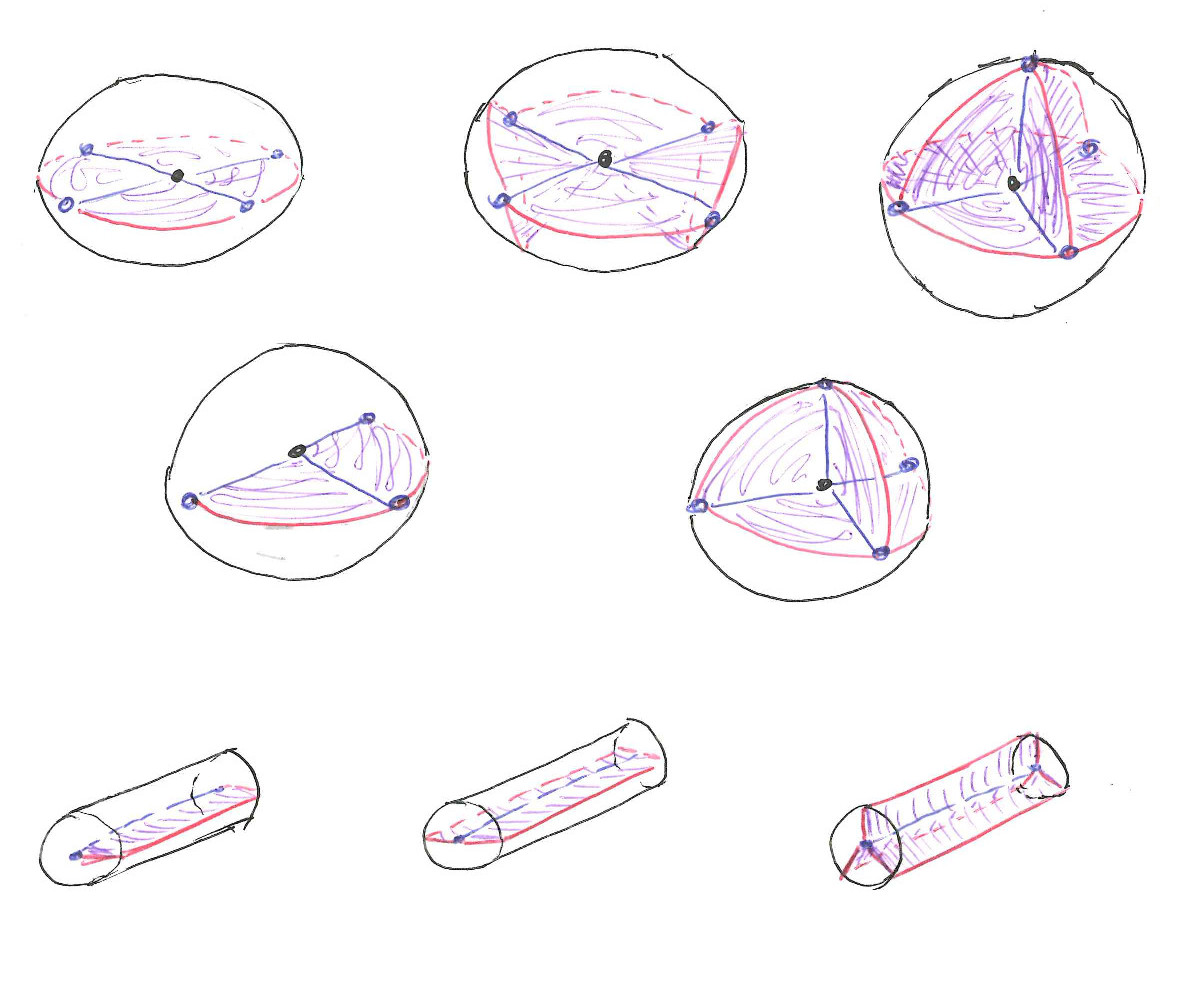
\includegraphics[width=6in]{figures/3thickeningblocks.jpg}
		\label{fig:3thickeningblocks}
	\end{figure}
	
	Building $H_3(U_S(T))$ by adding an appropriate vertex block to $H_3(U_S(T))$ for each vertex of $T$, then connect them together with edge blocks in the unique way that is forced by the combinatorics of $S$ for each edge of $T$.
	Take the product of this space with $\II$.
	The result is a $\II$--bundle over $H_3(U_S(T))$ and generically a $\II^2$--bundle over $U_S(T)$.
	To extend this to $G$, we add 1--handles for each edge in $G$ that is not in $T$.
	Every such edge has at least one 2-handle in $S$ attached over it, and every 2--cell of $S$ attaches over at least one edge added in this step.
	We use the product of our edge blocks with $\II$ as the 4--disc structure for our 1--handles.
	The combinatorics of $S$ and the requirement that $H_4(U_S(G))$ is orientable make these handle attachments unique.
	Our 4--thickening $H_4(U_S(G))$ is once again a $\II$--bundle over $H_3(U_S(G))$ and generically a $\II^2$--bundle over $U_S(G)$.
	The boundary circles of $U_S(G)$, corresponding to 2--cells of $S$ and thus 2--handles of $W$, are now thickened to solid tori in $H_4(U_S(G))$.
	The last step to this construction is the attachment of 2--handles over these solid tori. 
	
	Let $v^*$ be a boundary circle of $U_S(G)$ corresponding to a 2--cell $c_v$ of $S$ with thickening $V^*$ in the boundary of $H_4(U_S(G))$.
	The first thing we must do is specify a canonical 0--framing on $V^*$, which we do by investigating the diagonal of the square fibers $\II$.
	As a subspace of $V^*$, the union of the fibers have the structure of an annulus or a M\"obius strip.
	To see which we get, we turn to the completion of $H_4(U_S(T))$ into $H_4(U_S(G))$ accomplished by attaching 4--dimensional 1--handles.
	At least one such 1--handle corresponded to an edge of $\pd c_v$, and $n$ of them were attached with an orientation reversal in both $\II$ factors.
	If $n$ is even then the diagonal is an annulus and we put the canonical 0--framing as the trivialization that takes one boundary component of that annulus to $S^1\times\{1\}$.
	If $n$ is odd then the diagonal is a M\"obius strip.
	In this case we take a curve that follows one half of the boundary component of the M\"obius strip (i.e. once around $V^*$ in the longitudinal direction along the boundary), then connects to itself via one half positive twist in the orientation of $V^*$ (which is canonically oriented by the canonical orientations of the double intervals $\II$).
	
	With a 0--framing specified, we just need framing coefficients.
	To recover those, we ask how our canonical framing sits inside of $M$.
	This question is well defined because the solid tori we are attaching 2--handles over are the $V^*$ we examined in the proof of Theorem \ref{thm:3bound4}, and the boundaries of these tori are contained in $M$.
	
	The complex $S$ embeds flatly into $W$, and the restriction of that embedding to the 0-- and 1--handles of $W$ is exactly how $U_S(G)$ embeds in $H_4(U_S(G))$.
	Specifically, the zero section of the torus $V^*$ above is the belt sphere of the 2--handle in $W$ corresponding to the 2--cell $c_v$ in $S$.
	This belt sphere is then the attaching sphere of the dual 2--handle in the handle decomposition of $W^*$ and the framing coefficient is then the number of meridinal twists from the 0--framing to the longitude in $V^*$ that is a meridian of $V$.
	Attaching a 2--handles over every such $V^*$'s yields a handle decomposition of a 4--manifold $W^*$ that is dual to the decomposition of $W$ acquired in Theorem \ref{thm:3bound4}.
	We conclude that $W^*$ is the desired cobordism of $(M,\emptyset)$.
\end{proof}

There are a couple of points left to address in this chapter.
The first is that of explicitly recovering the 0--framing curve used in the attachment of 2--handles in Theorem \ref{thm:3stein4}, a necessity for turning this process into an algorithm.
The second is an acknowledgment of the origin of the ideas in this Section.

The 0--framing $L$ is a curve in the shared boundary of $V$ and $V^*$ that is a number of meridinal twists of $V^*$ away a meridian of $V$.
This number is the framing coefficient we equip to the 2--cell of $S$ representing 2--handle attachment over $V^*$ in the construction of $W^*$.

Because $L$ is a longitude of $V^*$, it wraps exactly once around the meridinal direction of $V$, and can thus be realized as a section over $\pd \D$ where $f(V)=\D$.
Let $\D_0$ be the zero section of $V$ as a disc bundle over an interior regular fiber of $V$.
Then the oriented intersection number of $J$ with $D$ yields the framing coefficient.
We compute the framing coefficient for a 2--cell of $S$ in Section \ref{sub:gleams} using this method.


This work is based on that of Costantino and Thurston in \cite{CostThur08} and of Turaev in \cite{Turaev91}.
Theorem \ref{thm:3stein4} in particular is a version of the Turaev Reconstruction Theorem.
Three distinct versions can be found as Theorem 4.1 of \cite{Cost05}, 3.8 of \cite{CostThur08}, and 19.1 of \cite{Turaev91}.
The proof presented is closest in form to that found in \cite{Cost05}.
These selections offer a decent introduction to the theory of shadows of 4--manifolds.
A shadow is a 2--complex with extra structure, and the Stein complex found in this section is almost a shadow.

%\section{Shadows of 3-- and 4--Manifolds}
%\label{sec:shadow}

The building instructions mentioned in the previous section were studied by Turaev in ~\cite{Turaev91} and are called \emph{shadows}.
Shadows are piecewise--linear 2--dimensional structures that live inside of piecewise--linear, compact, oriented 4--manifolds.
The central algorithm of this work uses shadows of 3-- and 4-- manifolds to construct a triangulation of a 4--manifold with a given 3--manifold boundary.

\begin{defn}
  Let $P$ to be a compact topological space.
  If every point $p$ of $P$ has a neighbourhood homeomorphic to an open set in one of the following local models
  \begin{enumerate}
    \item the closed 2--disc $D^2$,
    \item the product of the interval $I=[0,1]$ with the $Y$--shaped graph $K_{1,3}$, or
    \item the cone on the complete graph $K_4$,
  \end{enumerate}
  then $P$ is a \emph{simple polyhedron}.
  \{ FIGURE HERE DEPICTING THE LOCAL MODELS\}
  The set of points which do not have a neighbourhood homeomorphic to an open set in $D^2$ form a 4--valent graph which we call the \emph{singular set} of $P$ and denote by $\Sing (P)$.
  The vertices and edges of $\Sing (P)$ are called the vertices and edges of $P$.
  We call the connected components of $P\setminus\Sing (P)$ the \emph{regions} of $P$.
  
  The local models each have boundary.
  Being a surface, the 2--disc has a well defined boundary.
  In the local model $K_{1,3}\times I$, the boundary consists of the set $(K_{1,3}\times \{0\})\cup (K_{1,3}\times \{1\})\cup (V(K_{1,3})\times I)$, where $V(K_{1,3})$ denotes the vertex set of the graph $K_{1,3}$.
  The boundary points of the cone on $K_4$, defined at $K_4\times I /\sim$, where $\sim$ is defined to be $(x,1)\sim (y,1)$ for any $x,y$, are the points in $K_4\times \{0\}$.
  
  If a point $p$ of $P$ has a neighbourhood homeomorphic to an open set containing a point in the boundary of one of our three local models, then $p$ is a \emph{boundary point} of $P$.
  The set of all boundary points of $P$ is the boundary of $P$ and is denoted by $\pd P$.
  A region of $P$ is \emph{internal} if its closure is disjoint from $\pd P$.
  If $\pd P$ is empty then $P$ is \emph{closed}.
\end{defn}

Simple polyhedra are almost shadows.
To define a shadow, we need to consider simple polyhedra embedded in a 4--manifold.
First, we introduce a concept from simple--homotopy theory.

\begin{defn}
  Let $K$ be a simplicial complex, and let $\tau$, $\sigma$ be simplices so that $\dim \sigma$ is maximal, $\dim\tau=\dim \sigma -1$, and no simplex of dimension $\dim \sigma$ other than $\sigma$ contains $\tau$.
  We obtain the complex $L$ from $K$ by removing $\sigma$ and $\tau$.
  That is, $L= K\setminus(\inter{\sigma}\cup\tau)$.
  We say that $L$ is an \emph{elementary collapse} of $K$.
  
  If a complex $L$ is obtained from $K$ through iterated elementary collapses, then we say that $L$ is a \emph{simplicial collapse} of $K$.
  We may also say that $K$ {\em collapses} onto $L$.   
\end{defn}

We are finally ready to define a shadow.

\begin{defn}
  Let $W$ be a piecewise--linear, compact, oriented 4--manifold.
  Let $P\subset W$ be a closed simple sub--polyhedron of $W$ such that $W$ collapses onto $P$ and the regions of $P$ are \emph{locally flat} in $W$.
  That is to say, if $p$ is in $P\setminus\Sing(P)$ then there is a chart $(U,f)$ of $W$ around $p$ so that $f(P\cap U)$ is contained in $\R^2\subset \R^4$.
  We define $P$ to be a \emph{shadow polyhedron} of $W$.
\end{defn}

\begin{rmk}
  There is a notion of shadow equivalence in~\cite{Turaev91} via basic shadow moves.
  A shadow polyhedron whose regions are all homeomorphic to discs is called \emph{standard}, and through Turaev's shadow moves any shadow polyhedra can be made standard.
  Furthermore, the algorithms which make up the bulk of this document produce a standard shadow polyhedron, so from here forward we always consider our polyhedra to be standard.  
\end{rmk}

Not every piecewise--linear, compact, oriented 4--manifold contains a shadow polyhedron.
A necessary and sufficient condition for the existence of a shadow polyhedron in such a 4--manifold is the existence of a handle decomposition of $W$ containing no handles of index greater than 2, as shown in~\cite{Turaev91}.
This requirement tells us that $W$ has a connected non-empty 3--manifold boundary $M$.
A shadow is defined for $M$ as well.

\begin{defn}
  A shadow polyhedron of an oriented, closed 3--manifold $M$ is a shadow polyhedron $P$ of a compact 4--manifold $W$ with $\pd W=M$
\end{defn}

This gives us the following theorem for free.

\begin{theorem}
  \label{the:shadowexistence}
  Every closed, oriented 3--manifold has a shadow polyhedron.
\end{theorem}

\begin{proof}
  To sketch the proof, we use the results of Lickorish and Kirby as summarized in~\cite{GompStip}.
  Any closed, oriented smooth 3--manifold $M$ has a presentation as integral surgery over a link $L$ in $\sthr$.
  A handle decomposition of a 4--manifold with boundary equal to $M$ can be obtained from the integral surgery diagram of $M$.
  We begin with a 0--handle, which is just a copy of $B^4$ with boundary $S^3$.
  We put our surgery presentation in this $S^3$.
  Each component of the surgery link in $S^3$ will be the attaching sphere of a 2--handle, and the integer surgery coeffifient will be the element of $\pi_1(\gl{2}{\R})$ that fully describes the framing of this 2--handle.
  Adding a 2--handle over every component of the link results in a 4--manifold $W$ such that $\pd W=M$.
 
  The link diagram also determines the shadow of $W$ hence of $M$.
  Take $\pi:L\to \DD$ to be a regular projection.
  That is, $\pi$ is injective everywhere except for at a finite number of points which coincide with the crossings of $L$.
  Then the mapping cylinder $(I\times L)\coprod \DD/(0,x)\sim\pi(x)$ with a disc glued to the free link ends at $\{1\}\times L_i$ is, as per our definition, a shadow of $W$.
\end{proof}

It is natural to wonder how closely related shadows are with their associated 3-- and 4--manifolds.
Just as simple--homotopy type is not a complete invariant of 4--manifolds, a shadow polyhedron does not uniquely determine a 4--manifold.
The following example demonstrates this explicitly and hints at what kind of additional information is needed to uniquely identify a shadow with a 4--manifold.

\begin{ex}
  \label{ex:polypoly}
  We examine disc bundles over $\stwo$.
  Take $W_0$ to be the trivial disc bundle $\D^2\times S^2$ and $W_1$ to be the bundle whose 0--section has self--intersection number of 1 in the ambient 4--manifold.
  Each $W_i$ collapses onto $\stwo$, so each have shadow $\stwo$.
  Because $W_0$ is $\D^2\times S^2$, it's boundary is $S^1\times S^2$.
  One can see that $W_1$ has handle decomposition with exactly one 0--handle $B^4$ and one 2--handle attached over the unknot in $S^3=\pd B^4$ with framing coefficient 1.
  This manifold is a punctured $\CP^2$, so has boundary $S^3$.
  We've defined a shadow polyhedron of an oriented, closed 3--manifold $M$ to be a shadow polyhedron $P$ of a compact 4--manifold $W$ with $\pd W=M$, so $S^3$ and $S^2\times S^1$ each have shadow polyhedron $S^2$.
\end{ex}

We've found a pair of distinct 4--manifolds with distinct boundaries, but the shadow of each is $S^2$.
We want to construct a 4--manifold whose boundary is a given 3--manifold, and this shows that we need more than just a naked shadow polyhedron to do so.
The information needed is carried by the internal regions of a polyhedron and are named ``gleams'' by Turaev.
One can intuit from the Example~\ref{ex:polypoly} that a ``gleam'' might describe the regular neighbourhood of an embedded shadow.

\begin{defn}
  Let $P$ be a polyhedron embedded in the 4--manifold $W$ in a locally flat way.
  Then there exists a canonical colouring of the internal regions of $P$ by elements of $\frac{1}{2}\Z$ called \emph{gleams}.
  A gleam necessarily depends on the embedding of $P$.
  We may also discern a canonical colouring of the internal regions of $P$ by elements of $\Z_2$ called the $Z_2$--\emph{gleam} that depends only on the combinatorial structure of $P$.
  The $Z_2$--gleam of a region of $P$ determines whether the gleam of that region is an integer or half--integer.

  Let $D$ be an internal region of $P$.
  Because $P$ is assumed to be standard, we know that $D$ is an open disc and the closure of $D$ is a closed disc.
  The embedding of $D$ in $P$ extends to an embedding $e : \bar{D} \to P$ so that $e$ takes $\pd\bar{D}$ into $\Sing(P)$.
  Denote by $U(D)$ the simple polyhedron that is a small open regular neighborhood of $D$ in $P$.
  We may construct $U(D)$ from $\bar{D}$ by first gluing the core of either an annulus or M\"obius strip, to $\pd\bar{D}$.
  Then, for each point $p$ of $\pd\bar{D}$ so that $e(p)$ is a vertex of $P$, let $A_p$ be an arc in the band attached to $\pd\bar{D}$ so that $A_p$ intersects the core of the band only at $p$.
  Obtain $U(D)$ by gluing half the boundary of a disc to $A_p$ for each $p$.
  The map $e$ extends easily to the map $e':U(D)\to P$.
  Define the $\Z_2$--gleam of $D$ in $P$ to be equal to $1$ if the band attached to $\pd\bar{D}$ was a M\"obius strip and $0$ if the band was an annulus.
  
  \{FIGURE: $U(D)$ FOR $Z_2$--GLEAM EVEN AND ODD\}
  
  Now, suppose that $f:P\to W$ is our locally flat embedding of $P$ and let $D, \bar{D}, e: D \to P, U(D)$ and $e'$ be defined as before.
  Because $e'$ embeds $U(D)$ in $P$, we consider $U(D)$ to be a subset of $P$.
  A regular neighbourhood of $f(U(D))$ in $W$ collapsing onto $f(U(D))$ is an oriented 4--ball $B^4$.
  Let $p_0$ be a point in $\pd\bar{D}$ and $(V,g)$ a chart of $W$ with $V$ containing $p_0$ such that the intersection $V_P = V\cap f(U(D))$ is contained in $f(U(D))$.  
  The embedding $f$ is locally flat, so $g(V_P)$ is contained in a 3--dimensional slice $B^3$ of $g(V)$ and $g(f(\bar{D})\cap V)$ is contained in a 2--dimensional slice of $B^3$.
  If $p_0$ is not a vertex of $P$, then there are exactly two other regions $D'$ and $D''$ of $P$ that meet $D$ at $p_0$.
  The direction in $B^3$ in which $D'$ and $D''$ separate away from $p_0$ can be extended to a direction in $g(V)$ where it is an element of the projective line $P^1$ of lines orthogonal to $f(D)$ sufficiently close to $f(p_0)$.
  If $p_0$ is a vertex of $P$, then ignoring the region of $P$ that meets $D$ only at $p_0$ leaves two suitable separating regions that meet $D$ at $p_0$.
  We form a smooth bundle of directions over $\pd\bar{D}$ which is a section of a $P^1$ bundle over $\pd\bar{D}$.
  The obstruction to extend this section to all of $D$ is a class of $H^2 (D, \pd D; \pi_1 (P^1 ))$.
  The ambient space $g(V)$ is oriented so $D$ is oriented.
  The class of $H^2 (D, \pd D; \pi_1 (P^1 ))=\Z$ is an integer $z$ that corresponds to the number of times a section of the boundary of $D$ loops around a $P^1$ bundle, which is the number of half loops made around a $S^1$ bundle.
  We are interested in the $S^1$ bundle, so we take the gleam of $D$ to be $z/2$.
  Note that $z$ modulo 2 is exactly the $\Z_2$--gleam of $D$.
\end{defn}

\begin{theorem}\cite{Turaev91}
  \label{the:turaevreconstruction}
    Let $S$ be a polyhedron whose internal regions are equipped with gleams.
    Then there exists a canonical construction associating to $S$ the a pair $(W,S)$, where $W$ is a piecewise--linear, compact, oriented 4--manifold $W$ containing an embedded copy of $S$ with shadow $S$ can be reconstructed from the combinatorics of $S$.
\end{theorem}

We can extend our definition of shadows to shadows of pairs $(M,G)$ where $M$ is a 3--manifold whose boundary is not necessarily empty and $G$ is an embedded framed graph whose vertices have degree either 1 or 3.
This extension is useful because it allows us to build a shadow for a closed 3--manifold from a reasonable decomposition into blocks whose shadows are known.
In this case, the polyhedron representing our shadow will have boundary and the 1--cells of the boundary will be classified.

\begin{defn}
  Define a \emph{boundary--decorated} standard polyhedron to be a standard polyhedron $P$ with boundary so that $\pd P$ is a graph whose edges are coloured one of $i$ for internal, $e$ for external, or $f$ for false.
  The graph $\pd P$ then has three distinct subgraphs $\pd_i P$, $\pd_e P$ and $\pd_f P$ intersecting only at vertices and whose union is $\pd P$.
  If $\pd_f P=\emptyset$ then we call $P$ as \emph{proper}.
\end{defn}

Boundary decorated polyhedra can be turned into a shadows for a 3--manifolds with boundary and with framed graphs embedded in their interior.
The boundary of the 3--manifold is represented by the subgraph $\pd_e P$ and the embedded graph is represented by the subgraph $\pd_i$.

\begin{defn}
  Let $P$ be a boundary decorated standard polyhedron properly embedded in a 4--manifold $W$ so that $W$ collapses onto $P$ with a framing on $\pd_i P$.
  An embedding $f:X\to Y$ is \emph{proper} if $f(\pd X) = f(X)\cap \pd Y$ and $f(X)$ is transverse to $\pd Y$ everywhere in $\pd X$.
  
  Let $M$ be the complement of an open regular neighbourhood of $\pd_e P$ in $\pd W$ and let $G$ be a framed graph embedded in $M$ whose core is $\pd_i P$.
  Then $P$ is a \emph{shadow} of the pair $(M,G)$.
  If the false boundary is empty, then $P$ is a \emph{proper} shadow of $(M,G)$.
  Gleams are defined on the interior regions of $P$ as before.
\end{defn}





\chapter{Projections and initial data}
\label{cha:projection}
\label{cha:alg1}

A gleamed shadow of a 3-manifold M is a shadow of a 4-manifold bounded by M.
The ultimate goal of this thesis is to provide an algorithm that takes as input an edge-distinct triangulation $T$ of the closed orientable 3--manifold $M$ and produces as output a triangulation of a 4--manifold $W$ such that $\pd W$ is equivalent in the sense of triangulations to $T$.
This algorithm is split into three chapters.
Chapter \ref{cha:projection} builds a piecewise--linear Morse 2--function $T\to\RR$ and collects all data from that function necessary to build a gleamed shadow shared by $T$ and a 4--manifold bounded by $T$.
Chapter \ref{cha:shadow} builds a gleamed shadow from the information obtained in \ref{cha:projection}.
Chapter \ref{cha:manifold} assumes we have a gleamed shadow $(S,\glm)$ and constructs a triangulated 4--manifold whose shadow is $(S,\glm)$.

The data we are trying to collect and retain with the algorithms of this chapter are as follows:
\begin{enumerate}
  \item A list of polygons which we will call regions.
  \item A colouring of every edge of every region using one of the three colours $i,f,h$.
  \item A wedge number of $0$, $1$, or $2$ for any edge coloured $i$.
  \item A list of adjacencies between regions.
        An item in this list consists of a pair of regions and an $i$--coloured boundary edge of each region.
  \item A list of piecewise--linear circles associated to each region.
        An item in this list is an ordered list of polygonal 2--cells which live in a closed polyhedral 3--complex so that any two consecutive 2--cells lie on the boundary of the same 3--cell, yet any 3--cell contributes either zero or two 2--cells to any given list.  This list is indexed by the list of regions in item 1.
\end{enumerate}
This data is sufficient to build a shadow, as seen in Chapter \ref{cha:shadow}.


\section{Preliminaries}
\label{def:preliminaries}
Before beginning the algorithm, we should establish some properties of piecewise--linear maps from polyhedra to $\RR$.
These properties are called upon to support some algorithms in this chapter.
We also review the basics of planar graphs, as these are the objects that encode the information we wish to carry to Chapter~\ref{cha:alg2}.

\begin{defn}
	\label{def:planargraph}
	Let $G$ be a connected graph such that an embedding of $G$ in $\RR$ exists.
	Fix $p:G\to\RR$ to be such an embedding.
	Then the pair $(G,p)$ is called a \emph{planar graph}.
	The image $p(G)$ separates $\RR$ into path connected components called the \emph{regions} of $(G,p)$.
	There is exactly one region of $(G,p)$ which is unbounded in the plane, and whose boundary is a cycle of $G$.
	This region, its boundary cycle and all edges and vertices in that boundary cycle are said to be \emph{outer}.
	All other other regions, vertices and edges are \emph{inner}.
	Regardless of the choice of embedding $p$, every chordless cycle of $G$ is the boundary of exactly one inner region of $(G,p)$, and every inner region of $(G,p)$ is bounded by exactly one chordless cycle of $G$, so the inner regions and chordless cycles of $(G,p)$ are in $1$--$1$ correspondence.
\end{defn}

\begin{defn}
	\label{def:stdproj}
	Let $T$ be a tetrahedron with the four vertices $u$, $v$, $w$, $x$, six edges $uv$, $uw$, $ux$, $vw$, $vx$, $wx$, and faces $\hat{u}$, $\hat{v}$, $\hat{w}$, $\hat{x}$, where a face is named by the vertex of $T$ it does not contain.
	Define a projection $\pi: T \to\DD$ by first choosing a map from the vertices of $T$ to distinct points in $\sone$.
	Each point $p$ of $T$ is decribed by the convex combination
	\[
		p = t_u u + t_v v + t_w w + t_x x
	\]
	with the $t_*$ nonnegative and summing to 1.
	We can define $\pi$ at $p$ by
	\begin{eqnarray}
		\label{affine_extension}
		\pi(p)
		&=&
		\pi(t_u u + t_v v + t_w w + t_x x) \nonumber \\
		&=&
		t_u \pi(u) + t_v \pi(v) + t_w \pi(w) + t_x \pi(x)
	\end{eqnarray}
	  
	Without loss of generality, we assume that the points $\pi(u),\pi(v),\pi(w),\pi(x)$ are ordered in a clockwise orientation about $\sone$.
	We call $\pi:T\to\DD$ a \emph{linear tetrahedral projection}.
\end{defn}

\begin{defn}
	\label{def:projpttypes}
	A point of $\DD$ in the image of $\pi$ is one of five types:
	\begin{enumerate}
		\item The four points of type 1 are the images of the vertices of $T$ under $\pi$.
		\item The single point of type 2 is the intersection $\pi(uw)\cap\pi(vx)$.
		\item All points in $\pi(uv)\cup\pi(vw)\cup\pi(wx)\cup\pi(xu)$, excluding the points of type 1, are of type 3.
		\item All points in $\pi(uw)\cup\pi(vx)$ excluding the points of type 1 or 2 are of type 4.
		\item The points of type 5 are the points outside of the image of any vertex or edge of $T$.
	\end{enumerate}
	The image of the $1$--skeleton of $T$ forms a planar graph $G$ inside of $\DD$ whose vertex set consists of the points of types 1 and 2 and whose edges consist of points of type 3 and 4.
	The planar graph embedding cuts the plane into five connected regions: four inner regions that contain all points of type 5, and and one outer region.
	This graph has four outer edges, consisting of the points of type 3, and four inner edges, consisting of the points of type 4.
	
	By definition, the preimage of a point of type 1 is a vertex of $T$.
	The preimage of the single point of type 2 is a line segment between the edges $uw$ and $vx$ interior to $T$.
	A point of type 3 is the image of exactly one point in an edge of $T$.
	A point of type 4 is in the image of exactly one edge and one face, so the preimage of one of these points is a line segment interior to $T$ between those two facets.
	Finally, points of type 5 are in the image of exactly two faces of $T$, and pull back to line segments interior to $T$ between those two faces.
\end{defn}


\section{Build a projection}
\label{alg:proj}
Before beginning the algorithm, we should establish some properties of piecewise--linear maps from polyhedra to $\RR$.
These properties are called upon to support some algorithms in this chapter.
We also review the basics of planar graphs, as these are the objects that encode the information we wish to carry to Chapter~\ref{cha:alg2}.

\begin{defn}
Let $G$ be a connected graph such that an embedding of $G$ in $\RR$ exists.
Fix $p:G\to\RR$ to be such an embedding.
Then the pair $(G,p)$ is called a \emph{planar graph}.
The image $p(G)$ separates $\RR$ into path connected components called the \emph{regions} of $(G,p)$.
There is exactly one region of $(G,p)$ which is unbounded in the plane, and whose boundary is a cycle of $G$.
This region, its boundary cycle and all edges and vertices in that boundary cycle are said to be \emph{outer}.
All other other regions, vertices and edges are \emph{inner}.
Regardless of the choice of embedding $p$, every chordless cycle of $G$ is the boundary of exactly one inner region of $(G,p)$, and every inner region of $(G,p)$ is bounded by exactly one chordless cycle of $G$, so the inner regions and chordless cycles of $(G,p)$ are in $1$--$1$ correspondence.
\end{defn}

\begin{defn}
\label{def:stdproj}
Let $T$ be a tetrahedron with the four vertices $u$, $v$, $w$, $x$, six edges $uv$, $uw$, $ux$, $vw$, $vx$, $wx$, and faces $\hat{u}$, $\hat{v}$, $\hat{w}$, $\hat{x}$, where a face is named by the vertex of $T$ it does not contain.
Define a projection $\pi: T \to\DD$ by first choosing a map from the vertices of $T$ to distinct points in $\sone$.
Each point $p$ of $T$ is decribed by the convex combination
\[
  p = t_u u + t_v v + t_w w + t_x x
\]
with the $t_*$ nonnegative and summing to 1.
We can define $\pi$ at $p$ by
\begin{eqnarray}
\label{affine_extension}
  \pi(p)
  &=&
  \pi(t_u u + t_v v + t_w w + t_x x) \nonumber \\
  &=&
  t_u \pi(u) + t_v \pi(v) + t_w \pi(w) + t_x \pi(x)
\end{eqnarray}
  
Without loss of generality, we assume that the points $\pi(u),\pi(v),\pi(w),\pi(x)$ are ordered in a clockwise orientation about $\sone$.
We call $\pi:T\to\DD$ a \emph{linear tetrahedral projection}.
\end{defn}

\begin{defn}
\label{def:projpttypes}
A point of $\DD$ in the image of $\pi$ is one of five types:
\begin{enumerate}
  \item The four points of type 1 are the images of the vertices of $T$ under $\pi$.
  \item The single point of type 2 is the intersection $\pi(uw)\cap\pi(vx)$.
  \item All points in $\pi(uv)\cup\pi(vw)\cup\pi(wx)\cup\pi(xu)$, excluding the points of type 1, are of type 3.
  \item All points in $\pi(uw)\cup\pi(vx)$ excluding the points of type 1 or 2 are of type 4.
  \item The points of type 5 are the points outside of the image of any vertex or edge of $T$.
\end{enumerate}
The image of the $1$--skeleton of $T$ forms a planar graph $G$ inside of $\DD$ whose vertex set consists of the points of types 1 and 2 and whose edges consist of points of type 3 and 4.
The planar graph embedding cuts the plane into five connected regions: four inner regions that contain all points of type 5, and and one outer region.
This graph has four outer edges, consisting of the points of type 3, and four inner edges, consisting of the points of type 4.

By definition, the preimage of a point of type 1 is a vertex of $T$.
The preimage of the single point of type 2 is a line segment between the edges $uw$ and $vx$ interior to $T$.
A point of type 3 is the image of exactly one point in an edge of $T$.
A point of type 4 is in the image of exactly one edge and one face, so the preimage of one of these points is a line segment interior to $T$ between those two facets.
Finally, points of type 5 are in the image of exactly two faces of $T$, and pull back to line segments interior to $T$ between those two faces.
\end{defn}

Our algorithm begins by defining a projection $\pi:T\to\RR$ satisfying some properties that are very similar to the properties of a smooth Morse 2--function.
We demand first that if we restrict $\pi$ to any tetrahedron $\tet$ of $T$, then $\restr{\pi}{\tet}$ is an affine--linear tetrahedral projection.
Next, let $E,E'$ be edges of $T$ and $\pi(E),\pi(E')$ their images.
From the first condition it is guaranteed that if $\pi(E)\cap\pi(E')$ is nonempty then it consists of the single point $z$.
We demand that if $z$ is interior to $\DD$ then it is in the image of no other edge of $T$ through $\pi$.

The first requirement can be met by choosing arbitrary images for the vertices of $T$, then extending to a linear tetrahedral projection on each tetrahedron as in Equation \ref{affine_extension}.
An arbitrary placement of the $m$ vertices of $T$ does not, however, guarantee the second condition.
Choosing as images for the vertices odd $n\nth$ complex roots of unity (with $n\geq m$) does guarantee this condition by a theorem in \cite{PoonRub98}.
Line segments between vertices of a regular polygon in the plane are called \emph{diagonals}.
The theorem places a bound on the number of diagonals that can intersect at a point.
If the polygon has an odd number of vertices, then this bound is two.

To see how we use this theorem, let $T$ be our input triangulation, and let $|T^0|=m$.
Put an arbitrary ordering on the elements of $T^0$.
Let $n$ be the least odd number greater than or equal to $m$.
Define $\pi(v_k)=e^{2\pi i k/n}$ for every $v_k$ in $T^0$.
Extend $\pi$ over all of $T$.
Then $\pi:T\to\RR$ satisfies our desired properties.


\section{Obtain a planar graph}
\label{alg:planar}

We construct here a planar graph $(G,p)$ from the projection $\pi:T\to\RR$ that will be used throughout this chapter.
The projection $\pi:T\to\RR$ defined in the previous section maps vertices of $T$ to the $n\nth$ roots of unity, where $n$ is odd.
The construction of $(G,p)$ here is essentially an extension of the construction seen in Definition \ref{def:projpttypes} to the whole of $T$.

Every vertex $v$ of $T$ has a distinct image $\pi(v)$ in $\sone$, so our graph $G$ begins with these points as its vertex set $V$.
The vertex of $G$ associated to $v$ in $T$ will be named $G(v)$.
To fill the rest of the vertex set $V(G)$, we examine the images of each pair of non--adjacent edges of $T$ for interior intersections.
Here, edges in $T$ are adjacent if they share a vertex.
For a pair of non--adjacent edges $E$, $F$ of $T$ with boundary vertices $\pd E = v_E\cup w_E$ and $\pd F = v_F\cup w_F$, we may determine whether the line segments $\pi(E)$ and $\pi(F)$ in the plane intersect by checking the order in which the points $\pi(v_E)$, $\pi(w_E)$, $\pi(v_F)$, and $\pi(w_F)$ occur around $\sone$.
Each of these points is at an $n\nth$ root of unity, so there is an obvious ordering that assigns each of these points to an integer.
If $\pi(v_E)$ and $\pi(w_E)$ or $\pi(v_F)$ and $\pi(w_F)$ are adjacacent in this ordering, then $\pi(E)$ and $\pi(F)$ do not intersect.
Otherwise, $\pi(E)$ and $\pi(F)$ intersect.
Each intersection of this type adds a vertex to $V(G)$ which we will name $G(E, F)$ and these are all of the vertices we get.

To make $G$ a planar graph, we need to fix an embedding $p:G\to\RR$.
For a vertex $G(v)$ directly associated with the vertex $v$ of $T$, we define $p(G(v))=\pi(v)$.
For a vertex $G(E,F)$ associated to the intersection of $\pi(E)$ and $\pi(F)$ in the plane, we define $p(G(E,F))=\pi(E)\cap\pi(F)$.
This embedding is chosen so that an edge $e=uv$ of $G$, all of which will be added next, can be embedded in the plane as the line segment connecting $p(u)$ and $p(v)$.

Every edge of $G$ comes from an edge of $T$, and every edge of $T$ produces at least one edge of $G$.
If an edge $E$ of $T$ has image $\pi(E)$ that intersects no other image $\pi(F)$ with $E$, $F$ non--adjacent in $T$, then $E$ adds exactly one edge to $E(G)$ whose vertices are $G(v_E)$ and $G(w_E)$.
Otherwise, $\pi(E)$ intersects the line segments $\pi(E_j)$ for each of the edges in $\{E_j\}_{j=1}^m$ with $E_j$ not adjacent to $E$ in $T$.
In this case, we have a vertex $G(E,E_j)$ in $V(G)$ for each $j$, and $p(G(E,E_j))$ is the point of intersection between $\pi(E)$ and $\pi(E_j)$.
The edges we add to $G$ from $E$ form a path $P$ in $G$ with tails $G(v_E)$ and $G(w_E)$ that passes through every $G(E,E_j)$, and all we need to know is the order in which the vertices occur in $P$.
When this is known, we populate $P$ with edges.

To determine the order of the vertices of $P$, we assume that $\pi(E)$ is a vertical line segment, which is done without loss of generality.
For this discussion, $E$, $\{E_j\}_{j=1}^m$ are as above.
Then
\[
  \pi(v_E)=e^{2\pi i k/n}\text{ and }\pi(w_E)=e^{2\pi i k/n}.
\]
and
\[
  \pi(v_{E_j})=e^{2\pi i p/n}\text{ and }\pi(w_{E_j})=e^{2\pi i q/n}.
\]
Then the $x$--co-ordinate of the intersection $\pi(E)\cap\pi(E_j)$ is fixed at $\cos(2\pi k/n)$, and the $y$--co-ordinate $y_j$ can be found to be
\[
  y_j = \frac{\sin(2\pi i \frac{q-p}{n}) + (\sin(2\pi i \frac{p}{n}) - \sin(2\pi \frac{q}{n}))\cos(2\pi \frac{k}{n})}{\cos(2\pi i \frac{p}{n})-\cos(2\pi i \frac{q}{n})}.
\]
We may compute and order the real numbers $y_j$.
This orders the $v_j$ in the path $P$ from $w_E$ to $v_E$.
This ordering is given by the permutation $\sigma\in \Sigma_m$, so we populate $P$ with the edges $(w_E,\sigma\inv(1))$, $(\sigma\inv(i),\sigma\inv(i+1))$ for $i\in\{1,\dots,m-1\}$, and the edge $(\sigma\inv(m),v_E)$.
We perform this process for each edge of $T$.
As stated above, $p$ is defined on an edge $e=uv$ of $G$ as the line segment between $p(u)$ and $p(v)$.
We then have our planar graph $(G,p)$.

A particularly nice property of a planar graph is that it has well--defined regions, and those regions are in one--to--one correspondence with the chordless cycles of the graph.
Further, there exist standard algorithms to find all chordless cycles in a graph that we may use to find all regions of our planar graph.
We do not include the details of such algorithms here.

\{A FIGURE WOULD BE GREAT HERE\}


%\section{Piecewise--linear maps from polyhedra to $\RR$}
%


%A line $L$ in the plane that contains none of $p$, $q$, $r$, $s$ separates the plane into two connected components and partitions $\{p,q,r,s\}$ into two sets.
%If a partition contains:
%\begin{enumerate}
%  \item the empty set, then the preimage of $L\cap\pi(T)$ pulls back to the empty set.
%  \item a set with one element, then the preimage of $L\cap\pi(T)$ pulls back to a normal triangle in $T$.
%  \item a set with two elements, then the preimage of $L\cap\pi(T)$ pulls back to a normal quadrilateral in $T$.
%\end{enumerate}



%\section{Find all chordless cycles}
%This algorithm finds all chordless cycles in a planar graph $G$.
The algorithm is common.
Delete all vertices of degree at most one.
Repeat this until there are no vertices of degree at most one.
Begin at an arbitrary vertex $v$ and compute all chordless cycles passing through that vertex.
This is easily done by a breadth first search away from $v$.
In a planar graph, the number of chordless cycles passing through $v$ is bounded above by the degree of $v$.
Delete $v$.
Repeat this algorithm until the graph is empty.


\section{Find all mapping triangles}
\label{alg:trilist}

This algorithm takes as input a region $R$ of $G$, represented by chordless cycle $C$ in $G$, and gives as output a list of piecewise--linear circles in the triangulation $T$ that map to a generic point interior to the region $R$ bounded by $C$.
A piecewise--linear circle is unambiguously described as an ordered list of triangles $\{t_i\}$ in $T$ so that every consecutive pair of triangles are from the same $\tet$, and so that every $\tet$ of $T$ represented by a triangle in this list is represented by exactly two triangles in this list.
The piecewise--linear circle is then formed by connecting the centres of consecutive triangles with line segments.

The projection $\pi$ maps the triangle $t$ of $T$ to the triangle $t'$ in $\DD$ so that the vertices $u'$, $v'$, $w'$ of $t'$ are all in $\sone$, and the edges of $t'$ are straight line segments between the vertices of $t'$.
Now $t'$ splits $\DD$ into four path-connected regions: one region which is the image of $t$ and three regions which are not.
Intuitively, take a point $p$ in the disc and a point $q$ in $\sone$ with $q\neq u',v',w'$.
A straight line from $p$ to $q$ crosses $0$, $1$, or $2$ edges of $t'$.
In the case of $0$ or $2$ crossings, $p$ is not in the image of $t$.
If there is exactly $1$ crossing, then $p$ is in the image of $t$.

To implement this into a graph algorithm, recognize that the edges $e_i$ of $t$ map through $\pi$ to paths $P_i$ in $G$.
To check if a given region, represented by the chordless region $C$, is in the image of $t$ we first check whether every vertex of $C$ is in a path $P_i$.
If this is true then we are done --- $R$ is in the image of $t$.
Otherwise, there is a vertex $v$ of $C$ which is not in any $P_i$.
If $v$ is an outer vertex of $G$, then $R$ is not in the image of $t$.
Otherwise, $v$ is in the image of exactly two edges of $T$, and we choose one of those edges arbitrarily.
That edge maps through $\pi$ to the path $P$ whose tail vertices are each outer.
At least one tail vertex, call it $x$, is not a tail of any $P_i$ as otherwise $P$ would be some $P_i$, and this contradicts the statement that $v$ is not in any $P_i$.

Now we have a graph representation of our intuitive understanding of the situation.
The path from $v$ to $x$ represents a straight line segment connecting a point in the disc to a point on the boundary different from a vertex of our triangle.
This is evident by our construction of $G$.
We need only count the number of vertices that $P$ shares with the paths $P_i$.
If exactly $1$ vertex is shared, then the region $R$ is in the image of $t$.
Otherwise, $R$ is not in the image of $t$.


\section{Find all mapping circles}
\label{alg:circlist}
This algorithm takes as input a region of $R$ of $G$ and gives as output a set of lists of triangles in $T$.
Each list unambiguously defines a piecewise-linear circle in $T$ built from line segments between the centres of consecutive triangles.

Take as input a region $R$ of $G$ and build from $R$ a list $L$ of triangles using the above algorithm: \ref{alg:trilist}.
We partition $L$ into sublists corresponding to the connected components of the preimage of a generic point of $R$.
To separate a connected component, we examine a sublist generated from any given triangle of $L$.
Begin by adding an arbitrary triangle $t$ to a sublist $l$ of $L$.
The triangle $t$ is inside exactly two tetrahedra of $T$, so we choose one of these tetrahedra, $S$, arbitrarily.
Now $S$ contains exactly one other $t'$ of $L$, which itself is inside of another tetrahedron $S'$ of $T$.
We add $t'$ to $l$ and continue this process with $S'$ until we find ourselves back at $t$.
Reduce $L$ to $L'=L\setminus l$, and continue until $L^{(n)}$ is empty.
Each sublist $l$ defines a piecewise--linear circle in $T$.
\{FIGURE: A PL CIRCLE\}


\section{Count wedge numbers}
\label{alg:countwedge}

In the previous section, we built lists of circles that map through $\pi$ over the regions of $(G,p)$.
What we do not yet have is a way of describing the fibers of $\pi$ that map over the edges of $(G,p)$.
For an edge $e$ of $(G,p)$ with $p(e)$ in the image $\pi(E)$ for $E$ an edge of $T$, the shape of the fibers that map over $p(e)$ is entirely classified by a positive integer associated to $E$ that we call the wedge number.
We define the wedge number and provide a method of computation.

\begin{defn}
  \label{def:wedgenumber}
  Let $e$ be an edge of $G$, $x$ a point in $p(e)$, and $E$ the unique edge in $T$ so that $p(e)$ is entirely contained in $\pi(T)$.
  The preimage $\pi\inv(x)$ in $T$ consists of the disjoint union of $n$ circles with a wedge of $m$ circles, for some nonnegative integers $n$, $m$.
  More precisely,
  \[
    \pi\inv(x) = \Big(\coprod_{i=1}^n S^1\Big)\coprod\Big(\bigvee_{i=1}^m S^1\Big).
  \]
  We define the \emph{wedge number} of $E$ to be exactly $m$.
\end{defn}

\begin{rmk}
  A justification that $\pi\inv(x)$ has exactly the structure described in Definition~\ref{def:wedgenumber} is easier to articulate once we have a method of computation.
  Furthermore, it does double duty as a justification of the correctness of our computation method.  
\end{rmk}

Before we compute the wedge number of an edge $E$ of $T$, we find an easier number to get our hands on.
We call this object the \emph{wedge sum} of $E$, which ends up being exactly twice the wedge number we will assign to $E$.
Begin with the link $\lk{E}$ in $T$.
Our triangulation is of a closed manifold, so $\lk{E}$ is a triangulated $\sone$, and each edge of $\lk{E}$ is opposite $E$ in some tetrahedron $\tet$.
If $F$ is an edge of $\lk{E}$ then we associate to $F$ a crossing coefficient with respect to $E$.
Because $T$ is an edge--distinct triangulation, $E$ and $F$ are non--adjacent.
Using the method discussed in Section~\ref{alg:planar}, we check whether $\pi(E)$ and $\pi(F)$ intersect.
The crossing coefficient of $F$ with respect to $E$ is $0$ if $\pi(E)$ and $\pi(F)$ do not intersect $P_E$, and $+1$ otherwise.
Because $\lk{E}\cong\sone$ is closed, the sum of the crossing coefficients with respect to $e$ is even.
The sum of the crossing coefficients with respect to $E$ is the wedge sum of $E$, and our definition will allow us to assign the wedge number of $E$ to be half the wedge sum of $E$.

With the notation as in Definition~\ref{def:wedgenumber}, we justify that $\pi\inv(x)$ has the structure as the disjoint union of $n$ circles with the wedge of $m$ circles.
Consider the tetrahedra $\tet_i$ that contain $E$.
Following the convention in Definition~\ref{def:projpttypes}, $x$ is a point of either type 3 or type 4 in each $\tet_i$.
In a tetrahedron $\tet$ not containing $E$, $x$ will either be a point of type 5 or will not be in the image of $\tet$.
We can conclude from this that connected components of $\pi\inv(x)$ missing the edges of $T$ will be circles, and exactly one component of $\pi\inv(x)$ will not miss every edge of $T$, and this is the component that hits $E$ in exactly one point.
This shows that all but one connected component of $\pi\inv(x)$ is a circle, and all that is left is to show that the last component is the wedge of some number of circles.

The component of $\pi\inv(x)$ that hits $E$ will miss every other edge of $T$ outside of the $\tet_i$, and outside of the $\tet_i$ it will consist of arcs in $T$ whose endpoints are contained in the triangles of the $\tet_i$ opposite to $E$.
What about the portion of $\pi\inv(x)$ inside of the $\tet_i$?
We have $x$ as either type 3 or type 4 in each of the $\tet_i$, and $x$ is of type 3 in exactly the $\tet_i$ contributing $0$ to the wedge sum and of type 4 in exactly the $\tet_i$ contributing $+1$ to the wedge sum.
This means that the portion of $\pi\inv(x)$ inside of the union of the tetrahedra containing $E$ is a star with a number of leaves equal to the wedge sum.
Pairs of leaves of this star are connected by the arcs we found previously, and the object we end up with is a wedge of circles, the number of which coincides exactly with half the wedge sum -- i.e.\ the wedge number of $e$.

\begin{rmk}
  We may expand our interpretation of wedge numbers from the structure of $\pi\inv(x)$, notation as in Defintion~\ref{def:wedgenumber}, to the structure of a surface in $T$ containing $\pi\inv(x)$.
  Let $P$ be the path in $G$ which is induced by an edge $E$ of $T$, as in Section~\ref{alg:planar}.
  Let $e_i$ be an edge of $P$, and let's further assume that $P$ is a path whose edges are all interior to $G$.
  Then $e_i$ is the border of a pair of regions $R_y$ and $R_z$.
  Let $y\in R_y$ and $z\in R_z$.
  We examine the preimage of $y$, $z$, and simple arc $\gamma_{y,z}$ that connects the two, intersecting $e_i$ in exactly one point and intersecting no other edges of $G$.
  We know that the preimages of $y$ and $z$ through $\pi$ are the disjoint unions of circles
  \[
    \pi\inv(y)=\coprod_{i=1}^{n} \sone_{y,i} \text{ and } \pi\inv(z) = \coprod_{i=1}^{m} \sone_{z,i}.
  \]
  So $\pi\inv(y)$ and $\pi\inv(z)$ are cobordant through a surface $\Sigma$, and $\Sigma$ lives in $T$ as $\pi\inv(\gamma_{y,z})$.
  A connected component of $\Sigma$ is either a cylinder, corresponding to one of the $n$ circles found in the preimage through $\pi$ of a point in $p(e_i)$, or a copy of $\stwo$ punctured $k$--times, corresponding to the wedge of $k-1$ circles found in the preimage of a point in an edge of $G$.
  The wedge number of an edge is interpreted as the number of circles in a bouqet of circles that projects to a generic point of that edge through $\pi$ -- that is, $k-1$.
\end{rmk}


\section{Truncate tetrahedra}
\label{alg:truncttet}

In order to carry out edge blowups and reduce wedge numbers, we need to replace all of the tetrahedra in $T$ with truncated tetrahedra.
Essentially, we are removing a small ball around every vertex of $T$ and leaving an $\stwo$ boundary for every removed vertex.
This is identical to replacing every tetrahedron of $T$ with a truncated tetrahedron.
At this point in our algorithm, the only information we need from $T$ is adjacency between tetrahedra.
Truncating tetrahedra does not change this information, so we truncate every tetrahedron of $T$ and obtain $T'$.
We also have $\pi'$, defined as $\pi$ restricted to $T'\subset T$.
The objects that make up the truncated complex $T'$ are solid polyhedra that are glued together over hexagonal faces.
We'll call this complex a \emph{solid polyhedral gluing}.
We previously built lists of triangles in $T$ that formed $PL$--circles in $T$.
Truncating the tetrahedra of $T$ alters these lists only by replacing the triangles in these lists with the associated truncated triangles, which are hexagonal 2--cells.

In Section~\ref{alg:planar} we outlined how to obtain a planar graph $(G,f)$ associated to $T$ from the projection $\pi$.
To obtain a planar graph associated to $T'$ and $\pi'$, we begin with the graph $(G,f)$ and examine the difference between the images $\pi'(T')$ and $f(G)$ in the plane.
This picture suggests that we should ``cut away'' the parts of $(G,f)$ that are outside of $\pi'(T')$.

Consider a vertex $v$ of $G$ that is associated to a vertex of $T$.
Then $f(v)$ lies on the circle in the plane.
Recall that the vertices of $T$ are mapped under $\pi$ to the $n\nth$ roots of unity in $\C$, where $n$ is an odd number at least as large as the number of vertices of $T$, so we'll assume without loss of generality that $f(v)$ is at $1\in\C$.
A chord in the circle with endpoints $e^{\pm\pi/2n}$ intersects $\pi(T)$ in a line segment near $1$.
The preimage of this segment is an embedded copy of $\lk{v}$ that separates $v$ from the rest of $T^0$.
To truncate the tetrahedra of $T$ containing $v$, we remove the interior of this link.
Truncating the tetrahedra around every vertex of $T^0$ yields $T'$ and $\pi'$, where $\pi'$ is just $\pi$ restricted to $T'$.
We obtain a new planar graph $(G',f')$ by first subdividing every edge of $f(G)$ intersecting $\pi'(\pd T')$ into a pair of edges.
Each subdivision deletes a single edges and introduces a pair of new edges and a single vertex.
Connect sequential vertices on the line segments $\pi'(\pd T')$ with new edges.
Finally, remove the vertices of $G$ that are associated to vertices of $T$ as well as all edges adjacent to these vertices.
The result is a graph $G'$.

To make $G'$ planar, we need to fix an embedding.
We obtained $G'$ from $G$ by subdividing some edges of $G$, adding new edges between the new subdivision vertices, and deleting edges and vertices outside of the desired image.
We can then define an embedding $f'$ on $G'$ by first making $f'(e)=f(e)$ and $f'(v)=f(v)$ for any edges and vertices of $G'$ that are untouched by our creation of $G'$.
Let $v$ in $G'$ be a vertex added when subdividing the edge $e$ of $G$.
We added $v$ because $f(e)$ intersected $\pi'(\pd T')$, and we define $f'(v)=f(e)\cap \pi'(\pd T')$.
We've defined $f'$ on all vertices of $G'$.
By design, we can define $f'$ on an edge of $G'$ to be the line segment in the plane connecting the vertices adjacent to that edge.

\{FIGURE: GREAT PLACE FOR A FIGURE\}.

The faces of $(G',f')$ are in 1--1 correspondence with the faces of $(G,f)$.
The gluing $T'$ has none of the vertices of $T$, but retains all of the edges of $T$ which we call ``old'' edges and we have some new edges that are projected through $\pi'$ to outer edges of $(G',f')$, hence these edges are not asked for in any future algorithms.


\section{Blow up edges}
\label{alg:blowup}

This algorithm takes as input an edge $e$ of the solid polyhedral gluing $T'$ with wedge number $w(e)$ at least three, and returns an altered solid polyhedral gluing $T''$ and an altered graph $G''$, where $e$ is replaced by a set of edges $e_i$, $i=1,\dots ,w(e)-1$, where each edge has wedge number exactly 2.
We blow up edges to reduce wedge numbers and we want to reduce all wedge numbers to at most 2.

To blow up the edge $e=xy$, we need to choose a pair of 3--cells over which $e$ will be blown up.
We need to slightly modify our definition of the link of an edge because we've truncated all of our tetrahedra into 3--cells, and some edges are going to be blown up.
Each tetrahedra has six edges and we can easily keep track of the associated edges in a truncated tetrahedron as well as a set of blown up edges in a blown up truncated tetrahedron.
An edge or set of edge copies in a tetrahedron or blown up tetrahedron can then be said to have an associated ``old'' edge, as it would appear in $T$.
We take $\lk{e}$ during this algorithm to be a triangulated circle $L$ whose edges are exactly the edges of the ``old'' link in $T$.
The main information contained in an ``old'' link is a string of crossing coefficients with respect to the edge $e$, and this information is not altered by the following algorithm.
The structure of a tetrahedron and the requirement that our initial triangulation $T$ was edge distinct means that a pair of ``old'' edges from $T$ can be opposite edges of at most one tetrahedron of $T$, hence a pair of such ``old'' edges uniquely determine a 3--cell of $T'$.

Because the wedge number of $e$ is at least 3, there are at least 6 edges of $\lk{e}$ with $+1$ crossing coefficients.
We choose a connected path $Q=q_0 \dots q_n$ in $\lk{e}$ whose crossing coefficients sum to exactly 4, and whose tail edges, $q_0 q_1$ and $q_{n-1}q_n$, each have $+1$ crossing coefficient.
The tail edges of this path along with the edge $e$ determine two 3--cells $t_0$,$t_1$ over which we blow $e$ up.
Two of the vertices of the $t_0$ are $x$ and $y$.

The image of $e$ under $\pi$ is the path $P=v^1\dots v^k$.
We choose to map $x$ to $v^1$ and $y$ to $v^k$.
The vertices of $G$ on the circle which are not $v^1$ or $v^k$ are partitioned into two sets which we arbitrarily designate as ``upper'' and ``lower'' with respect to $P$.
Subscripts containing $l$'s and $u$'s refer to lower and upper designations of the objects in question.
Without loss of generality, we'll say that the edge opposite $e$ in $t_0$ is $q_0 q_1$ and the edge opposite $e$ in $t_1$ is $q_{n-1} q_n$. 
Either way, the edge opposite $e$ in $t_{0,1}$ has crossing coefficient $+1$ with respect to $e$.
Because $Q$ has crossing sum exactly 4, the vertices $q_0$, $q_n$ are both either upper or lower.
We'll say that they're both lower, which forces $q_1$, $q_{n-1}$ to each be upper.
Blowing up the edge of a pair of solid polyhedra adds a face to each of the two solid polyhedron over which the two become glued.
The edge is called $e$ and has vertices $x$, $y$.
One of the edges that $e$ splits into forms an edge of two 2--cells, one containing $q_0$ and one containing $q_n$.
We call this edge $e_l$, and say that $e_l$ has vertices $x_l$, $y_l$.
The other edge that $e$ splits into forms the edge of two 2--cells, one containing $q_1$ and one containing $q_{n-1}$.
This edge is called $e_u$ and has vertices $x_u$, $y_u$.

Every vertex $v^i$ of $P$ is adjacent to exactly two other vertices $v_{ll}^i$ and $v_{uu}^i$ of $G$.
When $v^i$ is internal, each of $v^i$, $v_{ll}^i$, and $v_{uu}^i$ is on the path $P^i$, which is the image of an edge $e_i$ of $T$ through $\pi$.
Then $v_{ll}^i$ is the vertex on the path $P^i$ from $v^i$ to a lower vertex and $v_{uu}^i$ is the vertex on the path $P^i$ from $v^i$ to an upper vertex.
When $v^i$ is external, $v_{ll}^i$ and $v_{uu}^i$ are already upper and lower vertices, so $v_{uu}^i$ is the upper vertex and $v_{ll}^i$ is the lower vertex.

\{FIGURE: SAMPLE $P^i$ AND VERTICES AS DEFINED\}


\{FIGURE: BLOWUP ILLUSTRATED\}.

The blowup of $P$ is the graph $P\times I$ which gives us a copy of $P$ at $\{0\}$ and at $\{1\}$, called $P_l$ and $P_u$ respectively.
The new vertices are similarly subscripted, and the graph $P\times I$ also contains the edges $v_l^i v_u^i$ for every $i=1,\dots,k$.
Blowing up $P$ inside of $G$ means that we remove $P$ and all edges incident to $P$ from $G$.
We then add to $G$ the graph $P\times I$, and add the edges $v_{ll}^i v_l^i$ and $v_{ll}^i v_u^i$ for each $i$.
The embedding of $G$ incorporates $P\times I$ in the way depicted in the figure.

\{FIGURE: EMBEDDING OF $G$\}

The regions of $G$ incident to $P$ are pushed away from each other and new regions are created.
These new regions are bounded by the edges $v_u^i v_l^i$, $v_l^i v_l^{i+1}$, $v_l^{i+1} v_u^{i+1}$, $v_u^{i+1} v_u^i$ for $i=1,\dots,k-1$ and are the image of the new face $f$ of $T$.
The paths $P_l$ and $P_u$ and the edges $v_u^1 v_l^1$ and $v_u^k v_l^k$ are the image of the boundary edges of $f$.
Recall that these edges are $e_u$, $e_l$, $x_u x_l$ and $y_l y_u$.
We get that $x_l x_u$ and $y_l y_u$ map to $v_l^1 v_u^1$ and $v_l^k v_u^k$ so that lower and upper subscripts are mapped to each other.
This also makes $e_u$ map to $P_u$ and $e_l$ map to $P_l$.

The wedge numbers of $e_u$ and $e_l$ are exactly 2 and $w(e)-1$ respectively.
We can see this by saying that an edge of $\lk{e}$ contributes to the wedge number of $e_l$, (resp. $e_u$) if and only if that edge is adjacent to a 2--cell of $T'$ containing $e_l$, (resp. $e_u$).
If $w(e_l)$ is still greater than 2, we proceed by choosing another pair of 3--cells to blow $e_l$ up over.
This pair is found by extending $Q$ in both directions to $q_{-k}q_{-k+1}\dots q_0\dots q_n\dots q_{n+k'} q_{n+k'+1}$ where $q_{-k}q_{-k+1}$ and $q_n+k' q_{n+k'+1}$ each have crossing coefficient $+1$ with respect to $e_l$, and there are no other edges between $q_{-k}q_{-k+1}$ and $q_0 q_1$ and between $q_{n-1} q_{n}$ and $q_n+k' q_{n+k'+1}$ with crossing coefficient $+1$ with respect to $e_l$.
The residual triangulation structure leaves us with exactly two 3--cells, one containing $e_l$ and $q_n+k' q_{n+k'+1}$ and one containing $e_l$ and $q_{-k}q_{-k+1}$, over which to blow up $e_l$.
The algorithm for this blow up works for blowing up $e_l$ into $e_lu$ and $e_ll$, where $e_lu$ has wedge number 2 and $e_ll$ has wedge number $w(e_l)-1$.
Iterate until $e$ has been blown up into exactly $w(e)-1$ edges whose wedge numbers are exactly 2.

There are a few new regions in $G$, and we need to know how generic points in those regions are pulled back into $T''$ by $\pi''$.
Fortunately, we are able to derive the mapping circles of a region of $G''$ entirely from the mapping circles of an adjacent region.
Let $R$ be a new region of $G''$ whose mapping circles are unknown, and let $R'$ be a region of $G''$, adjacent to $R$ over the edge $e$ of $G''$, whose mapping circles are known and given as the list $L=\{l_i\}$.
We know $R'$ is adjacent to $R$ over the edge $e$ of $G''$ and $e$ is in the image of the edge $E$ in $T''$.
Pull from $L$ the circles $l_i\in L$ which have in their description at least one 2--cell containing $E$.
Deconstruct the circles $l_i$ into a single unordered list $K$ of 2--cells.
Call the list of 2--cells in $T$ containing $E$ by $\sigma(E)$.
Note that in $\sigma(E)$ is a 2--cell created by an edge blowup that is projected over $R$ but not $R'$, and that 2--cell is absent from $K$.
The list of 2--cells that project over $R$ includes all of the piecewise linear circles in $L\setminus K$, as well as the symmetric difference of $K$ and $\sigma(E)$.
Recreating the circles in $L\setminus K$ is unnecessary as they are unchanged by passing over $e$.
We've gone through great pains in our explicit description of the dge blow up in order to ensure that the piecewise--linear circles in $K\bigtriangleup L$ are realized using the exact algorithm in Section~\ref{alg:trilist}.
More precisely, the chasing of 2--cells over 3--cells is unambiguous.
We now have a list of piecewise--linear circles in $T''$ for any region of $G''$.








\section{Final Modifications}
\label{alg:finalmod}
Once all offensive edges have been blown up, we are left with a solid polyhedral gluing $T''$, a map $\pi'':T''\to \DD$ and a planar graph $(G'',p'')$.
To most efficiently assemble a shadow we perform one last set of modifications to $(G'',p'')$ colour all of the edges and regions of $(G'',p'')$ for easy identification.
The wedge numbers of our edges are all at most 2, so the singularities of $\pi''$ are well understood.
We remove the more complicated singularities that occur at the interior vertices of $(G'',p'')$.

Let $v$ be an interior vertex of $(G'',p'')$.
By design, $v$ has degree 4 and we may order the edges containing $v$ in clockwise order, following the standard orientation of $\DD$.
These edges will be $e_0,e_1,e_2,e_3$.
Because $v$ is interior, the $e_i$ are also interior.
The $e_i$ have boundary vertices $v$ and $v_i$ in $G''$.
Delete $v$ and the edges $e_i$.
Add to the vertex set the vertices $v_i'$, and to the edge set the edges $e_i'$, $i=0,\dots,4$, where $e_i'=v_i v_i'$ and directed edges $v_{i}'\to v_{i+1}'$, subscript addition modulo 4.
When all interior vertices are replaced, we have the graph $G'''$.

Recall that our planar embedding $p''$ embedded edges of $G''$ to straight line segments in the plane.
That is, we have $p''(e_i)=tp''(v)+(1-t)p''(v_i)$.
To define a planar embedding on $G'''$, we again define the embedding of the vertices of $G'''$ and embed the edges of $G'''$ as straight line segments connecting these vertices.
The intended effect is to ``carve away'' small discs around each embedded interior vertex of $G$.
For a new vertex $v_i'$ with the notation above, defining $p'''$ as
\[
  p'''(v_i')=\frac{1}{5}p''(v) + \frac{4}{5}p''(v_i)
\]
will suffice.
Every exterior vertex of $G''$ has an associated vertex in $G'''$, and $p'''$ will agree with $p''$ on these vertices.
Finally, the edges of $G'''$ are embedded as straight line segments in the plane.
The result is a planar graph $(G''',p''')$.

The difference in regions between $(G''',p''')$  and $(G'',p'')$ amounts to a new region for each interior vertex of $(G'',p'')$.
These regions represent the ``carved away'' portions of the plane near the critical values of $\pi''$ that may have the form of the crossing of a pair of indefinite folds (see Section~\ref{sec:3bound4}).
We colour these regions $H$ for \emph{hole}.
All other interior regions of $(G''',p''')$ are coloured $I$ for \emph{interior}.
Using the notation above, the new edges $e_i'$ are each the shared boundary of a pair of interior regions, hence will be coloured $I$.
Directed edges $v_{i}'\to v_{i+1}'$ and the vertices $v_i'$ are on the boundary of a region coloured $H$, so are also coloured $H$.
The exterior region of $(G''',p''')$ is ignored.
These final modifications are mostly an attempt to simplify the language and algorithms of Chapter~\ref{cha:shadow}.
We don't bother modifying $T''$ or $\pi''$ to reflect our changing of $G''$ into $G'''$.

The algorithms of Chapter~\ref{cha:projection} have provided us with two objects and the data connecting them.
Namely, we have a solid polyhedral gluing $T''$ that is equivalent to the 3--manifold triangulation with some 3--balls carved away.
The edges of $T''$ inherited from $T$ and produced as copies of edges inherited from $T$ via blow ups are also equipped with wedge numbers.
We also have a planar graph $(G''',p''')$ which is connected to $T''$ by a projection $\pi'':T''\to\DD$ and a list of piecewise--linear circles associated to each interior region of $G'''$.




\chapter{Shadows from 3--Manifolds}
\label{cha:shadow}
\label{cha:alg2}
The previous chapter produced a map $\pi'':T''\to \RR$, where $T''$ is a 3--manifold with only spherical boundary components.
In Section~\ref{sec:3bound4} we discussed the construction of a Stein complex from a Morse 2--function $f$ from a 3--manifold to $\RR$.
The only two properties we needed from $f$ were that $f$ had compact fibers and that $f$ was generic.
Genericity was only used to determine how the fibers of $f$ joined over singularities, and the piecewise--linear analogue to the critical values of the smooth Morse 2--function $f$ are the vertices and edges of $(G'',p'')$.
Our map $\pi''$ has compact fibers, and the wedge numbers of Section~\ref{alg:countwedge}, each reduced to at most two in Section~\ref{alg:blowup}, provide the information needed to determine how the fibers of $\pi''$ behave near the edges and vertices of $(G'',p'')$.
This means we may construct a Stein complex for $T''$ from the data produced in Chapter~\ref{cha:projection}.
The data used to construct this complex is a planar graph $(G''',p''')$, lists of circles projecting over the regions of $(G''',p''')$, and a colouring and wedge number for each edge of $G'''$.
The Stein complex constructed this way is a shadow polyhedron of $T''$, as defined in Section\{deprecated\}.
By Lemma 4.4 of \cite{CostThur08}, the polyhedron constructed is standard, i.e.\ each region is a disc.
To obtain a shadow of $T''$, we equip each region not touching the boundary of the polyhedron with a gleam


\section{Construct and connect regions}
\label{alg:constreg}

This algorithm concerns itself with producing a shadow of $T''$ from $\pi''$.
Because we do not refer to the inital triangulation or its projection in this algorithm or the next, we will abbreviate $T''$ by $T$, $\pi''$ by $\pi$, and $G''$ by $G$ to ease notation.
We begin by constructing an empty shadow $S$ and populating it with regions.
Each region $R$ of $G$ is a polygon, i.e.\ a topological disc, whose boundary is a triangulated $\sone$.
The edges of this $\sone$ are all associated with edges of $G$, and each edge of $G$ is coloured $I$ if the edge might produce an internal edge of our shadow, $F$ if the edge will produce a boundary edge of our shadow, or $H$ if the edge was introduced by removing an internal vertex of $G$.
Similarly, the regions of $G$ are coloured $I$ for ``internal'' and $H$ for ``hole.''

Let $p$ be a generic point in an internal region $R$.
The preimage of the point $p$ is the disjoint union $l_1\cup\dots\cup l_m$ where each $l_i$ is a piecewise--linear circle in $T$.
To split $\pi$ into $g\comp h$ with $g$ finite--to--one, we just say that $p$ pulls back through $g$ to exactly $m$ points.
The points in the regions of our shadow represent circles in $T$, the points in the interior edges of our shadow represent two circles joining together to become a single circle, the points in the boundary edges of our shadow represent circles collapsing to points, and the vertices of our shadow are interpreted using two local models.

We restrict our consideration to the internal regions of $G$.
The region $R$ pulls back through $\pi$ to a disjoint collection of $m$ open solid tori in $T$, and any torus $N$ in this collection can be seen as a circle bundle $N\overset{\pi}{\to} R$.
We pull $R$ back through $g$ to $m$ disjoint copies of itself.
We let a \emph{copy of $R$} be the pair $(P(R),l_i)$ where $P$ is a polygon identical to $R$ whose edges are coloured identically to the edges of $R$ and $l_i$ is one of the piecewise--linear circles of $T$ in the preimage of $p$.
For every internal region $R$ of $G$ and every piecewise--linear circle $l_i$ of $R$, we add $(P(R),l_i)$ to $S$.

We analyzed how the edges of $G$ are pulled back to $T$ through $\pi$ in Section~\ref{alg:countwedge} and this analysis can be extended to see how edges of $G$ are pulled back to our shadow through $g$.
Let $e$ be an internal edge of $G$ and let $A$, $B$ be the internal regions of $G$ which are adjacent over $e$.
There is an associated edge $E$ of $T$ so that $E$ projects over $e$ through $\pi$.
Let $a$ in $A$ and $b$ in $B$ be points near $e$ and let $\gamma_t = ta + (1-t)b$ be the line segment in the plane that connects $a$ and $b$, and let $t'a+(1-t'b)$ be the point on this line segment that lies in $e$.
We know that $\pi\inv(a)$ consists of exactly $m$ piecewise--linear circles $k_1\cup\dots\cup k_m$ and $\pi\inv(b)$ of exactly $n$ piecewise--linear circles $l_1\cup\dots\cup l_n$ in $T$.
The wedge number of $E$ is at most 2, so the numbers $m$, $n$ differ by at most 1.
Recall that piecewise--linear circles in $T$ are represented by ordered lists of 2--cells in $T$.
If a circle $k_i$ does not contain $E$ in any of its 2--cells, then the circle $k_i$ is unchanged as we pass over $e$.
There is a circle $l_j$ that is represented by the same ordered list of 2--cells (up to a cyclic permutation) as $k_i$.
We glue the region copies $(P(A),k_i)$ and $(P(B),l_j)$ over the edge of each corresponding to $e$.
The result is a copy of $A\cup_e B$, and the polygon $P(A\cup_e B)$ is identical, in terms of edge identifications, to the polygon obtained by gluing $A$ to $B$ over the edge $e$ in an orientation preserving way.
The piecewise--linear circles associated to the region copies $(P(A),k_i)$ and $(P(B),l_j)$ are equivalent, so we may take either circle as the piecewise--linear circle associated to $P(A\cup_e B)$.
All copies of $A$ and $B$ whose associated piecewise--linear circles not containing $E$ are dealt with in this manner.
We reduced all wedge numbers to at most 2 via edge blowups, so there are exactly three cases to consider when dealing with the copies of $A$ and $B$ containing $E$.

If the wedge number of $E$ is 0, then there is exactly one region copy $(P,l)$ among the copies of $A$, $B$ where $l$ contains $E$.
The edge copy in $P$ corresponding to $e$ is coloured $F$ for \emph{false}.
This edge corresponds to a shrinking singularity of $\pi$, where a circle in $T$ collapses to a point.

If the wedge number of $E$ is 1, then there are exactly two region copies $(P(A),k)$ and $(P(B),l)$ among the copies of $A$ and $B$ where $k$ and $l$ each contain $E$.
We combine $P(A)$ and $P(B)$ as before into $P(A\cup_e B)$, but the piecewise--linear circles $k$ and $l$ are distinct in a way that has been hinted at before.
The intersection of $k$ and $l$ as a list of 2--cells consists of exactly the 2--cells in either circle that do not contain $E$, and the symmetric difference of $k$ and $l$ is exactly the set of 2--cells in $T$ containing $E$.
We are left with the region copy pair $(P(A\cup_e B), (k,l))$.
If the region copy $P(A\cup_e B)$ is considered in the future, it is with respect to some edge $f$ of $A\cup_e B$ and $f$ is exclusively an edge of either $A$ or $B$.
The representative circle for $P(A\cup_e B)$ is then taken to be $k$ if $f$ is from $A$, and $l$ if $f$ is from $B$.
In this case, the edge of $G$ did not correspond to a singularity of $\pi$ at all.

If the wedge number of $E$ is 2, then there are exactly three region copies.
Without loss of generality, two of these are copies of $A$ and the last is a copy of $B$ and we call these copies $(P(A),k_1)$, $(P(A),k_2)$ and $(P(B),l)$.
In this case we have encountered the boundary of all three region copies along an internal edge of $S$, so we glue each region copy along their edge $e$.
This gluing should be orientation reversing when restricted to $(P(A),k_1)$, $(P(A),k_2)$ and orientation preserving when restricted to $(P(A),k_1)$, $(P(B),l)$ and to $(P(A),k_2)$, $(P(B),l)$.
Colour the shared edge $e$ by $i$ for \emph{internal}.
This edge corresponds to a simple saddle singularity of $\pi$, where a single circle splits into two distinct circles.

Iterating over all adjacent internal region pairs produces a connected simple polyhedron $S$ with boundary a graph whose connected components are coloured either $F$ or $H$.
The false boundary is not considered until the next chapter, but we fill in each boundary component coloured $H$ with a simple block.








\section{Extend over vertices}
\label{alg:fillholes}
There are some holes in our shadow represented by digraphs whose edges are coloured $H$.
Whenever we work with one of these graphs, it will be named $X$.
The projection of any $X$ through $\pi$ is one of the copies of the directed cycle on 4 vertices introduced during interior vertex deletion in Section~\ref{alg:finalmod}.
Each of the four vertices of $\pi(X)$ is adjacent to a single edge, and those edges are projected onto by a finite number of strands in $S$ by $g:S\to\DD$.
At most one of these projecting strands per edge corresponds to a strand of singular points through $\pi$.
These singular strands are determined by $\pi$ and extend along the entirety of the edge of $T$ in which they lie, corresponding to edges or shrinking singularites in $S$.
This means if one of our graphs $X$ is adjacent to a strand of singular points, then it is adjacent to another strand from the same edge of $T$, hence these singular strands occur in pairs.

In every case, $X$ is one of five possible graphs which we classify by their number of simple directed cycles.
The paper on which this thesis is based contains a detailed justification of the form of polyhedron we glue to $S$ in order to fill these holes.
The five possible graphs are classified by the number of singular and nonsingular strands adjacent to $X$.

\{ FIGURE: THE FIVE POSSIBLE GRAPHS \}

\{ FIGURE: THE FOUR FILLING POLYHEDRA \}

The first case occurs when $X$ is adjacent to exactly two strands of shrinking singularities and one nonsingular strand.
Here, we colour the edges of $X$ by $F$ and let $X$ join the rest of the false boundary.

The second case occurs when $X$ is adjacent to no singular strands.
We fill in the hole with a disc whose boundary has triangulation $X$.

The third case occurs when $X$ is adjacent to exactly two strands of non--shrinking singularities and three nonsingular strands.
We fill in the hole with the model shadow edge.

The fourth case occurs when $X$ is adjacent to exactly four strands of non--shrinking singularites and four nonsingular strands.
We fill this hole with the model shadow vertex.

The fifth case occurs when $X$ is adjacent to exactly four strands of non--shrinking singularites and no nonsingular strands.
We will this hole with a shadow polyhedron that has exactly two vertices and adjust the gleams of the regions adjacent to where we glue this polyhedron slightly.
The polyhedron in this case is the shadow of $X$ as it sits in $S^3$.

All boundary components of $S$ are filled this way.
At the end of this algorithm we have a shadow of $T$.
Once the internal regions of $S$ are assigned gleams, we will be able to construct a triangulated 4--manifold.





\section{Compute gleams}
\label{alg:computegleams}

Incomplete

%Fortunately, by Lemma 4.4 of Thurston and Costantino, every region of our shadow $S$ is a disk.
%Continuing to use the Stein factorization of $\pi=g\comp h$, this means that the interior $R'$ region $R$ in $S$ has preimage through $g$ of an open solid torus, which we consider as a circle bundle over a disc.





\chapter{4--Manifolds from Shadows}
\label{cha:manifold}
\label{cha:alg3}
Section\{deprecated\} discussed constructing a 4--manifold $W$ with a given a shadow $S=(P,\glm)$ out of handles with index at most two.
For every vertex of $P$ we attach a 0--handle, every edge a 1--handle, and every region a 2--handle.
The 0-- and 1--handles are attached according to the combinatorics of $P$, but the 2--handles needed more information.
In particular, $P$ alone didn't tell us how to frame the attaching sphere of any particular 2--handle.

Our goal is to take a disc bundle over a polyhedron $P$, which is standard hence has a canonical cell decomposition as a 2--complex.
If we define the bundle over the 0--, 1--, then 2--skeleton of $P$, there is an obstruction to extending this bundle over the 2--cells of $P$.
This obstruction only exists on 2--cells whose closures are disjoint from the boundary of $P$.
We modify $P$ by removing a small neighbourhood from each region whose closure does not touch the boundary of $P$, and put a disc bundle on the remaining space.
A disc bundle near a vertex of $P$ is a 4--dimensional 0--handle and near an edge is a 4--dimensional 1--handle.
Extending the disc bundle over the removed regions then amounts to attaching 2--handles whose cores are the removed regions.

This is where we argue that ignoring false regions/edges during reconstruction produces an equivalent 4--manifold.

A trivalent boundary graph is made of edges coloured $f$.
We coloured certain edges $f$ because those edges were introduced to $G$ via shrinking singularities of our map.
Examine the preimage of a generic point in a sufficiently small neighbourhood of a point $p$ in a false edge.
If $q$ is near $p$ in the region whose boundary contains $p$, then the preimage of $q$ is a single circle in $T$.
Every false edge of our shadow comes directly from an edge of $T$, so the preimage of $p$ is a point.
If we walk a path from $q$ to $p$ in our neighbourhood of $p$, then this path pulls back to a sequence of circles in $T$ which collapse to the point $\pi\inv(p)$ in $T$.
The intuition we're bringing to this method is that every preimage circle of $\pi$ is filled with a disc in order to construct a bounded 4--manifold.
We see that filling in circles near a false edge amounts to attaching a 4--ball over a pair of boundary 3--balls.
This attachment has no effect on the 4--manifold we're constructing, so we neglect to fill in discs near any false edge.
Extending this to any region containing a false edge is easily justified, as a disc bundle over a disc is contractible.

Furthermore, ignoring the false edges and regions entirely rather than collapsing them removes any dependence on shadow moves and equivalences to reconnect a disconnected shadow, get rid of embedded graphs or make a nonstantard polyhedron standard again.


\section{The triangulated prism}
The basic building block that we used in our 4--manifold reconstruction is the triangulated $n$--prism with identical walls, $n\leq 4$.
By $n$--prism, we mean the $n$--disc seen as $\Delta^{n-1}\times [-1,1]$.
The prism has canonical ``top'' and ``bottom'' faces which are $\Delta^{n-1}\times \{1\}$ and $\Delta^{n-1}\times \{-1\}$ respectively as well as $n$ identical ``walls'' which are $F^i(\Delta^{n-1})\times [-1,1]$ for each $i=0,\dots,n-1$.
By identical walls, we mean walls with identical triangulations.
If a pair of $\Delta^{n-1}$ are glued over a face, then we may take these simplices to be the bottom faces of a pair of prisms.
We can glue these prisms together over their corresponding walls.
This effectively provides the two $\Delta^{n-1}$ with an ``$n$--dimensional thickening.''
If we can do this to any pair of simplices, then we can do this to an entire triangulation.

Seeing that $F^i(\Delta^{n-1})$ is an $(n-2)$--simplex, it is reasonable to build our prisms iteratively.
The intuition is that we build an $(n-1)$--sphere whose walls are $(n-2)$--prisms, themselves with identical walls.
Then, we cone the $(n-1)$--sphere to make a triangulated $n$--prism.

The 1--prism is just an edge.
This is the base case, so no coning is needed.

To make the 2--prism, we take two copies of the 1--simplex: $e\times\{1\}$ and $e\times\{-1\}$.
The two face maps of $e$ give us the two vertices of $e$.
Then $F^0(e)=v_1$ and $F^1(e)=v_0$, so we now have the 1--sphere triangulated by the top face $e\times\{1\}$, bottom face $e\times\{-1\}$, and walls $v_1\times I$ and $v_0\times I$.
Coning gives us a triangulation of $\DD$ whose walls are single edges and whose top and bottom faces are 1--simplices.

To make the 3--prism, we take two copies of the 2--simplex: $t\times\{1\}$ and $t\times\{-1\}$.
The three face maps of $t$ give us the three edges of $t$.
Then $F^0(t)=[v_1,v_2]$, $F^1(t)=[v_0,v_2]$ and $F^2(t)=[v_1,v_2]$, so we now have the 2--sphere triangulated by the top face $t\times\{1\}$, bottom face $t\times\{-1\}$, and walls $[v_1,v_2]\times I$, $[v_0,v_2]\times I$ and $[v_1,v_2]\times I$.
The walls are 2--prisms with the previous triangulation.
The walls glue to the top and bottom triangles in the obvious way, and are glued to each other over their identical $1$--dimensional walls.
Coning gives us a triangulation of $\D^3$ whose walls are the 2--prism found above and whose top and bottom faces are 2--simplices.

The 4--prism construction is nearly identical to the 3--prism construction, but it's not a bad idea to write it down.
To make the 4--prism, we take two copies of the 3--simplex $T$: $T\times\{1\}$ and $T\times\{-1\}$.
The four face maps of $T$ give us the four triangles of $T$.
Then $F^0(T)=[v_1,v_2,v_3]$, $F^1(T)=[v_0,v_2,v_3]$, $F^2(T)=[v_0,v_1,v_3]$ and $F^3(T)=[v_0,v_1,v_2]$.
We now have a triangulated 3--sphere with top face $T\times\{1\}$, bottom face $T\times\{-1\}$, and walls $[v_1,v_2,v_3]\times I$, $[v_0,v_2,v_3]\times I$, $[v_0,v_1,v_3]\times I$ and $[v_0,v_1,v_2]\times I$.
The walls are 3--prisms with the previous triangulation.
The walls glue to the top and bottom faces in the obvious way, and are glued to each other over their identical $2$--dimensional walls.
This triangulation is seen to be $\sthr$ because it is constructed by gluing together three basic pieces.
The three pieces are the top face (a 3--ball), which is glued to the union of the walls (an $\stwo\times I$), which is glued to the bottom face (a 3--ball).
Coning gives us a triangulation of $\D^4$ whose walls are each the 3--prism found above and whose top and bottom faces are 3--simplices.

\begin{rmk} 
  Before moving further with construction, we should revisit the idea of an ``$n$--dimensional thickening.''
  The 3--thickening of the M\"obius band under the definition above gives the solid Klein bottle and, in general, the thickening as described produces the trivial interval bundle over the base triangulation.
  Our goal in later sections is to produce an interval bundle over a possibly nonorientable 3--handlebody $H$ whose total space is orientable.
  For a smooth bundle, this would amount to identifying all 1--handles whose attachments cause $H$ to be nonorientable, and defining the fiber bundle so that a transition function on each such 1--handle is the reflection diffeomorphism in the fiber direction.
  Our prisms are symmetric through switching of ``top'' and ``bottom,'' so such a strategy can be employed here as well.
\end{rmk}

The above argument will be dealt with in more detail in the following sections.


\section{Build a handlebody}
\label{alg:handlebody}

This algorithm takes as input a shadow $S=(P,\glm)$ as produced in Chapter~\ref{cha:shadow}.
In particular, all boundary edges of $P$ are coloured false, and $\glm$ is defined only the regions of $P$ whose closures do not touch the boundary of $P$.
This algorithm gives as output a 4--dimensional orientable manifold which is a disc bundle over a regular neighbourhood of $\Sing (P)\setminus\pd P$.
All that remains at that point is to extend the disc bundle over the removed regions.

The singular set $\Sing (P)$ is a graph with 4--valent interior vertices and 3--valent boundary graph.
Let $\Sing'(P)$ denote $\Sing(P)$ minus the boundary edges of $\Sing(P)$
Take note, though, that a boundary vertex of $P$ is 4--valent in $\Sing (P)$.
We take $N$ to be a regular neighbourhood of $\Sing(P)$.
This is $P$ minus a shrunken copy of each region of $P$ and can be decomposed into nice blocks with gluing instructions.
The blocks associated to the neighbourhoods of interior vertices and edges are the standard vertex and edge blocks from Figure \{FIGURE: Let's get a new figure in here\}.
The blocks associated to the neighbourhoods of boundary vertices and edges are the standard edge block and $I^2$ respectively.
Each of these blocks is contractible, so a disc bundle over these blocks is also contractible.
The prisms of the previous section allow us to take interval bundles quite easily, so we form our disc bundle by first taking an interval bundle over $N$ then taking another interval bundle over that space.
The interval bundle over $N$ must be taken as $N\times I$ so that we may keep track of the attaching spheres for our 2--handles later.
The space $N\times I$ may be nonorientable, but we may take an interval bundle over $N\times I$ in such a way that the total space is orientable, as discussed in the previous section.
 

We take the interval bundle over a vertex block to be a single tetrahedron.
Let $v$ be a vertex of $N$ and $\Delta_v$ the tetrahedron associated to the interval bundle over the vertex block of $v$.
We call $\Delta_v$ a \emph{vertex bundle block}.
Each interior vertex is incident to four edges and six regions, so if $\Delta_v$ comes from an interior vertex then to each edge of $\Delta_v$ we associate a region of $P$ and each face of $\Delta_v$ we associate an edge of $P$ in a way that makes combinatorial sense.
Each boundary vertex is incident to four edges and three regions, but three of those edges are coloured false and all three of the regions are boundary regions.
By the discussion at the beginning of the chapter, false edges along with the vertices and regions touching them contribute contractible 4--balls to the disc bundle over $P$.
So if $v$ is boundary, we do not construct a vertex bundle block for it.

\{FIGURE: $v$ AS IT SITS IN $P$ AND THE RESULTING $\Delta_v$ WITH EDGE AND FACE COLOURING\}

We take the interval bundle over an edge block to be a 3--prism with identical walls.
Let $e$ be an edge of $N$ and $\Pi_e$ the prism associated to the interval bundle over the edge block of $e$.
We call $\Pi_e$ an \emph{edge bundle block}.
Each interior edge is incident to two vertices and three regions, so if $\Pi_e$ comes from an interior edge then to each of the three walls of $\Pi_e$ we associate a region of $P$ and to the top and bottom faces of $\Pi_e$ we associate a vertex of $P$.
Again, we can discard any edge bundle blocks that would come from false edges.

\{FIGURE: $e$ AS IT SITS IN $P$ AND THE RESULTING $\Pi_e$ WITH EDGE/FACE COLOURING\}

There are clear gluing maps between the $\Delta_v$ and $\Pi_e$ which form a possibly nonorientable 3--handlebody which can be seen as the trivial interval bundle over $N$.
The top triangular face of a given $\Pi_e$ is associated to the vertex $v$ of $\Sing (P)$.
We call that face $t$.
If $v$ is a boundary vertex then we colour $t$ ``false.''
Otherwise, the walls of $\Pi_e$ are associated to regions $r_1,r_2,r_3$, and we call those triangulated walls by $w_1$, $w_2$ and $w_3$.
A face of $t$ intersects one $w_i$ nontrivially.
We call that face of $t$ by $t_i$.
There is a $\Delta_v$ with face $F^e(\Delta_v)$ associated with $e$.
The three edges of $F^e(\Delta_v)$ are associated with the regions $r_1,r_2,r_3$, so we identify $t$ to $F^e(\Delta_v)$ by their edge.

At this point, we have not glued any faces together.
If we were to glue the faces based on their identifications, though, we would have the 3--handlebody described above.
Instead, let $M$ be a maximal spanning tree of the graph $\Sing'(P)$.
The subcomplex of $N$ associated with $M$ is $M_c$.
We freely glue together the $\Delta_v$ and $\Pi_e$ associated to $\Sing'(P)$.
The result is the 3--ball $H=M_c\times I$, which is orientable, and a collection of edge bundle blocks $\Pi_e$, one for each edge $e$ not in $M$.
Iterating through the remaining edge bundle blocks, if the attachment of a given $P_e$ to $H$ would cause the resulting 3--handlebody to be orientable, we attach both faces of $P_e$ to $H$.
Otherwise, we attach exactly one of the faces of $P_e$ to $H$, and remember the attaching map between the other two faces.
The orientation preservation condition can be easily checked by comparing the orientation of $H$ with the attaching faces of $P_e$.
The edge bundle block $P_e$ is attached to $H$ over the oriented triangular top and bottom faces of $\Pi_e$, and a pair of oriented triangular faces of $H$.
Recall from \ref{rmk:onehandle} that if both attaching maps are orientation preserving or orientation reversing, then the resulting body is nonorientable and if one map is orientation preserving and the other is orientation reversing, then the resulting body is orientable.
Here, an attaching map between oriented triangles is completely described by an element of $\Sigma_3$, the symmetric group on three points.
An even element of $\Sigma_3$ corresponds to an orientation preserving attaching map and an odd element corresponds to an orientation reversing attaching map.
The result is an orientable simplicial manifold $H$ along with some additional gluing information.
Furthermore, every region of $P$ is associated to either an annulus or strip on the boundary of $H$ built from the walls of the 3--prisms.
For each region $R$, call its annulus or strip by $R_f$, where $f$ stands for ``framing.''
These objects are significant because they allow us to define 0--framings for our 2--handle attachments.

To perform 4--thickening, we take two copies of $H$: $H\times\{1\}$ and $H\times \{-1\}$.
For every tetrahedron $\tet$ of $H$, take the tetrahedra $\tet\times\{1\}$ and $\tet\times\{-1\}$ to be the ``top'' and ``bottom'' tetrahedra of a 4--prism with identical walls.
We glue the walls of every prism together in the way we designed the walls to do.
A pair of unglued edge bundle block faces are triangles $t_{1,2}$ along with a gluing map $g:t_1\to t_2$.
The 4--thickening of these triangles is a pair of triangulated 3--balls $b_{1,2}$.
Each of $b_{1,2}$ has the triangulation of a 3--prism with identical walls, complete with the triangles $t_{1,2}\times\{\pm 1\}$.

\{FIGURE: DRAW THESE SPECIFIC 3--PRISMS\}

The reason we did not glue $t_{1,2}$ in the first place was because $g$ corresponded to an odd permutation between the vertices of the triangles according to their orientations as induced by the orientation of $H$.
We may now glue $b_{1,2}$ by first gluing $t_1\times\{1\}$ to $t_2\times\{- 1\}$ and $t_1\times\{- 1\}$ to $t_2\times\{ 1\}$ using the map $g$, then by gluing over the tetrahedra of $b_{1,2}$ as forced by this identification.
One may view this map as multiplication by $-1$ in the $[-1,1]$ factor of the object $\tri\times[-1,1]$.
The result is a compact orientable triangulated 4--handlebody which has $N$ as its shadow.

Lets examine what has happened to the objects $R_f$.
First, the case where $R_f$ is an annulus.
Choose a triangulated boundary circle $C$ of $R_f$.
In the 4--thickening of $H$, $R_f$ is thickened to an open solid torus $V$, and $C$ is a longitude of this open solid torus.
We take $C$ to be the 0--framing of the core of $V$.

Next, the case where $R_f$ is a strip in $H$.
The gluing map $g$ associated with $R_f$ would make $R_f$ into a M\"obius strip, so the boundary of $R_f$ can be easily decomposed into four pieces: two pieces $C,C'$ which form the boundary circle of the M\"obius strip and a pair of edges which are glued together by $g$.
We took our 4--thickening to be orientable by treating the strips $R_f$ differently, so the 4--thickening of $R_f$ is an open solid torus $V$.
Then $C$ sits on the boundary of $V$ as a curve which runs once around the longitudinal direction of $V$, but has endpoints which are diametrically opposed in a meridinal disc.
Choose $C^+$ to be the 0--framing of the core of $V$, where $C^+$ is formed from $C$ by connecting the endpoints of $C$ by a positive one half twist around the boundary of $V$, where positive is defined by the orientation of $V$.
The gleam of $R$ is a half--integer in this case, so the alteration to the 0--framing we've performed here is corrected by decreasing the gleam of $R$ by $\nicefrac{1}{2}$.

\{REF: COSTANTINO, INTRO TO SHADOWS?\}

The triangulation of $V$ is built from a number of 3--dimensional prisms with identical walls equal to the number of edges $m$ in the boundary of $R$, where $R$ is the region of $P$ to which $V$ corresponds.
Such an open solid torus has easily defined curves which intersect a given 0--framing only at vertices in exactly $n$ points, where $n\leq k$.
Thus, an $n$--framing of such a torus with respect to our given 0--framing is realizable. 


\section{Attach 2-handles}
This algorithm takes as input:
\begin{enumerate}
  \item a triangulated open solid torus $V$ which is a subtriangulation of a triangulated 3--manifold $M$, itself the boundary of a triangulated 4--manifold $W$,
  \item a triangulated longitude of $V$ represented by a curve $z$ in the boundary of $V$ which is defined as the 0--framing of the core of $V$ in $M$,
  \item a triangulated longitude of $V$ represented by a curve $N$ in the boundary of $V$ which intersects $z$ only at vertices in exactly $n$ points.
\end{enumerate}
This algorithm gives as output the manifold $W\cup_\varphi h$, where $h$ is a 2--handle which is attached to $W$ over the attaching region $V$ and whose attaching sphere has framing datum associated with the element $n$ of $\pi_1(O(2))$ with respect to the 0--framing of $z$.

First, we detail the completion of an open solid torus into a 4--ball.
Let $V$ be a triangulated open solid torus, and $\lambda$ a triangulated longitude of $V$.
Then $\pd V |\lambda$ is the boundary torus of $V$ cut along the curve $\lambda$.
This object is an annulus $A$ whose boundary circle have the same triangulation $C$.
The cone $C(A)$ on $A$ is not a manifold, but the only place at which $C(A)$ is degenerate is the coning point.
We fix this by letting $B$ be the 3--ball triangulated by a number of tetrahedron equal to the number of edges is $C$, each of which share a common edge $e$.
Then $\lk(e)$ in $B$ is $C$, and the boundary of $B$ is made of two triangulated discs which are equal to the cone on $C$.
We attach $B$ to $C(A)$ in the obvious way.
The result is the open solid torus $U$ which has boundary whose triangulation is equal to the triangulation of the boundary of $V$.
The curve $\lambda$ of $U$ is a meridian of $U$, so it bounds a disc inside of $U$.
Gluing $U$ to $V$ along their identical boundaries produces a 3--sphere $sph(V,\lambda)=U\cup V$.
Then the 0--framing of the core of $V$ in $sph(V,\lambda)$ is given by $\lambda$, as $V$ is unknotted in $sph(V,\lambda)$, and $\lambda$ bounds a Seifert surface which is a disc in $sph(V,\lambda)$.
The cone on $sph(V,\lambda)$, $C(sph(V,\lambda))$, is a 4--ball whose prescribed 2--handle structure is defined by a core, which is the Seifert surface disc that $\lambda$ bounds, and attaching region $V$.
Then we denote $C(sph(V,\lambda))$ by $cmpl(V,\lambda)$ and call this object the \emph{4--dimensional 2--handle of the pair $(V,\lambda)$}.

With the input data, we attach the 4--dimensional 2--handle $cmpl(V,N)$ to $M$ via the attaching map that identifies the copy of $V$ in $cmpl(V,N)$ with the copy $V$ in $M$.



\chapter{Conclusion}




% \appendix
% \label{app:alg}




\chapter{Algorithms from Chapter 4}
\begin{algorithm}
  \label{alg:a1over}
    \KwIn{Edge-distinct triangulation $T$ of the 3--manifold $M$}
    \KwOut{Planar graph $G$, polyhedral 3--complex $T'$,  with spherical boundary components}
     
      Build a PL projection $\pi:T\to\RR$\;
      Obtain a planar graph $G$ from the combinatorics of $\pi$\; 
      Collect regional and edge information\;
      Return ($G$,++)
      
    \caption{Obtaining a planar graph with additional data}
\end{algorithm}


\begin{algorithm}
  \KwIn{Edge distinct 3--manifold triangulation T}
  \KwOut{Piecewise--linear projection $\pi:T\to \C$}

  Order the vertices of $T$ and label them $v_i$, starting at $v_0$;
  Let $k$ be the smallest odd number at least as large as $|T^0|$;
  \For{$i$ from $0$ to $|T^0|$}
  {
    Define $\pi(v_i)=e^{2\pi i/k}$;
  }
  \For{Edges $e=v_i v_j$ in $T^1$}
  {
    Define $\pi()$
  }

\end{algorithm}


\begin{algorithm}
  \KwIn{Vertex $v$ from $V(G)$ with degree $d_G(v)\geq 2$ from a planar graph $G$}
  \KwOut{List of chordless cycles containing $v$}

  Initiate empty list $L(v)$

  \Repeat{$d_G(v)\leq 1$}
  {
    Choose any edge $e$ adjacent to $v$;
  }

\end{algorithm}


\begin{algorithm}
    \KwIn{Planar graph $G$}
    \KwOut{List of chordless cycles $L$}
    
    Initiate empty list $L$;
    
    \Repeat{$V(G)$ is empty}
    {
      \Repeat{$d_G(v)\geq 2$ For each $v$ in $V(G)$}
      {
        Delete each vertex of degree at most 1;
      }
      Let $v$ be an arbitrary vertex of $G$;
    }
\end{algorithm}


\chapter{Algorithms from Chapter 5}
\begin{algorithm}
  \label{alg:a2over}
  \SetKwInOut{Input}{Input}
    \SetKwInOut{Output}{Output}

    \Input{Planar graph ($G$,++)}
    \Output{Shadow $(S,\glm)$}
      Construct a region in $S$ for every OST pulled back to by a region of $G$\;
      Connect regions of $S$ according to instructions from the edges of $G$\;
      Fill holes of $S$ according to instructions from the edges of $G$\;
      Mark external boundary as false\;
      Compute gleams $\glm$ of regions of $S$\;
      Return $(S,\glm)$\;
    \caption{Building a shadow}
\end{algorithm}


\chapter{Algorithms from Chapter 6}




\bibliography{mybib}{}
\bibliographystyle{plain}



\end{document}
